%===============================================================================
% LaTeX sjabloon voor de bachelorproef toegepaste informatica aan HOGENT
% Meer info op https://github.com/HoGentTIN/bachproef-latex-sjabloon
%===============================================================================

\documentclass{bachproef-tin}
\usepackage{graphicx}
\usepackage{subcaption}
\usepackage{float}
\usepackage{hogent-thesis-titlepage} % Titelpagina conform aan HOGENT huisstijl

\usepackage{listings}
\usepackage{color}

\definecolor{mygreen}{rgb}{0,0.6,0}
\definecolor{mygray}{rgb}{0.5,0.5,0.5}
\definecolor{mymauve}{rgb}{0.58,0,0.82}

%%---------- Documenteigenschappen ---------------------------------------------
% TODO: Vul dit aan met je eigen info:

% De titel van het rapport/bachelorproef
\title{Titel}

% Je eigen naam
\author{Kenzie Coddens}

% De naam van je promotor (lector van de opleiding)
\promotor{Olivieer Rosseel}

% De naam van je co-promotor. Als je promotor ook je opdrachtgever is en je
% dus ook inhoudelijk begeleidt (en enkel dan!), mag je dit leeg laten.
\copromotor{Raf Boon}

% Indien je bachelorproef in opdracht van/in samenwerking met een bedrijf of
% externe organisatie geschreven is, geef je hier de naam. Zoniet laat je dit
% zoals het is.
\instelling{Aucxis}

% Academiejaar
\academiejaar{2019-2020}

% Examenperiode
%  - 1e semester = 1e examenperiode => 1
%  - 2e semester = 2e examenperiode => 2
%  - tweede zit  = 3e examenperiode => 3
\examenperiode{2}

%===============================================================================
% Inhoud document
%===============================================================================

\begin{document}

%---------- Taalselectie -------------------------------------------------------
% Als je je bachelorproef in het Engels schrijft, haal dan onderstaande regel
% uit commentaar. Let op: de tekst op de voorkaft blijft in het Nederlands, en
% dat is ook de bedoeling!

%\selectlanguage{english}

%---------- Titelblad ----------------------------------------------------------
\inserttitlepage

%---------- Samenvatting, voorwoord --------------------------------------------
\usechapterimagefalse
%%=============================================================================
%% Voorwoord
%%=============================================================================

\chapter*{\IfLanguageName{dutch}{Woord vooraf}{Preface}}
\label{ch:voorwoord}

%% TODO:
%% Het voorwoord is het enige deel van de bachelorproef waar je vanuit je
%% eigen standpunt (``ik-vorm'') mag schrijven. Je kan hier bv. motiveren
%% waarom jij het onderwerp wil bespreken.
%% Vergeet ook niet te bedanken wie je geholpen/gesteund/... heeft


%%=============================================================================
%% Samenvatting
%%=============================================================================

% De "abstract" of samenvatting is een kernachtige (~ 1 blz. voor een
% thesis) synthese van het document.
%
% Deze aspecten moeten zeker aan bod komen:
% - Context: waarom is dit werk belangrijk?
% - Nood: waarom moest dit onderzocht worden?
% - Taak: wat heb je precies gedaan?
% - Object: wat staat in dit document geschreven?
% - Resultaat: wat was het resultaat?
% - Conclusie: wat is/zijn de belangrijkste conclusie(s)?
% - Perspectief: blijven er nog vragen open die in de toekomst nog kunnen
%    onderzocht worden? Wat is een mogelijk vervolg voor jouw onderzoek?
%
% LET OP! Een samenvatting is GEEN voorwoord!

%%---------- Nederlandse samenvatting -----------------------------------------
%
% Als je je bachelorproef in het Engels schrijft, moet je eerst een
% Nederlandse samenvatting invoegen. Haal daarvoor onderstaande code uit
% commentaar.
% Wie zijn bachelorproef in het Nederlands schrijft, kan dit negeren, de inhoud
% wordt niet in het document ingevoegd.

%%---------- Samenvatting -----------------------------------------------------
% De samenvatting in de hoofdtaal van het document

\chapter*{\IfLanguageName{dutch}{Samenvatting}{Abstract}}
Software release management, in het bijzonder CI/CD, is tegenwoordig niet meer weg te denken uit informatica gerichte bedrijven. Deze procedures zorgen ervoor dat er sneller kwalitatieve software tot bij de klant geraakt. Des ondanks zijn er maar weinig onderzoeken gebeurt naar welk Cloud platform de meest geschikte mogelijkheden heeft om CI/CD te implementeren. Er bestaan tal van onderzoeken over frameworks en containerized oplossingen voor dit probleem. Dit onderzoek heeft in detail bekeken wat voor specifieke mogelijkheden de platformen aanbieden voor CI/CD. 

Dit onderzoek is vertrokken van een use case van Aucxis. Deze heeft als doel kwalitatievere software opleveren. Deze use case draait volledig in het Microsoft ecosysteem. Er wordt een .Net applicatie gecompileerd. Dit wordt bereikt door het configureren van een pipeline op Azure DevOps. Dit onderzoek heeft geprobeerd om een alternatief platform te vinden voor Azure DevOps. 

Deze kandidaat is geselecteerd op basis van de aangeboden producten en services voor CI/CD. Ook is er een test gedaan voor de gebruiksvriendelijkheid te staven. Dit is uitgevoerd door een handleiding van het platform te volgen waarbij een eenvoudige Java applicatie werd gecompileerd. De gespendeerde tijd voor het uitvoeren van deze handleidingen is een goede indicator of het platform gemakkelijk in gebruik is. Dit onderzoek heeft vastgesteld dat het best alternatief Google Cloud is op basis van de producten catalogus, beschikbare documentatie en de gebruiksvriendelijkheid test. 

Om aan te tonen dat dit alternatieve platform een goed alternatief is, is er een Proof Of Concept opgesteld waarbij een eenvoudige .Net applicatie wordt gecompileerd en geüpload naar een lokale test omgeving. Hierbij werd ook de visualisatie van de log-gegevens bekeken. Ook werden alle hulpmiddelen voor CI/CD op Google Cloud bekeken. In vergelijking met Azure DevOps laat Google Cloud steken vallen op vlak van visualistie en hulpmiddelen. Google Cloud is wel gemakkelijker om aan te passen.

Benaderd vanuit het Microsoft ecosysteem is Azure DevOps een zeer goede en logische keuze. Zeker omdat een hele hoop producten en services, die anders aanvullende kosten hebben, vrij te gebruiken zijn. Ook zijn alle hulpmiddelen om software te ontwikkelen volledig geïntegreerd in het platform. Gebruikers die buiten dit ecosysteem werken kijken beter naar Google Cloud in samenwerking met andere tools en oplossingen.

In een volgend onderzoek kan het interessant zijn om het Tekton framework te onderzoeken. Ook kan er onderzocht worden of een systeem zoals Grafana kan gebruikt worden om log gegevens beter te visualiseren voor Google Cloud.


%---------- Inhoudstafel -------------------------------------------------------
\pagestyle{empty} % Geen hoofding
\tableofcontents  % Voeg de inhoudstafel toe
\cleardoublepage  % Zorg dat volgende hoofstuk op een oneven pagina begint
\pagestyle{fancy} % Zet hoofding opnieuw aan

%---------- Lijst figuren, afkortingen, ... ------------------------------------

% Indien gewenst kan je hier een lijst van figuren/tabellen opgeven. Geef in
% dat geval je figuren/tabellen altijd een korte beschrijving:
%
%  \caption[korte beschrijving]{uitgebreide beschrijving}
%
% De korte beschrijving wordt gebruikt voor deze lijst, de uitgebreide staat bij
% de figuur of tabel zelf.

\listoffigures
\listoftables

% Als je een lijst van afkortingen of termen wil toevoegen, dan hoort die
% hier thuis. Gebruik bijvoorbeeld de ``glossaries'' package.
% https://www.overleaf.com/learn/latex/Glossaries

%---------- Kern ---------------------------------------------------------------

% De eerste hoofdstukken van een bachelorproef zijn meestal een inleiding op
% het onderwerp, literatuurstudie en verantwoording methodologie.
% Aarzel niet om een meer beschrijvende titel aan deze hoofstukken te geven of
% om bijvoorbeeld de inleiding en/of stand van zaken over meerdere hoofdstukken
% te verspreiden!

%%=============================================================================
%% Inleiding
%%=============================================================================

\chapter{\IfLanguageName{dutch}{Inleiding}{Introduction}}
\label{ch:inleiding}
Heden ten dage zijn er veel bedrijven die grote delen van hun server infrastructuur digitaliseren in de Cloud. Dit kan variëren van eenvoudige webapplicaties tot een volledige workflow. Deze situaties zijn vaak zeer use case specifiek. Daarbovenop helpt het ook niet dat er verschillende Cloud aanbieders zijn met elk hun specifieke serie van producten en oplossingen. Deze werken dan ook nog eens met verschillende prijzenstelsels. Daarbovenop verschillen de Cloud aanbieders ook in functionaliteit. Het kan dus vaak zeer complex zijn om een gepaste oplossing te vinden.

Een bepaalde workflow die belangrijk is binnen een softwarebedrijf, is continuous integration \& continuous deployment (CI/CD). Deze moet ervoor zorgen dat elk stukje software dat door een programmeur of een team van programmeurs wordt opgeleverd, voldoet aan een aantal opgestelde kwaliteit eisen en uiteindelijk bij de klanten in een productieomgeving uitgerold kan worden. CI/CD automatiseert dit proces volledig. 

CI/CD is ondertussen bij veel bedrijven geïmplementeerd. Desondanks is er maar weinig info te vinden over welke platformen of oplossingen nu specifiek de beste zijn. Als er al informatie of onderzoeken over bestaan, dan zijn deze meestal zeer specifiek en enkel in dat geval toe te passen. Daarom is het interessant om voor deze use case te bekijken wat er het best past. Wat is de beste strategie om deze pijpleiding te implementeren.

Om deze automatisatie te bereiken zijn er een aantal strategieën. Een daarvan is met containers werken. Dit zorgt ervoor dat de pijpleiding flexibel en herhaaldelijk is op zo goed als elk Cloud platform dat 'Platform as a Service' (Paas) aanbiedt. Ook zorgt het ervoor dat er containers op maat gemaakt kunnen worden om optimaal van de functies van een bepaald platform gebruik te maken. Dit onderzoek zal op maat gemaakte compileer en test containers buiten beschouwing houden. Dit omdat deze oplossing vaak arbeidsintensief is om te ontwikkelen en minder gebruiksvriendelijk. Dit onderzoek zal dus zo veel mogelijk gebruikmaken van ingebakken en voor gemaakte oplossingen.

%%De inleiding moet de lezer net genoeg informatie verschaffen om het onderwerp te begrijpen en in te zien waarom de onderzoeksvraag de moeite waard is om te onderzoeken. In de inleiding ga je literatuurverwijzingen beperken, zodat de tekst vlot leesbaar blijft. Je kan de inleiding verder onderverdelen in secties als dit de tekst verduidelijkt. Zaken die aan bod kunnen komen in de inleiding~\autocite{Pollefliet2011}:%%

%%\begin{itemize}%%
  %%\item context, achtergrond
  %%\item afbakenen van het onderwerp
   %%\item verantwoording van het onderwerp, methodologie
   %%\item probleemstelling
   %%\item onderzoeksdoelstelling
   %%\item onderzoeksvraag
   %%\item \ldots
%%\end{itemize}%%

\section{\IfLanguageName{dutch}{Probleemstelling}{Problem Statement}}
\label{sec:probleemstelling}
CI/CD Procedures zijn geen nieuw idee. Beschrijving over wat deze procedures zijn en hoe ze het best worden opgesteld zijn goed uitgediept. CI/CD wordt gebruikt om snel kwalitatieve software op te leveren en uit te rollen naar productie omgevingen bij klanten. Ook Aucxis wil zich meer toeleggen op betere en kwalitatievere software, zodanig dat er sneller kwalitatieve support aan de klanten aangeboden kan worden. 

Echter, hoe deze nu het best worden geïmplementeerd op zowel praktisch als technisch vlak, bestaat er nog geen eenduidig algemeen antwoord. De meeste recente onderzoeken beschrijven vaak specifieke gevallen en gebruiken vaak compleet op maat gemaakte oplossingen per Cloud platform. Dit is ook niet zo onlogisch. Onderzoeken over welk Cloud platform optimaal is voor CI/CD zijn vrijwel niet te vinden. Ook zijn er weinig tot geen onderzoeken te vinden over de vergelijking van verschillende mogelijkheden van Cloud platformen. Er bestaan wel talloze onderzoeken over de prestatie van de verschillende platformen. Zo een soort onderzoeken zullen ook in acht worden genomen in dit onderzoek.

Deze paper tracht een duidelijk beeld te vormen voor Aucxis over welke mogelijkheden er nu bestaan, welk platform specifieke CI/CD mogelijkheden heeft en wat er nu het meest gebruiksvriendelijk lijkt.

%%Uit je probleemstelling moet duidelijk zijn dat je onderzoek een meerwaarde heeft voor een concrete doelgroep. De doelgroep moet goed gedefinieerd en afgelijnd zijn. Doelgroepen als ``bedrijven,'' ``KMO's,'' systeembeheerders, enz.~zijn nog te vaag. Als je een lijstje kan maken van de personen/organisaties die een meerwaarde zullen vinden in deze bachelorproef (dit is eigenlijk je steekproefkader), dan is dat een indicatie dat de doelgroep goed gedefinieerd is. Dit kan een enkel bedrijf zijn of zelfs één persoon (je co-promotor/opdrachtgever).%%
\section{Use Case}
\label{sec:usecase}
Aucxis werkt momenteel veel met ‘.NET’ projecten. Als IDE wordt er Visual Studio gebruikt. Als versiebeheer gebruiken ze hiervoor 'Team Foundation Server' (TFS). Dit was een voor een lange tijd een goede oplossing. De testen die worden uitgevoerd zijn vooral functionele testen. Dit is niet ideaal. Er worden veel fouten en bugs vastgesteld op moment van implementatie bij klanten. Dit kan leiden tot veel frustraties bij de mensen verantwoordelijk voor het implementeren van de software op locatie. Anderzijds gaat er veel tijd en geld verloren met het verplaatsen tussen klant en bedrijf. Aucxis heeft recent de keuze gemaakt om meer te investeren in kwaliteit. Aangezien Aucxis al een Microsoft partner is, was de keuze voor Azure DeVops niet moeilijk. Ook heeft dit minder impact op hun huidige werkwijze.

Zoals eerder aangehaald worden er vooral functionele testen uitgevoerd. Met de stap naar kwalitatievere oplossingen is er ook nood voor meerdere soorten testen. Het ideale zou zijn dat er naast functionele testen ook in een gecontroleerde omgeving getest kan worden. Daarna zou het programma bij een test omgeving van de klant uitgerold worden om daar getest te worden. In een finale stap zou het programma dan in productie uitgerold worden. Dit alles zou zo geautomatiseerd mogelijk moeten verlopen.

Azure DeVops lijkt hier het meest geschikt om deze functionaliteit te verkrijgen. Aucxis is reeds aan de overstap naar Azure Devops begonnen. Hierbij is niet echt stilgestaan bij andere mogelijkheden. Daarom de vraag om toch nog het aanbod van Azure met de andere Cloud platform aanbieders te vergelijken en het beste alternatief te selecteren.

\section{\IfLanguageName{dutch}{Onderzoeksvraag}{Research question}}
\label{sec:onderzoeksvraag}
Welk Cloud platform heeft het meest geschikte aanbod voor CI/CD te implementeren, vertrekkend vanuit een specifieke use case van Aucxis, naast het Azure Devops platform. Dit zonder arbeidsintensieve containers te maken voor ieder specifiek platform. Zo zal in dit onderzoek het Tekton framework buiten beschouwing gehouden worden. Dit framework staat immers toe dat ieder Cloud platform een geschikte kandidaat zo zijn. De criteria om een vergelijking te kunnen maken zijn: aanbod, gebruiksvriendelijkheid, haalbaarheid en prijs.

%%Wees zo concreet mogelijk bij het formuleren van je onderzoeksvraag. Een onderzoeksvraag is trouwens iets waar nog niemand op dit moment een antwoord heeft (voor zover je kan nagaan). Het opzoeken van bestaande informatie (bv. ``welke tools bestaan er voor deze toepassing?'') is dus geen onderzoeksvraag. Je kan de onderzoeksvraag verder specifiëren in deelvragen. Bv.~als je onderzoek gaat over performantiemetingen, dan%%

\section{\IfLanguageName{dutch}{Onderzoeksdoelstelling}{Research objective}}
\label{sec:onderzoeksdoelstelling}
Welk Cloud platform nu mogelijk een beter alternatief is voor CI/CD zal worden aangetoond in twee stadia. In een eerste fase worden alle kandidaten naast elkaar gelegd voor vergelijking. Er zal worden gekeken naar hun mogelijkheden, hoe de prijzenstelsels werken, eerdere implementaties van andere toepassingen en de gebruiksvriendelijkheid. Daaruit wordt dan het beste alternatief voor Azure Devops gekozen. In de tweede fase zal met Azure Devops en het beste alternatief een Proof Of Concept uitgewerkt worden. Voor deze Proof Of Concept wordt er een pijpleiding voor een Microsoft specifieke applicatie opgesteld. Deze pijpleiding moet kunnen automatisch geactiveerd worden. Ook moet deze pijpleiding een gecompileerde applicatie uploaden naar een lokale test omgeving. Deze twee platformen worden dan enigszins met elkaar vergeleken. Dit alles zou een vergelijkend beeld moeten vormen over welk platform het meest geschikt is om met bestaande functies een pijpleiding te implementeren.

%%Wat is het beoogde resultaat van je bachelorproef? Wat zijn de criteria voor succes? Beschrijf die zo concreet mogelijk. Gaat het bv. om een proof-of-concept, een prototype, een verslag met aanbevelingen, een vergelijkende studie, enz.%%

\section{\IfLanguageName{dutch}{Opzet van deze bachelorproef}{Structure of this bachelor thesis}}
\label{sec:opzet-bachelorproef}

% Het is gebruikelijk aan het einde van de inleiding een overzicht te
% geven van de opbouw van de rest van de tekst. Deze sectie bevat al een aanzet
% die je kan aanvullen/aanpassen in functie van je eigen tekst.

De rest van deze bachelorproef is als volgt opgebouwd:

In Hoofdstuk~\ref{ch:stand-van-zaken} wordt een overzicht gegeven van de stand van zaken binnen het onderzoeksdomein, op basis van een literatuurstudie.

In Hoofdstuk~\ref{ch:methodologie} wordt de methodologie toegelicht en worden de gebruikte onderzoekstechnieken besproken om een antwoord te kunnen formuleren op de onderzoeksvragen.

In Hoofdstuk~\ref{ch:kandidaatselectie} wordt besproken hoe gebruiksvriendelijk de Cloud platformen zijn aan de hand van een simpele opstelling. In dit hoofdstuk wordt de kandidaat voor de Proof Of Concept geselecteerd.

in Hoofdstuk~\ref{ch:POC} wordt met de geselecteerde kandidaat uit voorgaande sectie, een Proof Of Concept opgesteld voor een Microsoft gerelateerde use case.

In Hoofdstuk~\ref{ch:conclusie} wordt een conclusie gegeven en een antwoord geformuleerd op de onderzoeksvragen. Daarbij wordt ook een aanzet gegeven voor toekomstig onderzoek binnen dit domein.

%Aantal woorden: 727%
\chapter{\IfLanguageName{dutch}{Stand van zaken}{State of the art}}
\label{ch:stand-van-zaken}

% Tip: Begin elk hoofdstuk met een paragraaf inleiding die beschrijft hoe
% dit hoofdstuk past binnen het geheel van de bachelorproef. Geef in het
% bijzonder aan wat de link is met het vorige en volgende hoofdstuk.

% Pas na deze inleidende paragraaf komt de eerste sectiehoofding.
\subsection{Software release management for component-based software}
Een van de eerste vragen die opdook was: “Hoe wordt software release management nu eigenlijk verwezenlijkt?”. Zijn er bepaalde procedures of praktijken die gevolgd worden om dit in goed banen te lijden. Welke technieken worden er gevolgd? Dit leidde ertoe om in de eerste plaats in de richting van de ITIL-processen te zoeken (ITIL, Information Technology Infrastructure Library). Dit omdat het nauw aansluit bij software release management. De volgende paper \autocite{Hoek2002} is een resultaat van de papers bij de zoek term ‘ITIL’.
\newline
\newline
De paper \autocite{Hoek2002} is een rapport, verslag over een jarenlange observatie van software release management praktijken. Deze paper \autocite{Hoek2002} is niet meer van de jongste maar bespreekt toch nog een aantal belangrijke kernideeën. De technische kant en de gebruikte software is minder relevant.
\newline
\newline
De paper \autocite{Hoek2002} begint met de problematiek uit te leggen van software release management voor zowel de gebruiker als de ontwikkelaar. In de eerste plaats stelt de paper dat de eindgebruiker altijd het slachtoffer is. Tegenwoordig wordt er veel component gebaseerde software ontwikkelt. Een goed voorbeeld hiervan, zijn Linux packages. Dit maakt het niet altijd gemakkelijk voor de eindgebruiker om de juiste softwarecomponenten te vinden. Laat staan dat het de juiste versies zijn. Voeg daar dan nog aan toe dat sommige softwarebedrijven niet altijd oudere versies aanbieden, dat de eindgebruiker meerdere websites moet afsporen en dat de eindgebruiker ook nog eens verantwoordelijk is voor het installeren en up-to-date houden van al die componenten. Dit is dus ver van een optimale situatie.
\newline
\newline
Het samenvoegen van verschillende componenten, het uitrollen naar de gebruikers en het updaten ervan, wordt beschreven als software release management. Software release management is enkel verantwoordelijk voor het beheren en het opslaan van de verschillende benodigde componenten en is dus niet bedoelt om de verschillende componenten zelf te compileren of afleiden. Dit zorgt ervoor dat software release management tools compleet platform onafhankelijk kunnen zijn. Het limiteert daardoor wel de functionaliteit. In het bijzonder is de tool niet instaat om aan validatie of versie beheer te doen.
\newline
\newline
Om aan goede software release management te kunnen doen, is goede documentatie van alle verschillende componenten nodig. De paper stelt een aantal vereisten voor software release management voor. Dit is voor zowel de eindgebruiker als de ontwikkelaar. Deze hebben ze samengesteld uit hun eigen tien jaar lange ervaring. \autocite{Hoek2002}.
\newline
\newline
\textbf{Minimale vereisten voor ontwikkelaars:}
\begin{itemize}
    \item Afhankelijkheden moeten expliciet zijn en gemakkelijk kunnen worden vastgelegd.
    \item Releases moeten consistent worden gehouden.
    \item De reikwijdte van een release moet controleerbaar zijn.
    \item Het releaseproces zou minimale inspanning aan de kant van de ontwikkelaar moeten inhouden.
    \item Er moet een geschiedenis van opvragen worden bijgehouden.
\end{itemize}
\textbf{Minimale vereisten voor eindgebruiker:}
\begin{itemize}
    \item Beschrijvende informatie moet beschikbaar zijn.
    \item Er moet transparantie over de locatie worden geboden.
    \item Een component en zijn afhankelijkheden moeten als één archief kunnen worden opgehaald.
    \item Software-implementatie hulpmiddelen moeten de software-releasebeheertool kunnen gebruiken als bron voor componenten die moeten worden geïnstalleerd en geconfigureerd.
\end{itemize}
Hierna geeft de paper \autocite{Hoek2002} verder uitleg over een software release management tool die de schrijvers van de paper zelf hebben ontwikkeld. Dit is minder interessant voor de doeleinden van dit onderzoek maar de ideeën achter deze tool kunnen een meerwaarde bieden bij de motivatie waarom software release management zo belangrijk is. 
\newline
\newline
De bedoeling van deze tool is om enerzijds de informatie die gebruikt wordt in het releasebeheer proces te structureren en anderzijds locatietransparantie aan te bieden.
\begin{figure}[H]
    \centering
    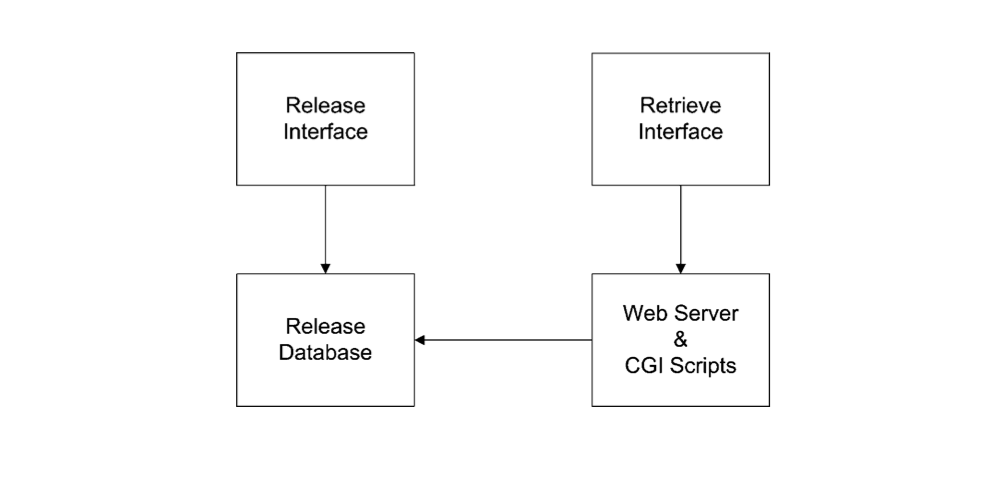
\includegraphics[width=\linewidth]{/Users/kenzie/Documents/HoGent/Bachelorproef/Images/SRM_Concept.png}
    \caption{Figuur uit \autocite{Hoek2002}. Figuur toont een simpele chart van hoe een software release management systeem opgebouwd kan zijn.}
    \label{fig:SRM_arch}
\end{figure}
De figuur~\ref{fig:SRM_arch} illustreert de architectuur van de software release management tool. Deze bestaat uit vier delen. Een logisch gecentraliseerde, maar fysiek gedistribueerde releasedatabase, een interface waarmee ontwikkelaars componenten in de releasedatabase plaatsen, een interface waarmee gebruikers componenten uit de releasedatabase halen en een webserver voor het op afstand toegang krijgen tot de releasedatabase en de componenten.
\newline
\newline
Deze paper \autocite{Hoek2002} stelt dus dat software release management ervoor moet zorgen dat componenten die op verschillende locaties, door verschillende bedrijven ontwikkeld worden, gemakkelijk gecentraliseerd toegankelijk moeten zijn. De bedrijven zelf hebben nog altijd volledige controle in handen van het versie beheer en het groeperen van de verschillende extern benodigde componenten. Tevens is de eindgebruiker nog altijd verantwoordelijk voor de installatie ervan maar dit begint ook minder het geval te zijn aangezien er meer en meer uitrol tools op de markt komen.
\newline
\newline
\subsection{Challenges and Problems in Release Management Process: A Case Study}
Zoals eerder aangehaald spelen ITIL-achtige procedures een belangrijke rol in software release management. Deze paper \autocite{Lahtela2011} is een korte casestudie met de bedoeling om kort een aantal problemen aan het licht te stellen in verband met software release binnen een bedrijf of organisatie naar een klant toe en hiervoor een oplossing aan te bieden.
\newline
\newline
De casestudie \autocite{Lahtela2011} beschrijft allereerst een definitie voor release management. “Release management omvat mensen, functies, systemen en activiteiten om software- en hardware versies effectief te plannen, verpakken, bouwen, testen en implementeren in een productie omgeving.”~\textcite{Lahtela2011} Deze definitie sluit goed aan bij wat we in dit onderzoek trachten te verduidelijken. Ook stelt de studie een redelijk belangrijk algemeen probleem. Helaas is in de praktijk bij veel bedrijven nog geen sprake van een implementatie van ITIL, ISO, enz. procedures. Dit omdat dit zeer moeilijk te implementeren is in reeds bestaande processen. Het hebben van zo een procedures is niet alleen zeer belangrijk om kwalitatief goede software op te leveren maar ook voor de supportafdeling van een bedrijf. Meestal zijn dit de mensen die het meeste te maken krijgen met deze procedures. Hierbij moet wel gezorgd worden dat er duidelijk verschil gemaakt wordt tussen het managen van veranderingen en het release management. Vervolgens beschrijft de studie de vastgestelde problemen en een mogelijk oplossing ervoor. Deze zijn letterlijk overgenomen uit de studie~\textcite{Lahtela2011}.
\begin{itemize}
    \item Er is geen gespecificeerd releasebeheerproces.
    \begin{itemize}
        \item Het releasebeheerproces moet worden beschreven en gestroomlijnd om ervoor te zorgen dat iedereen in de organisatie het proces kent.
    \end{itemize}
    \item De rol van releasemanager is onduidelijk.
    \begin{itemize}
        \item Iemand moet worden genoemd voor de rol van releasemanager. Daarnaast moeten de rollen, toewijzingen en verantwoordelijkheden worden beschreven.
    \end{itemize}
    \item De klant weet niet wat de release bevat.
    \begin{itemize}
        \item Meestal worden niet alle aangebrachte veranderingen beschreven of worden deze te technische beschreven waardoor de klant deze niet verstaat. De boodschap is om deze goed te documenteren op een verstaanbare manier.
    \end{itemize}
     \item De uitgifte distributie snelheid is te hoog.
    \begin{itemize}
        \item De release-vensters, die het tijdstip bepalen waarop de release in de productieomgeving van de klant moet worden geïnstalleerd, moeten worden overeengekomen tussen de serviceprovider en de klant, bijvoorbeeld grote releases maandelijks en kleinere releases wekelijks.
    \end{itemize}
    \item De klant denkt dat de serviceprovider niet alle testgevallen kan testen of inspecteren.
    \begin{itemize}
        \item Het testproces, dat deels wordt gedaan binnen het release managementproces, moet worden ontwikkeld. Het proces moet worden beschreven en aan producttesters worden geleerd. Daarnaast moeten de testresultaten aan de klant worden voorgelegd.
    \end{itemize}
    \item Er moeten meer testomgevingen in het testproces zijn.
    \begin{itemize}
        \item Er moet worden onderzocht of er meer testomgevingen nodig zijn. De ideale situatie is dat er voor elke productieomgeving een identieke testomgeving zou zijn.
    \end{itemize}
    \item Het verandermanagement van testomgevingen is onvoldoende.
    \begin{itemize}
        \item Elke wijziging die in een bepaalde testomgeving wordt aangebracht, moet correct worden gedocumenteerd. Op deze manier zijn alle wijzigingen traceerbaar en up-to-date.
    \end{itemize}
    \item Problemen bij versiebeheer.
    \begin{itemize}
        \item Alle versies van verschillende producten moeten worden gedocumenteerd in een klant specifieke lijst, die de serviceprovider vertelt welke geïnstalleerde productieversies de klant heeft.
    \end{itemize}
    \item De caseorganisatie heeft geen specifieke 'release jury'.
    \begin{itemize}
        \item Er is behoefte aan een specifieke jury die releases inspecteert voordat ze in productie worden genomen.
    \end{itemize}
\end{itemize}
Deze studie \autocite{Lahtela2011} biedt een unieke inkijk op een specifiek geval en biedt oplossingen aan voor bepaalde problemen. Sommige van deze problemen sluiten zeer goed aan bij dit onderzoek. Zo is er nood aan een zeer goede test omgeving zodanig dat er niet nodeloos over en weer moet gereden worden tussen klant en bedrijf. Dit onderzoek zal dan ook deze problematieken in acht nemen en proberen op te lossen in deze use case.

\subsection{Methodes and Systems for Software Release Management}
Het volgende document \autocite{Barshefsky2005} is een patent dat een bepaalde problematiek met normale software release management probeert te verhelpen. Op zich is dit patent niet zo interessant voor dit onderzoek maar de figuren en ideeën waarvoor het bedrijf in kwestie een patent heeft aangevraagd, kunnen wel helpen in het beter begrijpen van software release management en hoe deze wordt toegepast.
\newline
\newline
Dit document \autocite{Barshefsky2005} begint met zeer algemeen uit te leggen hoe software release management werkt en wat de verschillende stappen zijn die doorlopen worden. Het begint met versie beheer van de software. Waarna deze in een ontwikkelomgeving wordt gebracht. Hierna zal de software meestal naar een test omgeving gaan vooraleer het in productie wordt geplaatst. Al deze verschillende stappen zijn meestal verschillende mensen, in verschillende grote teams, die niets anders dat hun specifieke stap uitvoeren. Zie flowchart~\ref{fig:FL_fig1}.
\begin{figure}[H]
    \centering
    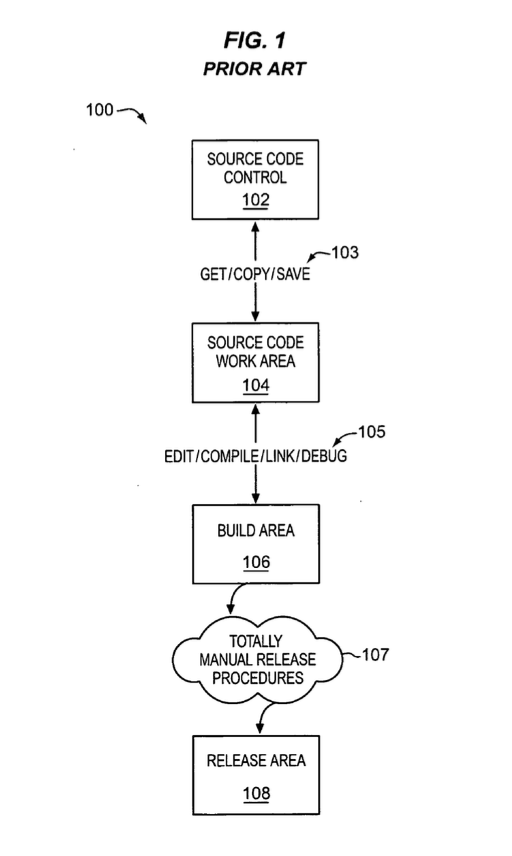
\includegraphics{/Users/kenzie/Documents/HoGent/Bachelorproef/Images/SRM_P_Fig1.png}
    \caption{Figuur uit \autocite{Barshefsky2005}. Flowchart van een niet geautomatiseerde versie beheer procedure.}
    \label{fig:FL_fig1}
\end{figure}
Het document \autocite{Barshefsky2005} beschrijft echter een aantal problematieken bij het idee uit figuur 1. Zo is dit een zeer manueel proces waarbij verschillende mensen deelnemen. Het is dus zeer gemakkelijk om fouten te maken tijdens een van deze stappen. Bijvoorbeeld een merge conflict. Deze hebben ze proberen te verhelpen door middel van computer geassisteerde release. Zie figuur 2. Ook is er in dit document nagedacht over de verschillende files en methodes om software te compileren en hoe deze beheerd moeten worden. Zo stellen ze gescheiden opslagplaatsen voor, voor inventory files en build files, enz. Zie figuur 3 voor details.
\newline
\newline
Dit document \autocite{Barshefsky2005} toont dus een nogal algemeen beeld over de software release cycli en wordt meer ter info beschouwd in dit onderzoek.
\newline
\newline
\subsection{Continuous Integration and Its Tools}
Bij release management hoort continuous integration en continuous development. Het volgende korte artikel \autocite{Meyer2014} bespreekt kort waarom een organisatie aan continuous integration moet doen en wat voor tools er allemaal bestaan. Ook worden er een aantal aanwijzingen gegeven rond het gebruik van continuous integration.
\newline
\newline
Het artikel \autocite{Meyer2014} vertrekt vanuit het stand punt dat een versie beheer tool in ieder softwarebedrijf een gegeven moet zijn. Dit om situaties te vermijden dat het lokaal werkt maar op andere toestellen niet. Ook staat dit toe om volledige geautomatiseerde pipelines te maken die automatisch de code gaat compileren en controleren op fouten door meegeleverde testen of door een uitrol te doen, in een test omgeving. Het artikel gaat verder met te stellen dat het bij iedere organisatie een prioriteit moet zijn om ten aller tijden de builds werkende te houden. Dit staat dan niet alleen toe dat er ten allertijden een uitrol kan gedaan worden van werkende code naar een test omgeving, maar ook dat er geen fouten of niet werkende code wordt gepusht door de ontwikkelaars. Het artikel beschrijft verder een aantal tools zoals onder andere Jenkins voor het automatisch uitrollen en testen van nieuwe software.
\newline
\newline
Dit artikel \autocite{Meyer2014} is minder belangrijk voor dit onderzoek maar toont wel het belang aan van een build pipeline en een goeie test omgeving voor code werkende te houden en de kwaliteit de behouden.
\newline
\newline
\subsection{DeVops}
Devops is de overkoepelende term van release management en continuous integration and continuous development. Het is de bedoeling om de verschillende softwareteams onderling te doen communiceren en samenwerken. Dit met doel om beter en sneller software uit te rollen. Het volgende artikel \autocite{Ebert2016} legt in meer detail Devops uit. De 2 luiken van Devops worden besproken alsook waarom Devops belangrijk is. Ook worden veel tools en technieken aangehaald.
\newline
\newline
Het artikel \autocite{Ebert2016} begint met uit te leggen wat Devops voor een organisatie kan betekenen. Het stelt dat Devops staat voor een betere samenwerking tussen ontwikkelen, kwaliteit, zekerheid en operaties. Het is lang niet zo dat Devops voor ieder softwareproject kan gebruikt worden, maar het wordt toch aangeraden. Ook vertrekt het artikel uit een gegeven dat er al softwareversie beheer in enige vorm aanwezig is.
\newline
\newline
Verder stelt het artikel \autocite{Ebert2016} dat er 2 facetten zijn bij Devops. Enerzijds de build kant van de software en anderzijds het deployment gedeelte van de software. Builden wordt volgens het artikel hoofdzakelijk op twee manieren gedaan. Aan de ene kant zijn er de traditionele build tools die meestal nog wat handmatig werk vereisen. Om in deze tools een build te doen moet er meestal een xml gemaakt worden met specifieke onderdelen. Dit kan nogal arbeidsintensief zijn. Langs de andere kant zijn er contiuous integration procedures. Hierbij wordt getracht om op ieder moment test bare werkende code te hebben. Deze tools zijn een stuk gemakkelijker om te gebruiken en zijn meestal cloud gebaseerd. Dit is omdat het de bedoeling is om op een zeer vlot en sneller tempo updates te kunnen uitrollen. Het artikel beschrijft een tabel~\textcite{Ebert2016} waarin een aantal tools met wat rand info beschreven staan.
\newline
\newline
Het artikel \autocite{Ebert2016} stelt dat meestal hierna de software getest moet worden zodanig dat kwaliteit kan worden gegarandeerd. Dit moet zo efficiënt en snel mogelijk gebeuren waardoor er dus nood is aan infrastructure as code. Herbruikbare code die snel kan worden uitgevoerd over meerdere platformen. Verschillende automatisatie tools worden door het artikel besproken. De meeste zijn simpel in gebruik en gebruiken yaml of xml voor de test omgevingen te definiëren. Het uitrollen van test omgevingen voor de software wordt meestal in de cloud gedaan of met virtuele machines. Dit is afhankelijk van wat de vereisten zijn van de organisatie. 
\newline
\newline
Ook bespreekt het artikel \autocite{Ebert2016} een van de nieuwere manieren om software te testen. Ze bespreken het gebruik van microservices in de cloud. Hoofdzakelijk bespreekt het artikel de producten van Amazon AWS. Deze zijn zeer gemakkelijk te automatiseren en gemakkelijk in gebruik.
\newline
\newline
Dit artikel \autocite{Ebert2016} is een meer waarde voor dit onderzoek omdat er een hele hoop tools, naast elkaar, kort besproken worden. De nadruk ligt niet op gebruiksvriendelijkheid maar eerder op wat de tools ondersteunen en of dat ze snel bruikbaar zijn voor Devops procedures. Dit artikel bevestigd dat er in de use case van dit onderzoek een nood is aan een goed gebouwde omgeving omdat kwaliteit een nummer een prioriteit geworden is.
\newline
\newline
\section{Amazon AWS}
\subsection{Performance Analysis of High Performance Computing Applications on the Amazon Web Services Cloud}
Dit onderzoek wil ook de cloud platformen en hun aanbod naast elkaar leggen. Ook wilt dit onderzoek vlug een idee krijgen hoe de verschillende datacenters van de cloud providers samengesteld zijn en hoe de verbindingen hiermee zijn. De volgende paper \autocite{Jackson2010}is een prestatie test van een Amazon aws datacenter.
\newline
\newline
De paper \autocite{Jackson2010} gebruikt synthetische wetenschappelijke testen om de prestatie van een aantal Amazon producten te testen. Een Amazon datacenter is wat raar samengesteld aangezien de eindgebruiker geen enkel idee op voorhand heeft over welke hardware hij toegewezen krijgt in het datacenter. Bovendien is Amazon benadeelt op vlak van connectiviteit omdat het niet directe lijnen heeft naar de datacenters zoals Microsoft met Azure. Belangrijk is dat alle testen uitgevoerd door de paper, uitgevoerd zijn in hetzelfde datacenter.
\newline
\newline
In deze paper \autocite{Jackson2010} testen de onderzoekers vooral of dat een Amazon datacenter geschikt zou zijn voor wetenschappelijk gebruik. Vandaar dat er vooral synthetische wetenschappelijke tools gebruikt worden. De tools zijn zorgvuldig geselecteerd zodanig dat de verschillende aspecten van een datacenter worden getest. Zowel de processor, als RAM, de harde schijven en ook de verbinding met de servers worden getest.
\newline
\newline
De paper \autocite{Jackson2010} concludeert dat de prestatie van de systemen wel goed is maar dat het afhankelijk is van welk merk CPU de gebruiker krijgt. Aangezien hier geen controle over is, is het moeilijk om voor dezen redenen Amazon voor rekenintensieve doeleinden aan te raden. Ook is vastgesteld dat de connectie met het datacenter een aanzienlijke limitatie is voor taken die zeer transactie intensief zijn.
\newline
\newline
Deze paper \autocite{Jackson2010} is niet zo zeer een meerwaarde voor dit onderzoek. Het artikel is redelijk verouderd en ondertussen is Amazon een van de grotere cloud platformen. Ook bespreekt deze paper niet zo goed de producten van Amazon. Ook is de use case die de paper beschrijft totaal verschillend van de use case die dit onderzoek gebruikt. 
\newline
\newline
\section{Microsoft Azure}
\subsection{Microsoft Azure and cloud computing}
Aangezien binnen de use case van dit onderzoek Microsoft Azure een grote rol speelt, is het belangrijk om een zeer goed idee te vromen van hoe die cloud platform in elkaar zit en wat de verschillende services en producten zijn. Daarom is het volgende hoofdstuk uit een boek \autocite{Copeland2015} redelijk informatief, zeker om ergens te starten.
\newline
\newline
Het eerste hoofdstuk uit het boek \autocite{Copeland2015} is vooral bedoelt als een eerste kennismaking met het Azure platform. Azure is eigenlijk ontstaan uit Microsoft hun office 365 aanbiedingen. Microsoft biedt een grote hoeveelheid aan applicaties aan als onder deel van dit pakket. Omdat die applicaties ergens moeten draaien, is Microsoft begonnen met het bouwen van datacenters om daar hun SaaS (Software as a Service) in te hosten. Al snel beseften ze dat er geld viel te verdienen met het aanbieden van remote services. Het duurde dan ook niet lang vooraleer Microsoft ook begon met IaaS (Infrastructure as a Service) aan te bieden. Dit was toen een unicum volgens het boek \autocite{Copeland2015}, Aangezien tot dan de meeste cloud platformen ontstaan zijn vanuit het verhuren van overschot aan computing power uit een mengelmoes van toestellen uit een bepaald datacenter. Dit was onder andere een van de conclusies van een verouderd artikel over Amazon aws \autocite{Jackson2010}. Bij Microsoft waren dat speciaal gebouwde datacenters met die services in gedachten. Ook hun PaaS (Platform as a service) wordt kort aangehaald door het boek \autocite{Copeland2015}.

\textbf{Voorbeelden van Azure Iaas:}
\begin{itemize}
    \item Azure virtual machines
    \item Azure virtual networks
    \item Azure virtual networks gateways
    \item Azure storage solutions
    \item ...
\end{itemize}
\textbf{Voorbeelden van Azure Paas:}
\begin{itemize}
    \item Azure SQL database
    \item Azure website
    \item Azure content delivery network
    \item Azure DeVops
    \item ...
\end{itemize}
Verder legt het boek  \autocite{Copeland2015} kort uit wat vanuit Azure gedaan wordt op vlak van privacy en wetgevingen. Dit is minder interessant voor dit onderzoek. Ook gaat het boek kort in op waarom gebruikers, It professionals voor Azure cloud of een ander cloud platform zouden moeten kiezen. Zo haalt het boek  \autocite{Copeland2015} aan dat een cloud platform weinig onderhoud inhoud, minder dan een lokale opstelling. Ook is de eindgebruiker niet verantwoordelijk voor de hardware. Hun datacenter zijn redundant. Dus er is eigenlijk vrij weinig downtime. Ook de aangeboden producten zijn vrij compleet en gemakkelijk onderhoudbaar.
\newline
\newline
Verder geeft het boek  \autocite{Copeland2015} een korte introductie in het Azure web portaal. Deze heeft dit onderzoek voor kennismaking doeleinden eens doorgelopen. Veel interessants is hier voor dit onderzoek niet uit te melden. Het hoofdstuk is dus een snelle kennismaking met Azure. Dit dient als een basis voor verder onderzoek. Zo gaan we in deze literatuurstudie nog wat dieper in op Azure DeVops en een kleine hands-on. Ook IaaS van Azure wordt nog wat meer uitgediept.
\newline
\newline
\subsection{Microsoft Azure Documentation}
Zoals eerder aangehaald in deze literatuurstudie, speelt Microsoft Azure een belangrijke rol binnen de use case van dit onderzoek. Het is het vertrek punt voor de vergelijkingen. In het kader van dit onderzoek, is de website van Azure eens uitgeplozen. Dit omdat er een beeld kan gevormd worden over welke Azure services interessant kunnen zijn. Het volgende is een kort verslag. Er worden twee service categorieën aangehaald. Deze zijn Iaas en PaaS (Infrastructure as a Services en Platform as a Service). Specifiek is er gekeken naar Azure virtual machine, Azure virtual networks, Azure virtual gateways en Azure DeVops. Het laatste is een samenvatting van een onlinecursus van een uur en informatie op Microsoft Docs.
\newline
\newline
In het kader van software release management en dan vooral de stap om de kwaliteit van software te controleren, is er gekeken of er misschien een mogelijkheid is om deze specifieke infrastructuur eventueel in de cloud te maken. Hiervoor is er een kort concept uitgewerkt. Dit concept beschrijft een hybride infrastructuur (verwijzing) waarbij eigenlijk alle niet use case specifieke toestellen in de cloud zitten. In theorie stond dit toe dat alle infrastructuur dan als code zou kunnen worden gedefinieerd.
\newline
\newline
Het aanbod qua mogelijkheden voor hardware om een virtuele machine aan te maken op Azure is enorm. Ook in tegenstelling tot de concurrenten wordt er zeer transparant omgesprongen met welke hardware er per optie beschikbaar gesteld wordt. De mogelijkhden verschillen enorm en zijn meestal voor specifieke doeleindes. Ook de prijzen schalen mede met de use cases. Zo zijn er specifieke opties voor machine learning. Of een optie voor machines met enorme hoeveelheden ram en CPU-kracht om met bepaalde databases overweg te kunnen. Ook de goedkopere basis opties zijn redelijk uitgebreid. Al deze opties worden door Azure onderverdeelt in categorieën die door middel van een letter worden aangeduid. Zie figuur~\ref{fig:Chart_Azure_tiers}.
\begin{figure}[H]
    \centering
    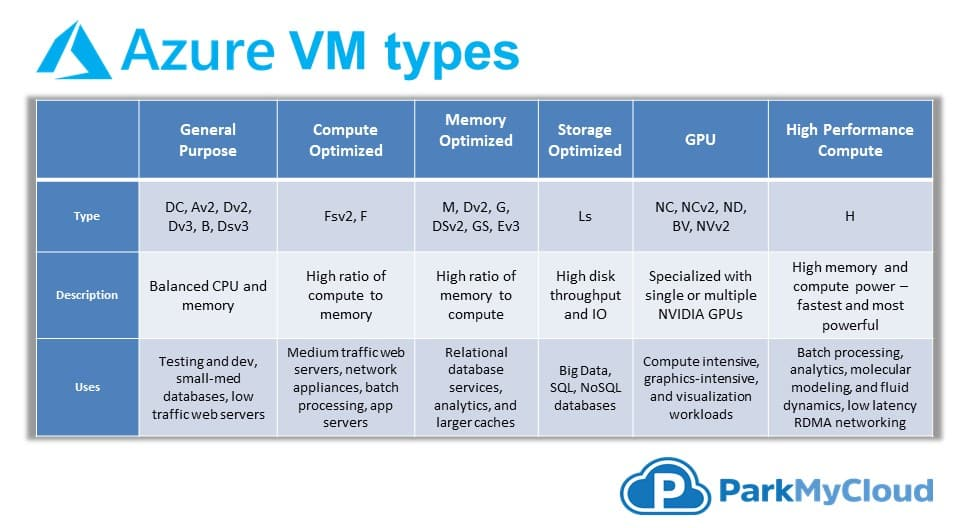
\includegraphics[width=\linewidth]{/Users/kenzie/Documents/HoGent/Bachelorproef/Images/azure-vm-types-comparison-1.jpg}
    \caption{Figuur van (https://p2zk82o7hr3yb6ge7gzxx4ki-wpengine.netdna-ssl.com/wp-content/uploads/azure-vm-types-comparison-1.jpg). Chart met alle VM tiers van azure en hun specifieke code.}
    \label{fig:Chart_Azure_tiers}
\end{figure}
Verder is Azure de oudere manier van het definiëren van een Azure virtual machine aan het afraden. Hiernaast zijn er ook nog een tal van mogelijkheden op vlak van virtual networking. Het belangrijkste is dat er een mogelijkheid bestaat om een virtueel netwerk volledig te isoleren van het internet. Dit staat toe dat enkel verkeer dat op dat specifieke netwerk is, aan de virtuele machines kan. Er wordt dan wel meestal een Azure network firewall node voorzien die in dit virtueel netwerk zit, zodanig dat de connectiviteit met de machines ten aller tijden gegarandeerd kan worden. Om dan connectiviteit te hebben met het virtueel netwerk wordt er gebruikgemaakt van een Azure Gateway node. Deze staat een point to point VPN (Virtual Private Network) tunnel toe. Dit is eigenlijk een directe, encrypteerde verbinding met het Azure netwerk. Hiervoor is wel specifieke hardware nodig lokaal in het netwerk. De kost van deze services is eigenlijk bijna niks. Azure werkt immers met een pay-to-run, pay-on-the-go system. Dit wil zeggen dat er dus moet betaald worden voor de aanmaak van de services en daarna voor het verbruik. Microsoft heeft op zijn documentatie portaal tal van stap voor stap handleiding voor het instellen van deze services. Ook concepten voor hybride opstellingen staan hier uitgelegd. Maar dit zou deze literatuurstudie te veel doen afwijken.
\newline
\newline
Het zou dus in theorie mogelijk moeten zijn om een hybride cloud infrastructuur te voorzien die dynamisch is voor de specifieke te testen projecten. De vraag is of dit handig is in gebruik en niet nodeloos complexiteit toevoegt.
\newline
\newline
Aure Devops in een platform van Azure dat organisaties toestaat om bepaalde procedures te definiëren voor het uitrollen van projecten. Het platform staat dan ook integratie toe met andere project follow-up tools van Microsoft. Deze procedures kunnen juist zoals de virtuele machines op Azure via code worden gedefinieerd of via een duidelijk en gemakkelijk te gebruiken GUI. De bedoeling van Azure DeVops is eigenlijk om het oude TFS-systeem te vervangen en een verbeterde interface aan te bieden. Meestal wordt DeVops gebruikt om aan Continuous Integration te doen. Dus er wordt een repository waar de code opstaat gedefinieerd. Hierna bestaat er een mogelijkheid om de code te compileren, automatisch testen te runnen en deze code dan weer door te schuiven naar een volgend stadium. Hier wordt de code dan uitgerold naar een omgeving voor verder kwaliteitscontrole. Het mooie aan dit platform is dat de gebruiker of organisatie niet verplicht is om deze code in een virtuele machine in de cloud te compileren of testen. Er is volledige controle over de procedures.
\newline
\newline
In het kader van dit onderzoek is dit zeer belangrijk aangezien dit platform op dit moment in gebruik genomen wordt. Er is ook een onlinecursus gevolgd met een basis uitleg en een labo. Dit heeft duidelijk gemaakt dat het mogelijk is om vanuit DeVops op een lokale test omgeving uit te rollen.
\newline
\newline
%%=============================================================================
%% Methodologie
%%=============================================================================

\chapter{\IfLanguageName{dutch}{Methodologie}{Methodology}}
\label{ch:methodologie}

%% TODO: Hoe ben je te werk gegaan? Verdeel je onderzoek in grote fasen, en
%% licht in elke fase toe welke stappen je gevolgd hebt. Verantwoord waarom je
%% op deze manier te werk gegaan bent. Je moet kunnen aantonen dat je de best
%% mogelijke manier toegepast hebt om een antwoord te vinden op de
%% onderzoeksvraag.
Aucxis werkt momenteel hoofdzakelijk met ‘.NET’ projecten. Als IDE wordt er Visual Studio gebruikt. Als versiebeheer gebruiken ze hiervoor TFVC. Dit was een voor een lange tijd een goede oplossing. De testen die werden uitgevoerd waren vooral functionele testen. Dit is niet ideaal. Er wordt op moment van implementatie bij klanten veel fouten en bugs vastgesteld waardoor er enerzijds veel frustratie ontstaat bij de mensen die het uitrollen bij een klant. Anderzijds wordt er veel tijd en geld verloren met het over en weer verplaatsen tussen klant en bedrijf. Aucxis heeft recent een keuze gemaakt om meer te investeren in kwaliteit. Aangezien Aucxis al een verwent gebruiker van Microsoft is, was de keuze voor Azure DeVops niet moeilijk. Ook heeft dit minder impact op hun huidige werkwijze.

Zoals eerder aangehaald worden er vooral functionele testen uitgevoerd. Met de stap naar kwalitatievere oplossingen is er ook nood voor meerdere soorten testen. Het ideale zou zijn dat er naast functionele testen ook in een gecontroleerde omgeving, die een situatie bij de klant in kwestie nabootst, getest kan worden. Daarna zou het programma bij een test omgeving van de klant uitgerold worden om daar te worden getest. In een finale stap, zou het programma dan in productie worden uitgerold. Dit alles zou zo geautomatiseerd mogelijk moeten verlopen.

Azure DeVops lijkt hier het meest geschikt voor om deze functionaliteit te verkrijgen. Daarom de vraag om toch het aanbod van Azure met de andere Cloud platform aanbieders te vergelijken en het beste alternatief te selecteren. Om dit te bereiken is er in dit onderzoek begonnen met kort de verschillende Cloud platformen hun aanbod naast elkaar te leggen.

\section{Vergelijking}
\subsection{Azure DeVops}
Microsoft Azure is gelanceerd in 2010 en bevat een hele serie producten. Azure biedt vooral producten aan in de categorieën Software as a Service (SaaS), Infrastructure as a Service (Iaas) \& Platform as a Service (PaaS). Azure heeft een aantal zeer goede producten voor virtualisatie. Zo Biedt Azure een enorm aanbod aan verschillende soorten machines aan voor verschillende doeleindes. Ook hun virtuele netwerkmogelijkheden zijn enorm. Dit alles is mooi geordend en zeer gemakkelijk in gebruik. De Azure datacenters zijn over heel de wereld verspreid. Deze zijn altijd het nieuwste van het nieuwste en zijn zeer goed verbonden onderling en met de buitenwereld. Omdat Azure van Microsoft is, is Azure ook perfect te integreren met bestaan gebruikers accounts in domeinen. Dit geeft de gebruiker volledige controle over wie wat kan gebruiken en zien. Azure biedt ook een aantal services aan. Daarvan is Cloud gebaseerde Active Directory er een van. Ook bieden ze een volledig aanbod aan services aan om een CI/CD pijpleiding te realiseren.

Azure DeVops was vroeger bekend als Visual Studio Team System (VSTS) of Team Foundation Server (TFS). Het is een versie beheer, rapportering, vereisten beheer, project beheer, automatisch compileer, test en uitrol beheer tool gemaakt door Microsoft. De tool maakt gebruik van Team Foundation Version Control (TFVC) of Git. De tool is gemaakt om de volledige levenscyclus van een programma te controleren en beheren. Ook biedt de tool de mogelijkheid aan programmeerteams om in een DeVops sfeer samen te werken. Het mooie aan deze tool is dat het bijna in iedere Integrated Development Environment (IDE) te integreren is.

Het is mogelijk om deze tool zowel lokaal als in de Cloud te implementeren. Microsoft heeft deze tool toegevoegd aan hun Azure aanbod onder Azure DeVops. Microsoft heeft de verschillende componenten van deze tool opgesplitst op het platform. Dit maakt het mogelijk dat de gebruiker niet alle componenten tegelijk hoeft te gebruiken of te implementeren. De gebruiker kan zo naar hun voorkeur functie kiezen.

Azure DeVops kan gebruikmaken van twee soorten versie controle in een project. Het kan gebruikmaken van de door Microsoft speciaal ontwikkelde versie beheer framework TFVC voor Azure DeVops of het wereld befaamde Git. 

TFVC ondersteund twee manieren van werken, met een centraal systeem of lokaal met check-out/ check-in op de computer van de programmeur. Bij het gebruik van een centraal systeem worden files die door een andere programmeur gebruikt worden als ‘alleen lezen’ bestempeld. Dit kan leiden tot problemen als andere programmeurs deze files nodig hebben voor bepaalde zaken. Dit heeft Microsoft proberen oplossen door het mogelijk te maken om volledig lokaal te werken. De programmeur kan dan alle files aanpassen waar nodig. Eventuele problemen met verschillende files moeten dan worden opgelost bij check-in. Dit maakt het mogelijk dat er veel minder conflicten ontstaan. Een ander voordeel is dat de gebruiker de mogelijkheid heeft om met TFVC, regels te configureren die bij check-in worden uitgevoerd.

Git is een veel gebruikt versie beheersysteem. Bijna alle IDE’s bieden ondersteuning aan voor dit systeem. Het werkt gelijkaardig zoals TFVC. Alleen kan de gebruiker met Git geen regels configureren die worden uitgevoerd bij check-in. Git is wel volledig compatibel met Azure DeVops. Zo kan er rechtstreeks met Git op Azure DeVops gepubliceerd worden. Dit alles zorgt ervoor dat gebruikers door gebruik van Git, met bijna iedere IDE of programmeertaal, Azure Devops kan gebruiken. 

Een ander voordeel van Azure DeVops is de uitgebreide rapportering ingebouwd in de tool. Deze maakt het mogelijk om uitgebreide verslagen te genereren van de uitgevoerde testen, een uitgevoerde check-in, compilatie problemen, enz. Ook staat het de gebruiker toe om gepaste meldingen te versturen of automatisatie te configureren om bepaalde problemen op te lossen. Daarnaast heeft Azure Devops ook een ingebouwde tool om planningen voor projecten bij te houden.

Azure Boards is letterlijk een volledige implementatie rechtstreeks in Azure DeVops van een scrum bord. Zo kan de gebruiker bij het opleveren van een uitgevoerde taak automatisch de compilatie pijpleiding laten starten. Ook is het volledig geïntegreerd met GitHub waardoor de gebruiker geen extra kosten moet maken om een Azure Repository aan te maken. Ook bestaat de mogelijkheid om Azure boards naadloos te laten samenwerken met de populairste chat applicaties voor ontwikkelaars, zoals Slack.

In Azure DeVops als een gebruiker een CI pijpleiding wil configureren, kan de gebruiker dat simpel via de web interface doen of met de Azure powershell add-on. Azure DeVops gebruikt zoals eerder vermeld, twee soorten versie beheer tools. Om met Git een pijpleiding te bouwen selecteert de gebruikt simpel weg als bron een git repository. Daarna kan de gebruiker kiezen uit een hele serie voor gemaakte motoren voor het compileren van de code. Ook door gebruik te maken van een marktplaats kunnen er zelfs volledig aangepaste motoren gebruikt worden. Hierna wordt de gebruiker gevraagd om een azure-pipelines.yml aan te maken in de broncode waarin dan de configuratie geschreven wordt voor de uit te voeren compilatie. De gebruiker kan dan nog stappen toevoegen voor testen uit te voeren. Azure DeVops heeft de mogelijkheid om op verschillende manieren de software uit te rollen. Gaande van in de Cloud naar specifieke lokale omgevingen enz.

Azure Devops prijzen worden beschreven in figuur~\ref{fig:A_DO_Money}.

\begin{figure}[!htbp]
    \centering
    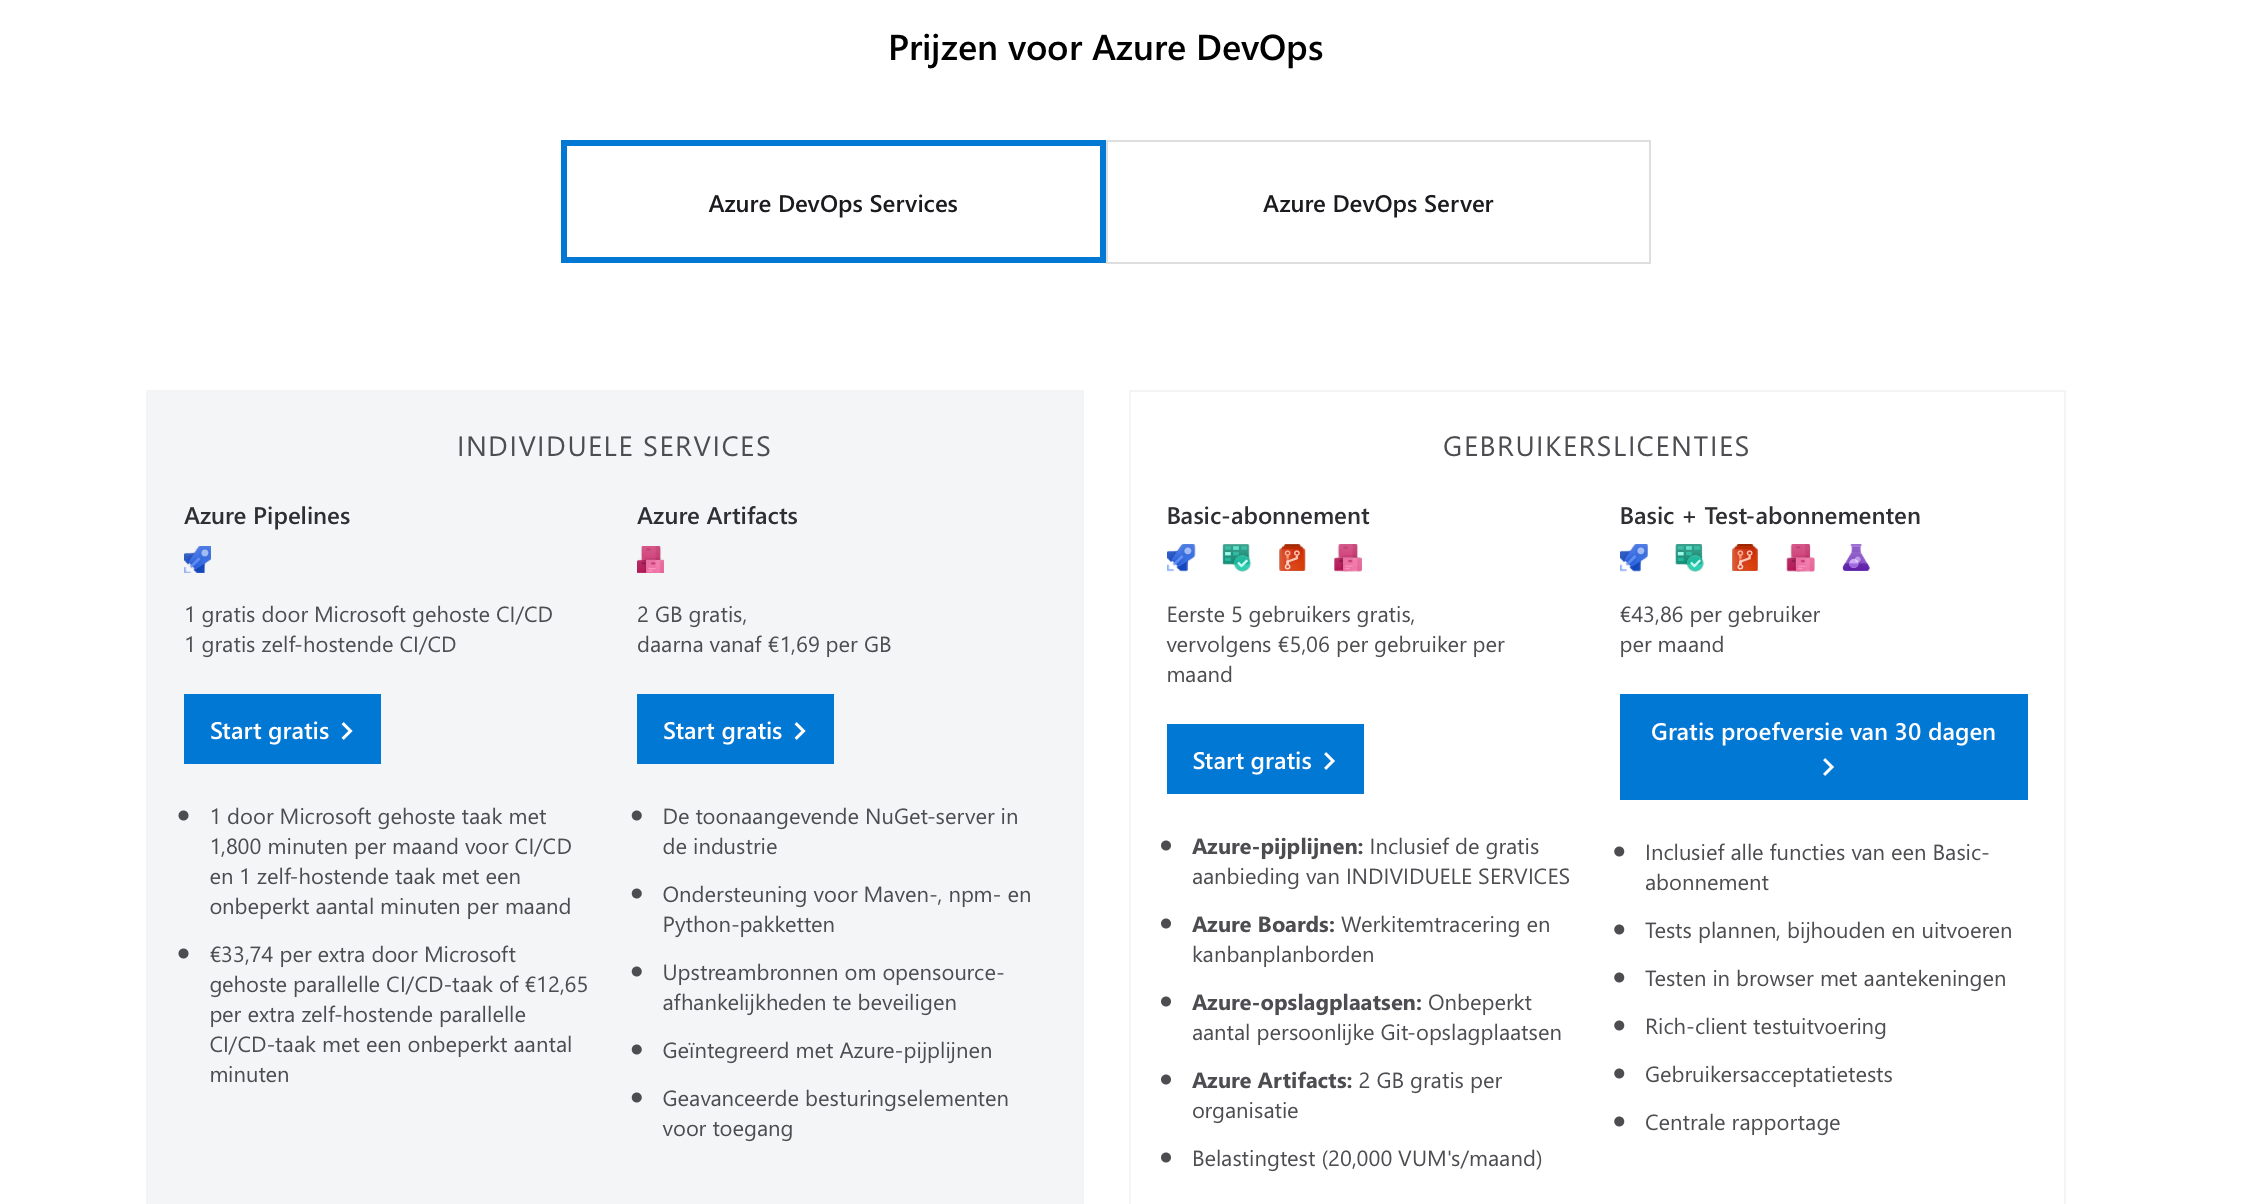
\includegraphics[width=\linewidth]{/Users/kenzie/Documents/HoGent/Bachelorproef/Images/Azure_DO_money.png}
    \caption{Figuur van \href{https://azure.microsoft.com/nl-nl/pricing/details/devops/azure-devops-services/}{Azure DeVops website}. Figuur toont de prijzen voor Azure DeVops op een beknopte manier.}
    \label{fig:A_DO_Money}
\end{figure}

Azure DeVops is in dit onderzoek het vertrekt punt voor de vergelijkingen. Dit omdat het perfect met de huidige werkwijze van Aucxis integreert en omdat zij reeds Microsoft partner zijn. In alle vergelijkingen zal gekeken worden of Git gebruikt kan worden omdat dit het een stuk gemakkelijker maakt voor de vergelijkingen. Aucxis ontwikkelt veel applicaties in .NET Core en daarom moet er ook gekeken worden of de alternatieve hiervoor compatible zijn. Azure DeVops is dus het zeer capabele vertrek punt voor de vergelijkingen met de andere Cloud platform aanbieders.
\subsection{Google Cloud}
Google Cloud Platform (GCP) is gelanceerd in April 2008. Het draaide des tijds in dezelfde datacenters als ‘google search’, ‘youtube’ en ‘gmail’. Het was slechts in 2011 dat GCP beschikbaar was voor het brede publiek. GCP is een onderdeel van de Google Cloud. Google Cloud biedt een enorme serie van producten aan waarvan GCP maar een klein onderdeel is. GCP specifiek, biedt ‘infrastructure as a service’ (IaaS), ‘platform as a service’ (PaaS) en ‘serverless computing’ aan. 

Omdat het doel van dit onderzoek specifiek de support voor CI/CD pijpleidingen vergelijken is, bekijken we een specifiek onderdeel van GCP. De ‘Cloud Developper Tools’. Onder deze categorie vallen er een aantal zeer interessante tools. Hier vindt men onder andere ‘Cloud Build’, ‘Cloud-SDK’, ‘Tools voor Powershell’, ‘Tools voor Visual Studio’, enz.

Cloud Build is Google zijn antwoord op een volledige geautomatiseerde CI/CD pijpleiding. Het is dan ook volledig mede met de moderne vereisten. Met Google Cloud Build (GCB) is een organisatie instaat om snel en gemakkelijk een volledige pijpleiding te configureren. Het gelijkt dan ook op Azure DeVops.

GCB werkt hoofdzakelijk met Git en GitHub om een pijpleiding te bouwen. Google heeft ook zijn eigen ‘Cloud repository service’ die naadloos integreert met GCB, maar deze is helaas betalend. Daarom is het gebruik van Git met GitHub een beter en goedkoper alternatief. Aangezien deze ook perfect integreren met GCB en omdat Git wijdverspreid en simpel in gebruik is. Een organisatie kan dan configureren op GCB dat bij het moment van een code update op GitHub, automatisch een compileer pijpleiding wordt gestart. Om GCB te laten weten wat er specifiek moet uitgevoerd worden, moet er op de GitHub repository een YML-file voorzien worden waarin regels gedefinieerd moeten worden. Dit maakt het gemakkelijk om snel aanpassingen te maken.

De pijpleiding op GCB werkt op basis van Docker images. Deze worden in de cloudbuild.yml gedefinieerd. Ook wordt er per Docker container gedefinieerd wat er moet uitgevoerd worden in de vorm van commando’s, script, enz. Dit maakt het mogelijk dat iedere stap in het CI gedeelte van de pijpleiding volledig aangepast kan worden naar de noden van de organisatie. Zo kan de organisatie beslissen om voor gemaakte containers te gebruiken van de ‘DockerHub’ pagina. Ook kan de organisatie zelf container maken met aangepaste scripts om bijvoorbeeld in lokale omgevingen testen uit te voeren. GCB kan dus in een hybride opstelling geïmplementeerd worden. Wat ook de bedoeling zou zijn aangezien dit een use case van Aucxis is. Daarnaast biedt GCB ook de mogelijkheid om de gecompileerde code rechtstreeks vanuit Google Cloud beschikbaar te maken voor verdere verdeling.

Met behulp van deze containers kunnen dan functionele testen uitgevoerd worden op de gecompileerde code. Het programma kan dan op basis van de uitkomst van deze uitgevoerde taak, naar de volgende stap zijn wachtrij worden geplaatst. Hier kan dan de volgende taak starten. GCB genereert rapporten en statistieken van de uitgevoerde taken zodanig dat de gebruiker van het platform inzicht kan krijgen in de uitgevoerde taken.

De compilatie en uitvoer-tijden van GCB zijn zeer goed aangezien het platform automatisch schaalt naarmate er meer rekwesten tegelijk verstuurd worden. Dit maakt mogelijk dat verschillende programmeurs tegelijk aan hetzelfde project werken of aan meerdere projecten tegelijk. Ook biedt GCB de mogelijkheid om redundantie te voorzien. GCB maakt het mogelijk om naar andere Cloudplatformen uit te rollen of zelfs om de werklast te verdelen over verschillende Cloud platformen. Dit is mogelijk door gebruik te maken van Tekton. Tekton is een open-source framework voor Kubernetes. Dit maakt het mogelijk dat een organisatie over verschillende Cloud platformen heen kan werken. Kubernetes is een clustering hypervisor voor Docker containers. Tekton zou een goede oplossing kunnen zijn voor CI/CD pijpleidingen in de Cloud maar valt hier buiten beschouwen vermits het doel de verschillende aanbiedingen van de Cloud platformen vergelijken is.

De prijzen in Google Cloud worden berekend zoals bij ieder moderne Cloud aanbieder. De gebruiker betaald wat hij verbruikt. De volgende figuur~\ref{fig:GCP_BC_money} moet dienen om een beeld te vormen over wat men kan verwachten te betalen voor het gebruik van GCB. Dit zonder netwerk kosten voor het transfereren van gegevens. Er wordt ook niks in rekening gebracht voor zaken die in een wachtrij staan of pijpleidingen die niet gebruikt worden. De Google Cloud Developper Tools hebben een voordeel dat een groot deel van de tools voor ondersteuning met het platform gratis zijn. Er zijn ook weinig tools van derden nodig om de gewilde functionaliteit te bereiken.

\begin{figure}[!htbp]
    \centering
    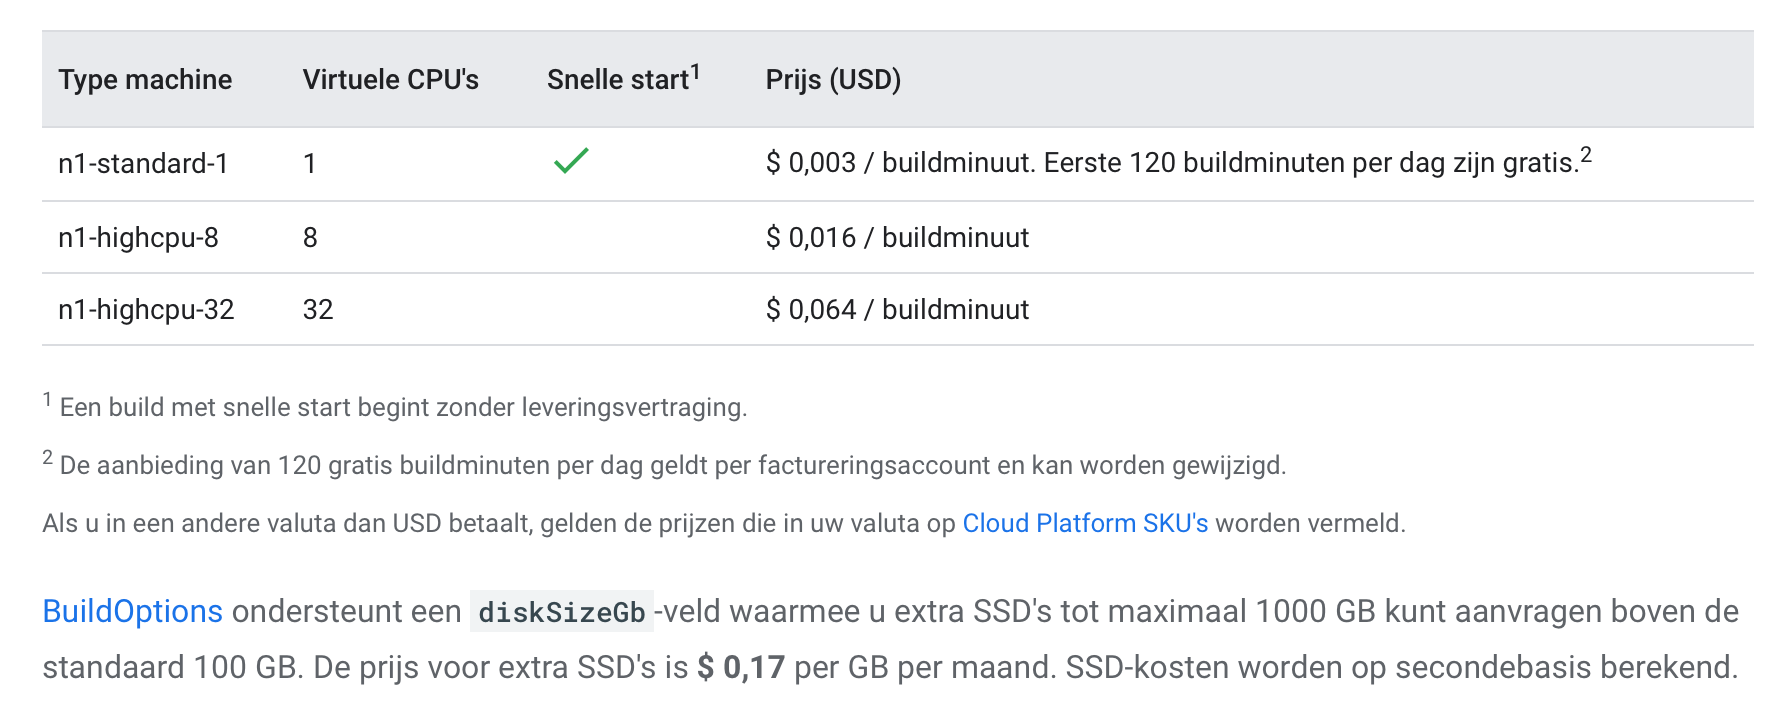
\includegraphics[width=\linewidth]{/Users/kenzie/Documents/HoGent/Bachelorproef/Images/gcp_bc_money.png}
    \caption{Figuur van \href{https://cloud.google.com/cloud-build/pricing}{Google Cloud website}. Figuur toont de prijzen voor Google Cloud Platform op een beknopte manier.}
    \label{fig:GCP_BC_money}
\end{figure}

Met andere woorden is GCB dus een volwaardig alternatief voor Azure DeVops. Er is ondersteuning voor verschillende tools, biedt uitgebreide functionaliteiten aan en bovendien adverteert Google dat het gemakkelijk samenwerkt met andere Cloudplatformen. Het zei door het gebruik van Tekton. Daarnaast is het ook relatief simpel in gebruik door dat GCB gebruikmaakt van Docker containers voor te compileren.

\subsection{Amazon Web Services}
Amazon web services (AWS) is gelanceerd in 2006. Gedurende lange tijd heeft Amazon stukken van hun datacenter verhuurd aan het brede publiek. Tegenwoordig kan een gebruiker op AWS een Cloud computer samenstellen juist zoals een gewone server samengesteld zou worden. Het is maar in recente tijden dat Amazon zich meer beginnen focussen is op services die de gebruiker kan gebruiken. Zo bevat AWS nu meer dan 212 services en producten. Bijvoorbeeld: virtuele computerkracht, netwerking, opslag in de Cloud, databases, statistieken, programma services, uitrol op de Cloud, beheer van bepaalde zaken, programmeertools en tools voor Internet Of Things (IoT). De populairste tegenwoordig zijn Amazon Elastic Compute Cloud (EC2) en Amazon Simple Storage Service (Amazon S3). Deze laatste zijn in feite Cloud computerkracht en opslag voor van alles die volledig schaalbaar zijn en die geen kosten hebben om aan te maken.

Ondanks dit groot aanbod resteert er toch nog altijd de vraag hoe het zit met de huidige prestatie van Amazon datacenters over de hele wereld. Zeker na het lezen van deze paper \autocite{Jackson2010}. Voor dit onderzoek is er ijverig gezocht naar recentere prestatie onderzoeken maar zonder resultaat. Er kan alleen maar afgegaan worden van Amazon zijn website.

Al deze producten en services maken het niet gemakkelijk voor een gebruiker om snel te weten welke producten juist voor hem geschikt zijn. Ook in dit onderzoek is er vastgesteld dat het lastig was om een duidelijk beeld te krijgen wat er allemaal aangeboden wordt. Dat terzijde, heeft Amazon toch een specifiek aanbod om CI/CD pijpleidingen te implementeren op hun Cloud platform. Zo heeft Amazon, AWS CodePipeline. Dit is een service waarbij de gebruiker of organisatie via het web portaal gemakkelijk een CI/CD pijpleiding kan definiëren. Deze is volledig aanpasbaar naar de noden van de gebruiker. AWS CodePipeline gebruikt AWS CodeBuild voor de compilatie en het testen van projecten in CI/CD en AWS CodeDeploy voor de automatische uitrol van projecten.

Zoals alle grote Cloud platformen ondersteund AWS CodePipeline ook het gebruik van Git en GitHub. De gebruiker hoeft dus geen speciale zaken te doen. Amazon heeft ook zijn eigen Cloud repositories voor code in op te slaan. Deze zijn ook gebaseerd op Git. Het zijn eigenlijk privé Git repositories die door Amazon worden aangeboden. Het gebruik verschilt niet tussen GitHub en Amazon zijn privé Git servers. De gebruiker kan gemakkelijk via het web portaal de gewenste Git-projecten toevoegen aan AWS CodePipeline.

AWS CodeBuild is een CI service die code compileert, testen uitvoert en als resultaat uitrolbare software oplevert. AWS CodeBuild is speciaal omdat er geen nood is om zelf de server infrastructuur te configureren voor de compilatie van code. AWS CodeBuild doet dit allemaal voor de gebruiker en schaalt mede naarmate de belasting of het project groter wordt. AWS CodeBuild maakt gebruik van voorverpakte compileer omgevingen maar de gebruiker heeft wel de mogelijkheid om zelf zijn compilatie omgevingen te configureren. Dit maakt mogelijk dat de pijpleiding volledig aan te passen is naar de noden van de gebruiker. Zodat Amazon weet wat voor compilatie omgeving er moet gebouwd worden, moet de gebruiker aan de project folder een BuildSpec.yml toevoegen waarin staat welke compileer motor er gebruikt moet worden met welke files. Dit kan ook gedefinieerd worden in het web portaal zodanig dat de gebruiker niet de hele tijd de broncode moet updaten bij wijzigingen aan de configuratie. Ook heeft AWS CodeBuild een voordeel. Na dat de compilatie en testen geslaagd zijn kan er direct een zip gemaakt worden die dan downloadbaar is van Amazon zijn Cloud opslag. Dit is een voordeel aangezien het bij Google niet duidelijk was of dit mogelijk is op die manier. Google wilt alles verpakken in Docker containers die dan wel beschikbaar zijn. AWS CodeBuild zijn prijzen worden op dezelfde manier berekend als Google Cloud Build. Er wordt betaald per minuut dat er computerkracht gebruikt wordt. Zie de figuur~\ref{fig:AWS_CB_money} en figuur~\ref{fig:AWS_CB_money2}

\begin{figure}[!htbp]
    \centering
    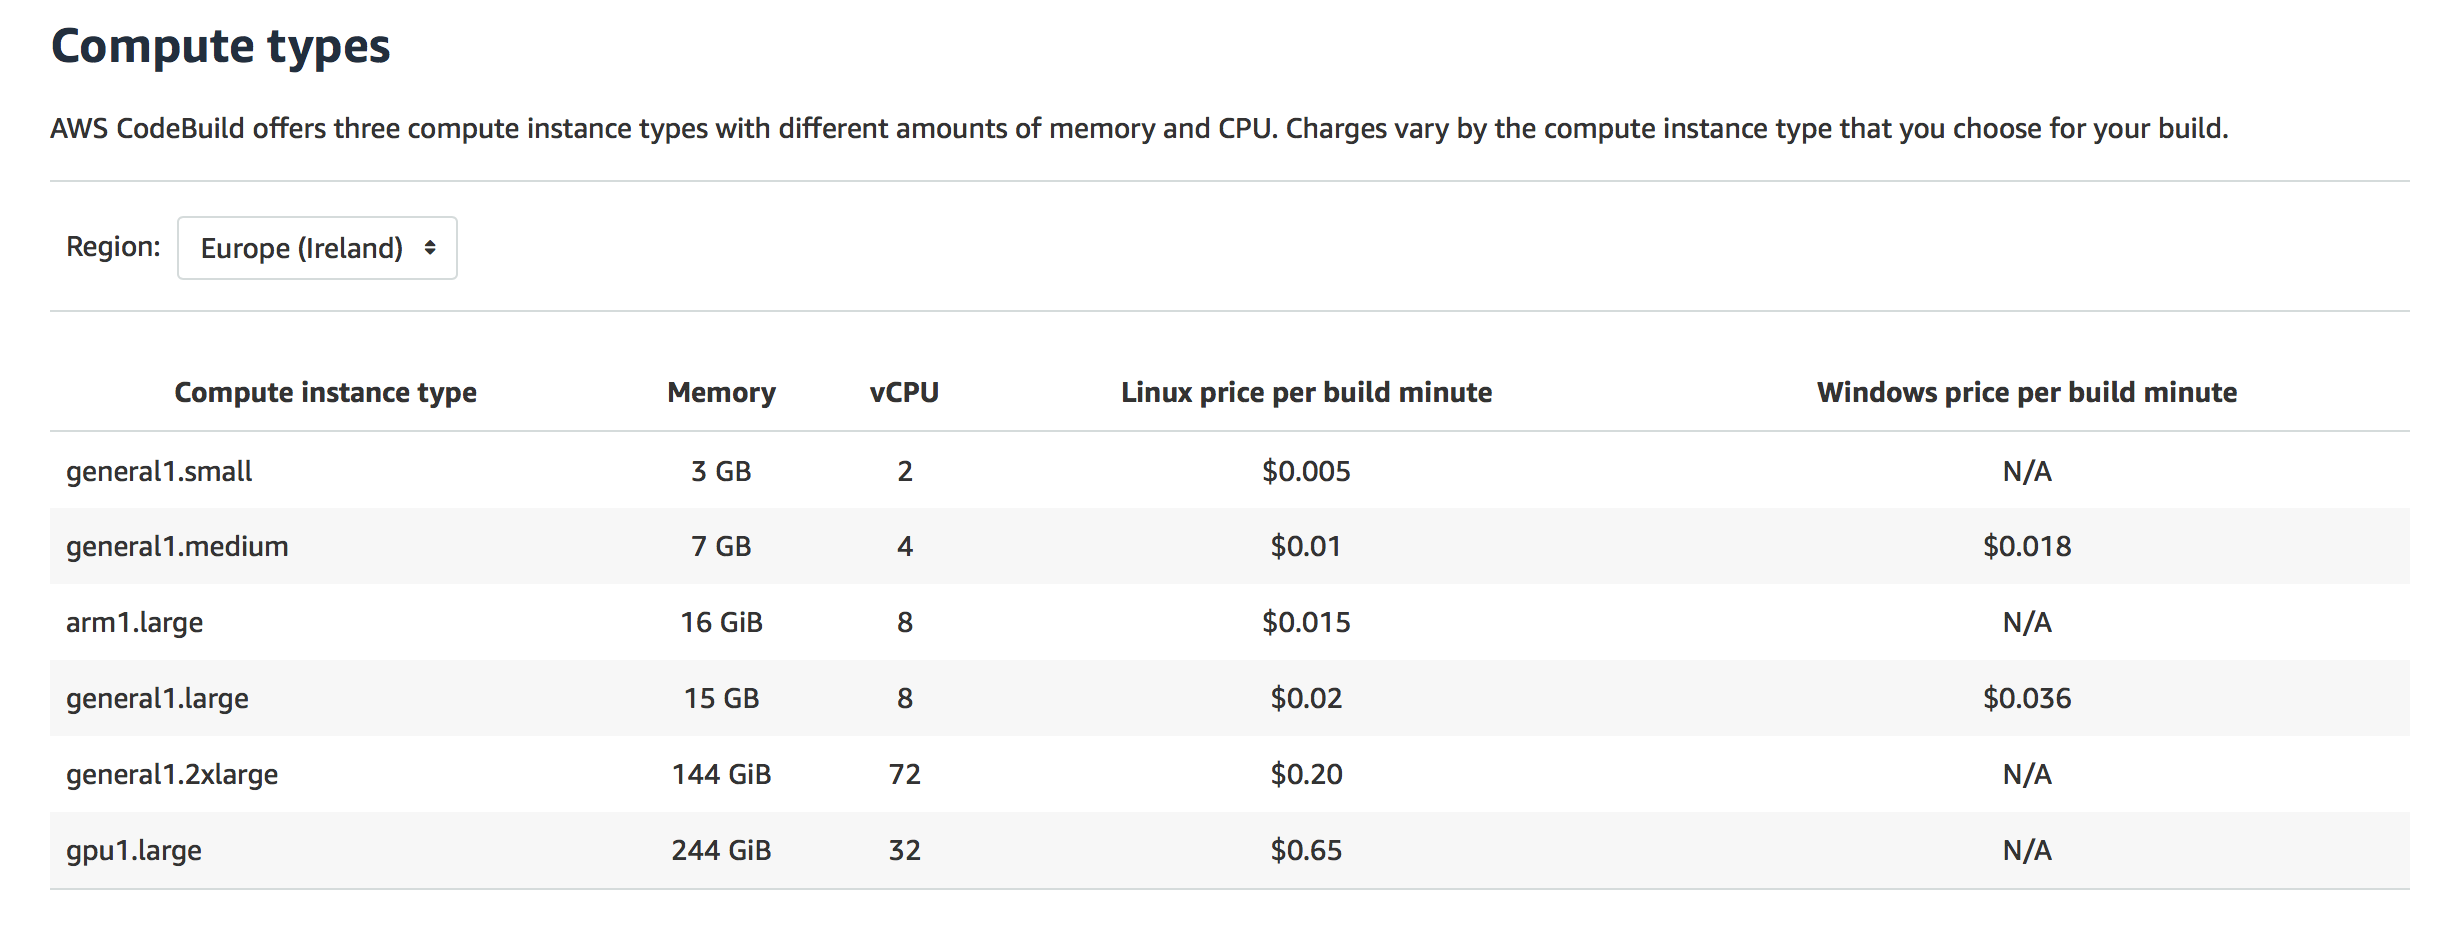
\includegraphics[width=\linewidth]{/Users/kenzie/Documents/HoGent/Bachelorproef/Images/AWS_CB_money.png}
    \caption{Figuur van \href{}{AWS website}. Figuur toont de prijzen van AWS per rekenkracht, OS en verstreken minuut.}
    \label{fig:AWS_CB_money}
\end{figure}
\begin{figure}[!htbp]
    \centering
    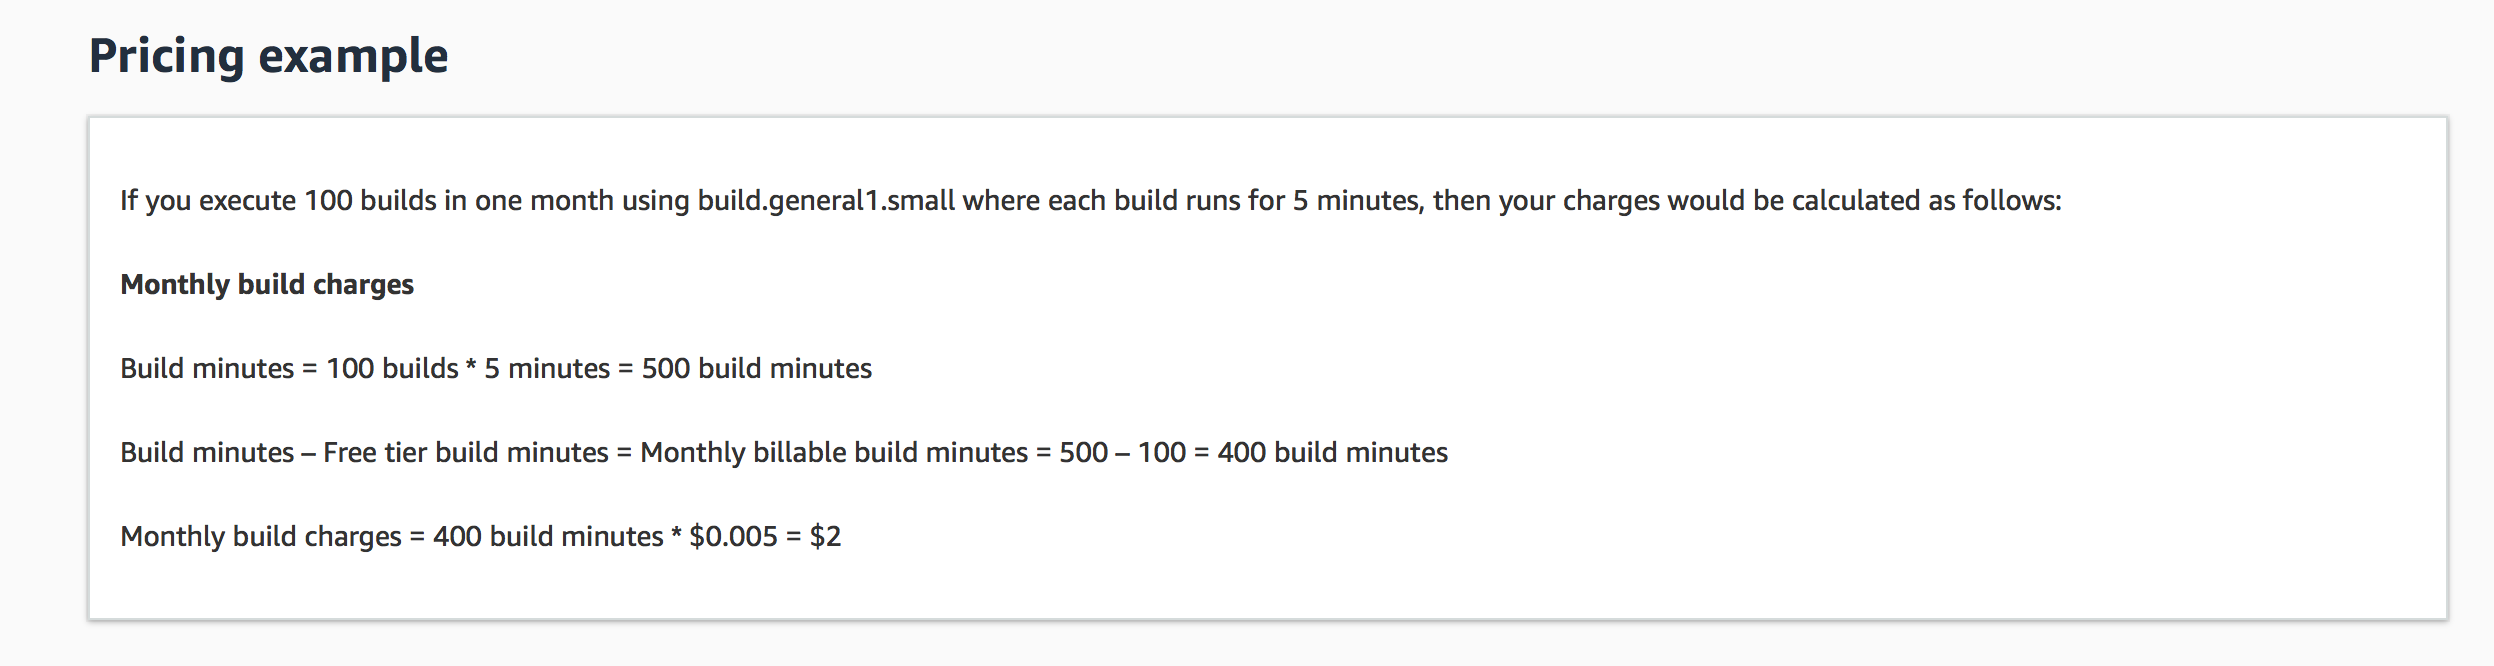
\includegraphics[width=\linewidth]{/Users/kenzie/Documents/HoGent/Bachelorproef/Images/AWS_CB_money2.png}
    \caption{Figuur van \href{}{AWS website}. Figuur toont berekening van prijzen per compileer minuut voor AWS.}
    \label{fig:AWS_CB_money2}
\end{figure}

Een klein detail dat maar zichtbaar was bij het bekijken van de prijzen stelsels. De gebruiker heeft de mogelijkheid om een besturingssysteem (OS) te kiezen bij het aanmaken van een AWS CodeBuild pijpleiding. Dit onderzoek heeft vastgesteld dat een Windows OS wel beschikbaar is maar niet in iedere datacenter locatie. Vaak is die optie ook duurder dan de Linux variant. Dit kan eventueel problemen veroorzaken met Windows specifieke voorbeelden. Ook is het moeilijk om informatie te vinden over hoe de gebruiker nu juist zelf een aangepaste compilatie motor definieert. 

AWS CodeDeploy is het CD gedeelte van de AWS CodePipeline. Het is volledige te beheren en aanpasbaar naar de noden van de gebruiker. Zo is het mogelijk om rechtstreeks vanuit de pijpleiding uit te rollen naar eender welke Amazon Cloud service of naar lokale omgevingen. Aangezien het mogelijk is om een zip met de software in te downloaden is het ook gemakkelijk te integreren met bestaande uitrol tools of werkwijzen. Deze feature is ook niet gratis. Volgende figuur~\ref{fig:AWS_CD_money} toont dit aan. Amazon rekent per update van een instantie een prijs aan. Daarbovenop moet er ook nog betaald worden voor de verbruikte opslag.

\begin{figure}[!htbp]
    \centering
    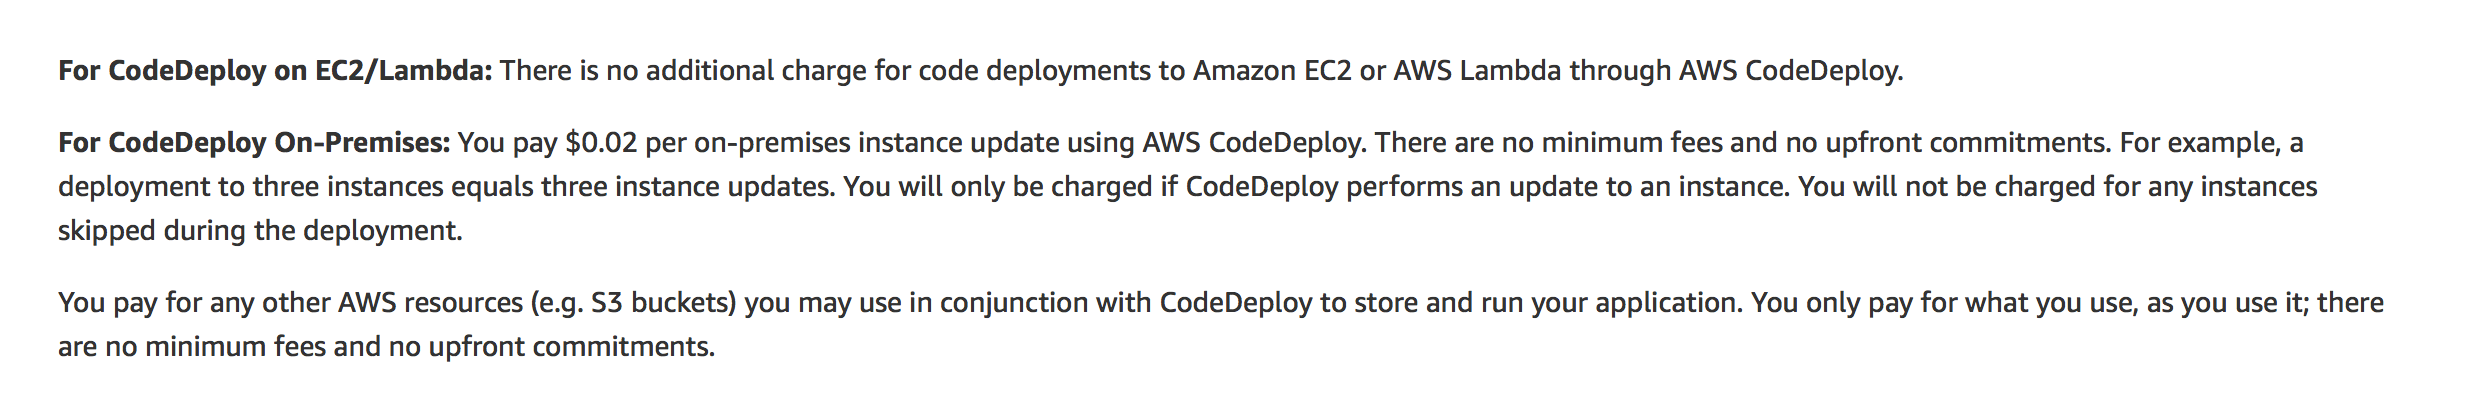
\includegraphics[width=\linewidth]{/Users/kenzie/Documents/HoGent/Bachelorproef/Images/AWS_CD_money.png}
    \caption{Figuur van \href{}{AWS website}. Figuur toont prijs voor opslag op AWS.}
    \label{fig:AWS_CD_money}
\end{figure}

Naast een hele serie ontwikkeltools heeft Amazon ook tools toegevoegd om gedetailleerde rapporten en analyses te genereren van de uitgevoerde taken op AWS CodePipeline. Dit geeft juist zoals Google, de gebruiker goede inzichten in wat er juist allemaal gebeurt en verkeerd loopt. Ook kan de gebruiker op basis van foutmeldingen of status rapporten bepaalde acties instellen en laten uitvoeren.

Het zou mogelijk zijn om met AWS de gewilde functionaliteit de realiseren. Het zal wel zeer arbeid intensief zijn aangezien informatie over zelf een compilatie motor maken moeilijk te vinden is. Ook is het een stuk duurder. Dit onderzoek heeft ook vastgesteld dat Amazon een hele reeks van producten heeft waardoor het soms moeilijk is om door het bos de bomen te zien. Ook de prestatie van het platform blijft een vraagteken door de paper \autocite{Jackson2010}.

\subsection{IBM Cloud}
IBM Cloud is mogelijk een van de oudere Cloud platformen. Voor dat de term Cloud veel gebruikt was. IBM was al vroeg bezig met het idee om hardware open te stellen om dan meerdere machines of services op te laten draaien. In 1972 heeft IBM de eerste stappen gezet naar IaaS door voor hun mainframe een hypervisor te bouwen die toestond dat er meerdere instanties van een besturingssysteem op hetzelfde systeem draaide (VM’s). Dit is dan later geëvolueerd naar een meer typische Cloud infrastructuur. IBM heeft in de vroege jaren van hun Cloud systeem vooral hardware voorzien aan klanten. De zo genoemde privé Cloud. In 2007 werden dan de eerste stappen gezet naar de typisch Cloud infrastructuur door de verhuur van rekenkracht vanuit hun datacenters met hun hardware. 

Heden ten dage is IBM Cloud een stuk uitgebreider. Het valt onder te verdelen in 3 grote categorieën. SmartCloud Foundation, SmartCloud Services en SmartCloud Solutions. Volgens IBM is het hun bedoeling om de gaten in het aanbod van andere Cloud platform aanbieders op te vullen.

SmartCloud Foundation is een serie producten die privé Cloud en Hybride Cloud mogelijk moeten maken. Het biedt de infrastructuur, beheer, beveiliging, hardware en integratie aan. SmartCloud Services zijn dan de verschillende tools om dit te bereiken of te gebruiken. Dus Iaas of PaaS. SmartCloud Solutions is dan meer een pakket dat samenwerking, statistieken enz. moet mogelijk maken binnen de services en aanbiedingen van IBM.

Ook IBM Cloud heeft producten om een CI/CD pijpleiding te maken. Al is er toch een addertje onder het gras. IBM Cloud voorziet infrastructuur om vooral aan CD te kunnen voldoen. Dit met mogelijkheden om de infrastructuur te definiëren. Tools om de uitrol te beheren en te analyseren. Dit alles kan gecontroleerd worden, zoals alle andere Cloud platform aanbieders, door middel van een speciaal ontwikkelde command line interface (CLI) of door hun web portaal. Voor CI biedt IBM niks specifiek aan. Er bestaat wel de mogelijkheid om het Tekton framework te gebruiken op de Cloud infrastructuur van IBM maar dat kan bij iedere Cloud platform aanbieder. Dit valt ook buiten de scope van dit onderzoek.

Op basis van hun producten en services die ze aanbieden valt IBM Cloud uit de boot. Het zou zeer omslachtig zijn om IBM Cloud te gebruiken voor een Microsoft georiënteerde pijpleiding. Aangezien er geen specifieke compilatie technieken aanwezig zijn. Naast het Tekton framework. Ook is de prestatie van de IBM-datacenters niet slecht. Het zijn speciaal ontworpen centers met IBM eigen hardware en voorzieningen. Wat wel blijkt uit onderzoek van de ontwikkeltools van IBM Cloud, is dat IBM zich inzet om gemakkelijk te gebruiken tools te ontwikkelen die weinig moeite kosten om te implementeren en te configureren. Ook hebben ze als enige specifiek een Cloud aanbod voor Apple georiënteerde applicaties.

\subsection{Andere}
Naast de alom bekende giganten zoals Azure, Google Cloud, IBM Cloud en AWS zijn er nog een aantal andere Cloud platform aanbieders. Zo bestaat er nog Oracle Cloud en Digital Ocean. Er bestaan waarschijnlijk nog wel maar deze laat dit onderzoek buiten beschouwing.

Oracle Cloud zijn aanbod van producten en services liggen vooral in vier categorieën. IaaS, PaaS, Software as a Service (SaaS) en Data as a Service. Oracle Cloud hun aanbod is hoofdzakelijk hetzelfde als alle andere Cloud aanbieders. Juist zoals IBM Cloud heeft Oracle hun eigen hardware en eigen datacenters. Oracle Cloud biedt oplossingen en producten aan om DeVops te realiseren maar deze zijn vooral gefocust op het Java platform. Om deze reden valt ook Oracle Cloud uit de boot. Aangezien we in dit onderzoek trachten om een Microsoft georiënteerde pijpleiding willen realiseren. Het is wel mogelijk door gebruik te maken van het Tekton Framework. Maar dit laten we buiten beschouwing in dit onderzoek.

Digital Ocean is een Cloud platform speciaal gemaakt voor ontwikkelaars. Het Cloud platform is een van de jongere aanbieders. Digital Ocean is opgericht in 2011. Hun doel is om een omgeving aan te bieden aan ontwikkelaars waarin programmeurs gemakkelijk kunnen ontwikkelen en testen. Ook tracht Digital Ocean om deze omgeving open te stellen voor productie door het zeer gemakkelijk te maken om services en applicatie schaalbaar te maken op hun platform. Digital Ocean heeft jammer genoeg geen specifiek CI/CD aanbod. Het zou wel mogelijk zijn met het Tekton framework aangezien Digital Ocean Kubernetes ondersteund. Voor deze redenen valt Digital Ocean ook buiten de boot.

\subsection{Kandidaat}
Na al deze Cloud platform aanbieders hun aanbod naast elkaar te hebben gelegd, is er toch een platform dat er wat van tussen uitspringt. Dit is GCP. Daarom is deze Cloud aanbieder ook gekozen in dit onderzoek om een proof of concept op uit te werken. Google is niet alleen een stuk goedkoper, het gebruikt ook simpele en gemakkelijk te gebruiken containers. Ook is het een voordeel dat er gemakkelijk rechten kunnen aangemaakt worden op basis van de GitHub deelnemers. Google heeft ook de meest duidelijke informatiebronnen. Ook zijn het hypermoderne datacenters die over heel de wereld verspreid zijn. Dus prestatie zou geen probleem mogen zijn. Zie figuur~\ref{fig:GCP_NetwerkKaart}.

\begin{figure}[!htbp]
    \centering
    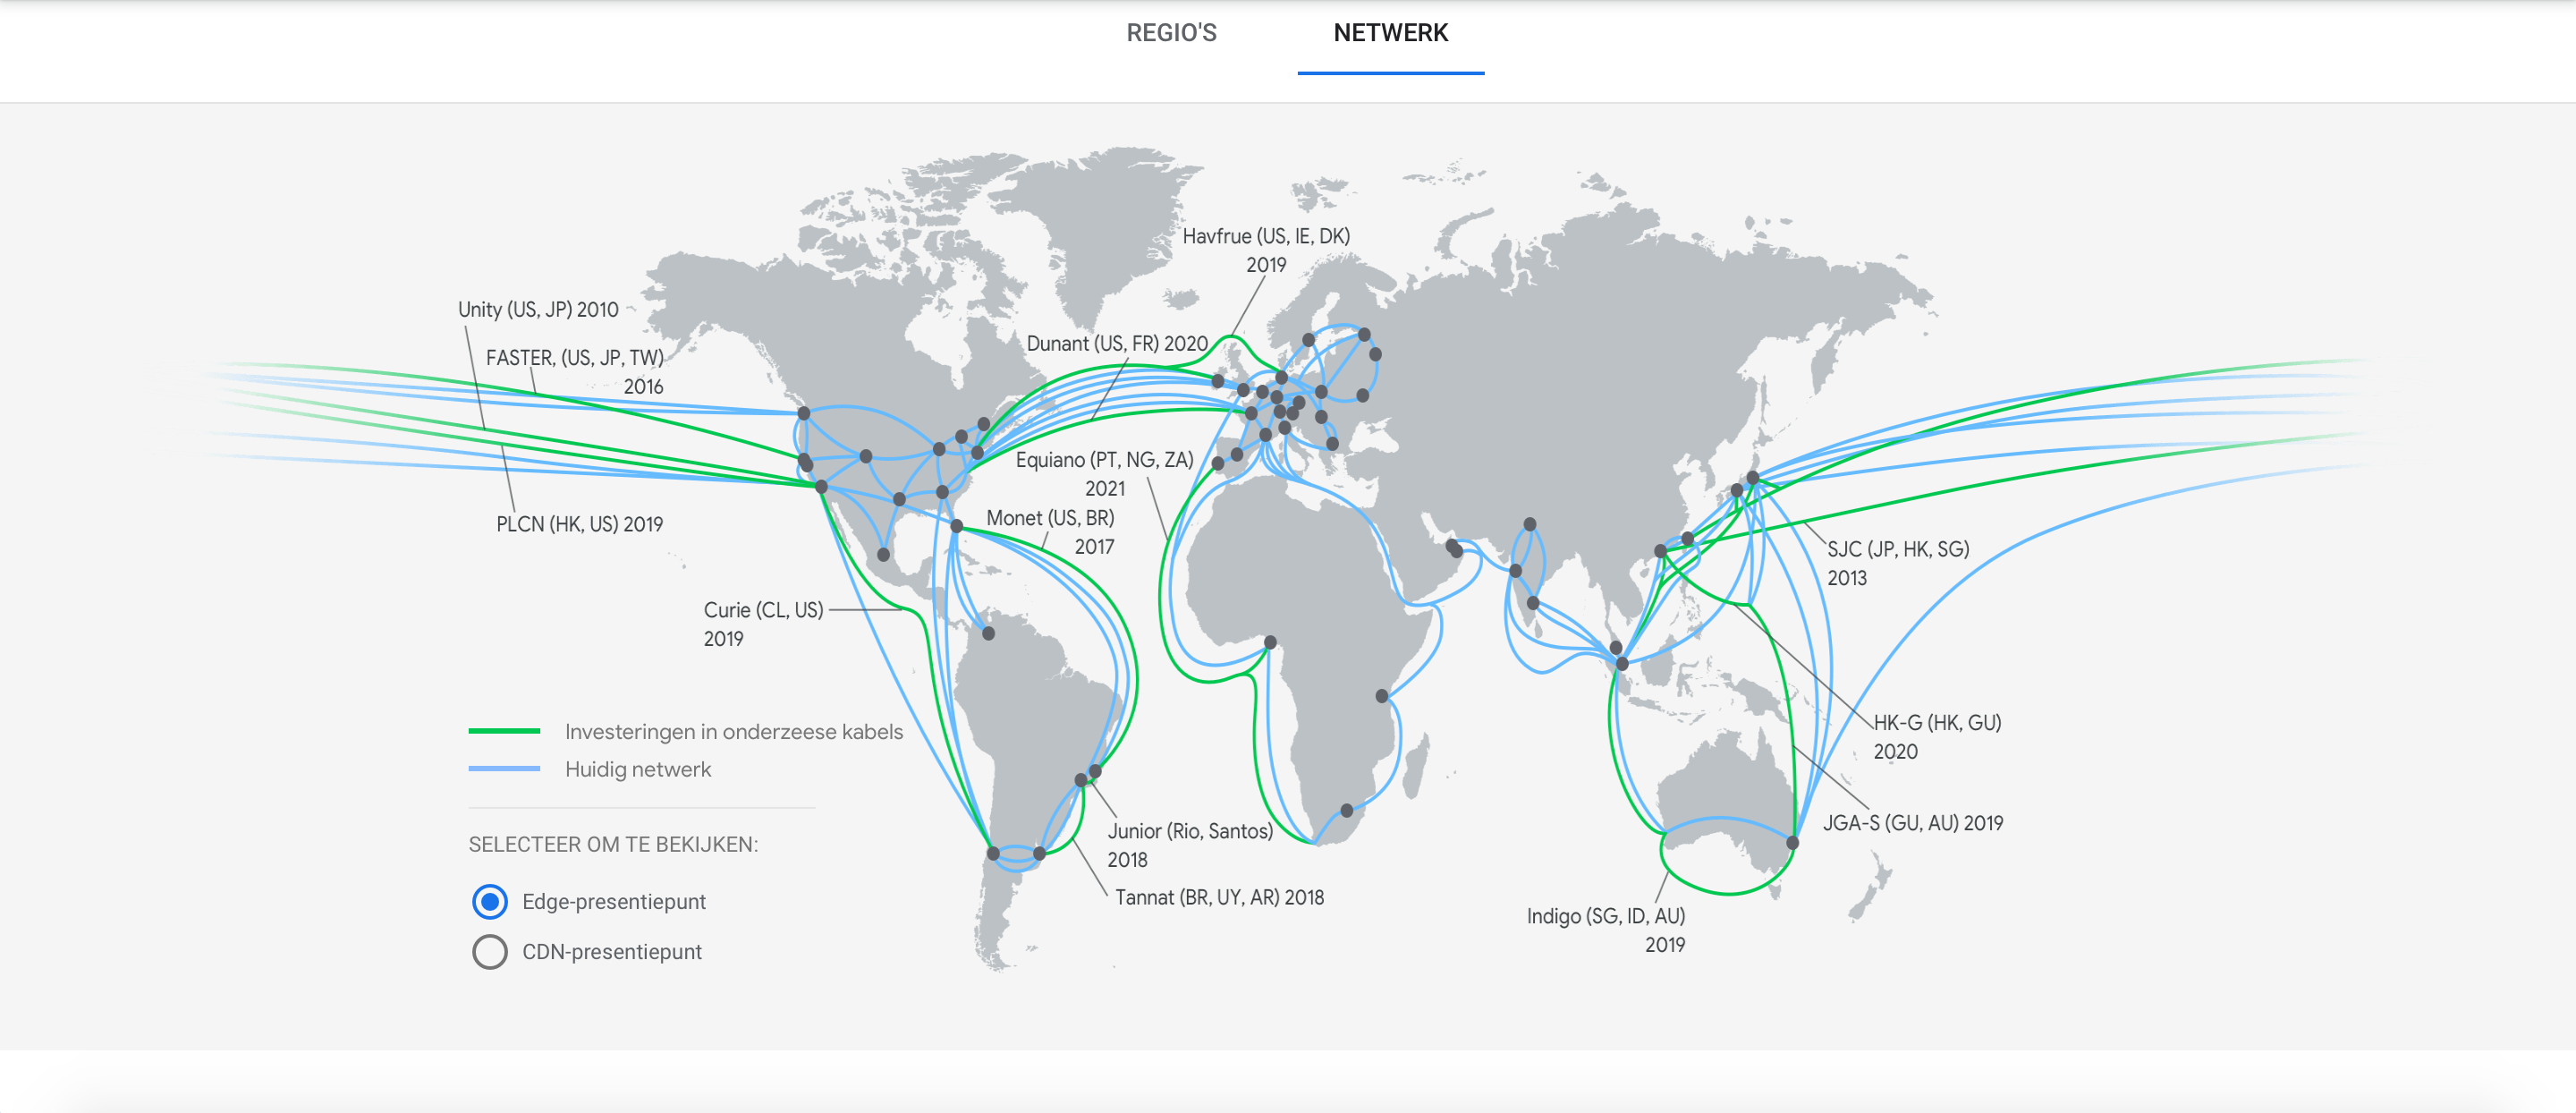
\includegraphics[width=\linewidth]{/Users/kenzie/Documents/HoGent/Bachelorproef/Images/GCP_NetwerkKaart.png}
    \caption{Figuur van \href{}{Google Cloud website}. Figuur toont de connectiviteit van de verschillende datacenters verspreid over de wereld.}
    \label{fig:GCP_NetwerkKaart}
\end{figure}

\section{Kandidaat Selectie}
\label{sec:KandidaatSelectie}
Naast de kandidaat selectie op productaanbod en prijs, wil dit onderzoek ook de gebruiksvriendelijkheid in acht nemen. Hiervoor is er een simpele Java applicatie gebruikt. Alle Cloud platformen bieden starterhandleidingen aan voor het opzetten van een CI-pijpleiding voor Java op hun platform. Het doel van deze snelle test is om als eindresultaat een werkende Java JAR te hebben. Ook werd er bijgehouden hoelang het duurde om een pijpleiding te configureren om beter een idee te krijgen van hoe gebruiksvriendelijk het Cloud platform werkelijk is. 

De Java Applicatie bestaat uit een hoofdklasse en een testklasse. De hoofdklasse, ‘MessageUtil’ bevat een variabele voor een bericht te bewaren en vier methodes. De eerste methode is een constructor voor het aanmaken van een ‘MessageUtil’ object met een meegegeven bericht. De tweede methode print dit bericht. In de derde methode wordt er een toevoegsel aan dit bericht gevoegd. Ook wordt het geheel geprint. De laatste methode is een uitvoerbare methode die een ‘MessageUtil’ object maakt en de twee print methodes uitvoert. De code voor ‘MessageUtil.java’ wordt afgebeeld in \emph{figuur~\ref{code:messageutilj}}. 

De testklasse ‘TestMessageUtil’ bevat twee testen voor de print methodes. \emph{Figuur~\ref{code:messageutiltestj}}  toont de code voor dit Javabestand.

\lstset{
    language=java,
    breaklines=true,
    frame=single,
    commentstyle=\color{mygreen},
    keywordstyle=\color{blue},
    numberstyle=\tiny\color{mygray},
    stringstyle=\color{mymauve},
    captionpos=b,
    caption={Java bestand MessageUtil.java. Hoofd klasse van de applicatie \emph{MessageUtil}},
    label=code:messageutilj
}
\begin{lstlisting}
public class MessageUtil {
private String message;

    public MessageUtil(String message) {
        this.message = message;
    }

    public String printMessage() {
        System.out.println(message);
        return message;
    }

    public String salutationMessage() {
        message = "Hi!" + message;
        System.out.println(message);
        return message;
    }
    
    public static void main(String[] args) {
        MessageUtil mu = new MessageUtil("Idioten zijn er overal...");
        mu.printMessage();
        mu.salutationMessage();
    }
}
\end{lstlisting}

\lstset{
    language=java,
    caption={Java Test klasse MessageUtilTest.java, voor het testen van \emph{MessageUtil~\ref{code:messageutilj}}.},
    label=code:messageutiltestj
}
\begin{lstlisting}
import org.junit.Test;
import org.junit.Ignore;
import static org.junit.Assert.assertEquals;

public class TestMessageUtil {

    String message = "Robert";    
    MessageUtil messageUtil = new MessageUtil(message);

    @Test
    public void testPrintMessage() {      
        System.out.println("Inside testPrintMessage()");     
        assertEquals(message,messageUtil.printMessage());
    }

    @Test
    public void testSalutationMessage() {
        System.out.println("Inside testSalutationMessage()");
        message = "Hi!" + "Robert";
        assertEquals(message,messageUtil.salutationMessage());
    }
}
\end{lstlisting}

Deze Javabestanden worden op alle Cloud platformen gecompileerd aan de hand van de Maven compiler. Om de compiler te vertellen wat er moet gebeuren tijdens de compilatie van de Javabestanden, moet er een Xml-bestand aangemaakt worden waarin deze opties gedefinieerd staan. Deze ‘pom.xml’ wordt afgebeeld door \emph{figuur~\ref{code:pom}}. Hierin staat dat de meegeleverde Junit testen uitgevoerd moeten worden. Ook wordt er gedefinieerd dat de Java applicatie moet gecompileerd worden tot een JAR-bestand.

\lstset{
    language=XML,
    caption={XML-bestand voor de Maven compiler. Definieert stappen voor het compileren van een java applicatie.},
    label=code:pom
}
\begin{lstlisting}
<project xmlns="http://maven.apache.org/POM/4.0.0" 
        xmlns:xsi="http://www.w3.org/2001/XMLSchema-instance"
        xsi:schemaLocation="http://maven.apache.org/POM/4.0.0 http://maven.apache.org/maven-v4_0_0.xsd">
    <modelVersion>4.0.0</modelVersion>
    <groupId>org.example</groupId>
    <artifactId>messageUtil</artifactId>
    <version>1.0</version>
    <packaging>jar</packaging>
    <name>Message Utility Java Sample App</name>
    <dependencies>
        <dependency>
            <groupId>junit</groupId>
            <artifactId>junit</artifactId>
            <version>4.11</version>
            <scope>test</scope>
        </dependency>	
    </dependencies>
    <build>
            <plugins>
                <plugin>
                    <groupId>org.apache.maven.plugins</groupId>
                    <artifactId>maven-jar-plugin</artifactId>
                    <version>3.1.0</version>
                    <configuration>
                        <archive>
                            <manifest>
                                <addClasspath>true</addClasspath>
                                <classpathPrefix>lib/</classpathPrefix>
                                <mainClass>MessageUtil</mainClass>
                            </manifest>
                        </archive>
                    </configuration>
                </plugin>
            </plugins>
    </build>
</project>
\end{lstlisting}

Deze bestanden zijn toegevoegd aan een folder die de structuur hanteert uit \emph{figuur~\ref{code:treejava}}. Deze hoofdmap is dan geïnitialiseerd als een Git repositorie. Ook is er een gitignore aangemaakt. Deze Java applicatie is het startpunt voor alle testen voor gebruiksvriendelijkheid op de Cloud platformen. Op deze manier is er geprobeerd om op basis van eventuele verschillen een geschikte kandidaat te selecteren voor een Proof Of Concept. In de volgende secties~\ref{sec:JAA}, ~\ref{sec:JGCP} \& ~\ref{sec:JAD} wordt kort de werkwijze beschreven. Hier wordt de ‘hoe’ minder aangehaald omdat dit in de handleiding beschreven staat.

\lstset{
    language=bash,
    caption={Output van het tree commando in een java applicatie bestanden structuur.},
    label=code:treejava
}
\begin{lstlisting}
Demo_java_aws/
`--- .gitignore
`--- pom.xml
`--- src
    `--- main
        `--- java
           `--- MessageUtil.java
    `--- test
        `--- java
           `--- TestMessageUtil.java
\end{lstlisting}

\subsection{Java Amazon AWS}
\label{sec:JAA}


\subsection{Java Google Cloud Platform}
\label{sec:JGCP}

\subsection{Java Azure DeVops}
\label{sec:JAD}

\section{Proof Of Concept}
\label{sec:POC}
Omdat Aucxis met een Microsoft georiënteerde werkwijze zit, moet er worden aangetoond dat het mogelijk is om dit te realiseren op GCP. Voor deze Proof Of Concept (POC) wordt er een CI/CD pijpleiding geconfigureerd. Hierin wordt er een simpele .NET Core applicatie gecompileerd. Ook de meegeleverde testen worden uitgevoerd tijdens de compilatie. Hierna wordt de applicatie en de bijbehorende componenten gecomprimeerd en naar een lokale fileserver geüpload. De gecompileerde applicatie kan dan uitgebreid getest worden in een lokale test omgeving. Ook is er een stap voorzien in de pijpleiding om de gecompileerde applicatie tijdelijk op het Cloud platform te bewaren. Dit voor het geval er iets verkeerd loopt tijdens het testen of tijdens het uploaden.

De .Net applicatie is een simpele .Net core console applicatie. Het bestaat uit een klasse, \emph{MessageUtil~\ref{code:messageutil}}. Deze klasse bevat een variabele, twee constructors, een methode om de variabele op te vragen, een methode om de variabele te tonen met een toevoegsel en een hoofdmethode die uitvoerbaar is.

\lstset{
     language=C,
     breaklines=true,
     frame=single,
     commentstyle=\color{mygreen},
     keywordstyle=\color{blue},
     numberstyle=\tiny\color{mygray},
     stringstyle=\color{mymauve},
     captionpos=b,
     caption={C\# bestand MessageUtil.cs. Hoofd klasse van de applicatie \emph{MessageUtil}},
     label=code:messageutil
}
\begin{lstlisting}
using System;
using System.Threading;

namespace MessageUtil {
    public class MessageUtilProgram {
    
        private String p_message;
        
        private MessageUtilProgram() { }
        public MessageUtilProgram(String message) {
            p_message = message;
        }
        
        public String Message {
            get { return p_message; }
        }
        public String SaluteMessage(String m) {
            Console.WriteLine("Hello\n{0}", m);
            return "hello" + m;
        }
        
        static void Main(string[] args) {
            MessageUtilProgram mup = new MessageUtilProgram("Aucxis");
            Console.WriteLine("{0}", mup.Message);
            //mup.SaluteMessage(mup.Message);
            Thread.Sleep(60000);
        }
    }
}
\end{lstlisting}

Daarnaast is er ook een testklasse voorzien, \emph{MessageUtilTest~\ref{code:messageutiltest}}. Hierin staan er twee methodes. De eerste methode test de constructor die de variabele moet instellen. De tweede methode test een van de print methodes.

\lstset{
    language=C,
    caption={C\# Test klasse MessageUtilTest.cs, voor het testen van MessageUtil~\ref{code:messageutil}.},
    label=code:messageutiltest
}
\begin{lstlisting}
using Microsoft.VisualStudio.TestTools.UnitTesting;
using MessageUtil;
    
namespace MessageUtilTest {

    [TestClass]
    public class MessageUtilTests {
    
        [TestMethod]
        public void ConstructWorks() {
            string testmessage = "Test";
            MessageUtilProgram mup = new MessageUtilProgram(testmessage);

            string value = mup.Message;
            Assert.AreEqual(testmessage, value,"Message didn't set correctly");
        }
        
        [TestMethod]
        public void SaluteWorks() {
            string testmessage = "Test";
            string expected = "helloTest";
            MessageUtilProgram mup2 = new MessageUtilProgram(testmessage);

            string value = mup2.SaluteMessage(mup2.Message);
            Assert.AreEqual(expected, value, "Message didn't salute correctly");
        }
    }
}
    
\end{lstlisting}

De applicatie wordt in beide gevallen onveranderd gebruikt zodanig dat een potentieel verschil zichtbaar wordt. Dit is de basis waaruit vertrokken is voor de vergelijkende POC. Om de prijs en het aantal benodigde producten zo laag mogelijk te houden, is er in dit onderzoek gekozen om Git en GitHub te gebruiken als versiebeheersysteem. GitHub is volledig ondersteund door beide platformen. Ook voorzien beide Cloud platformen applicaties op GitHub om automatisch de gewenste repositories te verbinden aan de CI/CD pijpleidingen.

Het uploaden van de gecomprimeerde applicatie wordt gedaan door middel van Secure File Transfer Protocol (SFTP) op een Linux Ubuntu machine. Deze maakt verbinding met een Docker container die lokaal op een Windows Server 2019 draait. Deze\emph{~\href{https://hub.docker.com/r/atmoz/sftp/}{Docker container}} deelt een directory met Windows zodanig dat dit volledig modulair is met andere besturingssystemen of situaties. SFTP werkt onderliggend op basis van Secure Shell (SSH). Om verbinding te maken is dus een wachtwoord nodig. Dit is een probleem aangezien de virtuele systemen in de Cloud niet interactief zijn. Dit is opgelost door het gebruik van\emph{~\href{https://linux.die.net/man/1/sshpass}{SSHPASS}}. Dit Linux pakket heeft de mogelijkheid om aan SSH-toepassingen het wachtwoord mede te geven. Weliswaar zonder encryptie van het wachtwoord. Hierdoor is het wachtwoord leesbaar. Er wordt enkel op deze wijze gewerkt om het geheel relatief simpel te houden. Voor productie omgevingen zou er met SSH-sleutels gewerkt moeten worden. De SFTP operatie op de Linux Ubuntu in de Cloud, wordt uitgevoerd door middel van het \emph{script~\ref{code:filetrans}}. Dit Bash script zorgt ervoor dat het SSHPASS pakket beschikbaar is en voert de SFTP transactie uit.

\lstset{
    language=bash,
    caption={Bash script filetrans.sh. Script installeert de juiste Linux packages en kopieert de bestanden met SFTP.},
    label=code:filetrans
}
\begin{lstlisting}
#! /bin/bash
apt-get update
apt-get -y upgrade
apt-get -y install sshpass
sshpass -p 'pwd' sftp -o StrictHostKeyChecking=accept-new -P 5151 -oBatchMode=no -b - TestU@server << !
cd documents
put /workspace/MessageUtil/bin/Release/netcoreapp3.1/win10-x64/messageutil-win10-x64.tar.gz
bye
!
\end{lstlisting}

De Cloud specifieke configuratie bestanden worden in de volgende secties verder verduidelijkt. Voor GCP in \emph{sectie~\ref{sec:VergelijkingGCP}} en voor het Azure DeVops platform \emph{sectie~\ref{sec:VergelijkingADV}}.

\subsection{Google Cloud Platform}
\label{sec:VergelijkingGCP}
Voor deze POC is er een nieuw project aangemaakt op Google Cloud. Als op Google Cloud een project verwijderd wordt, worden ook alle resources en aanrekeningen stopgezet. Ook omdat er dan per project producten en services toegewezen kunnen worden. Zo kan er optimaal voldaan worden aan de gebruiker zijn noden. Het nieuw gecreëerde project, heeft de naam ‘net-demo-project’ gekregen zoals in \emph{figuur~\ref{fig:GCP_POC_projn}}.

\begin{figure}[!htbp]
    \centering
    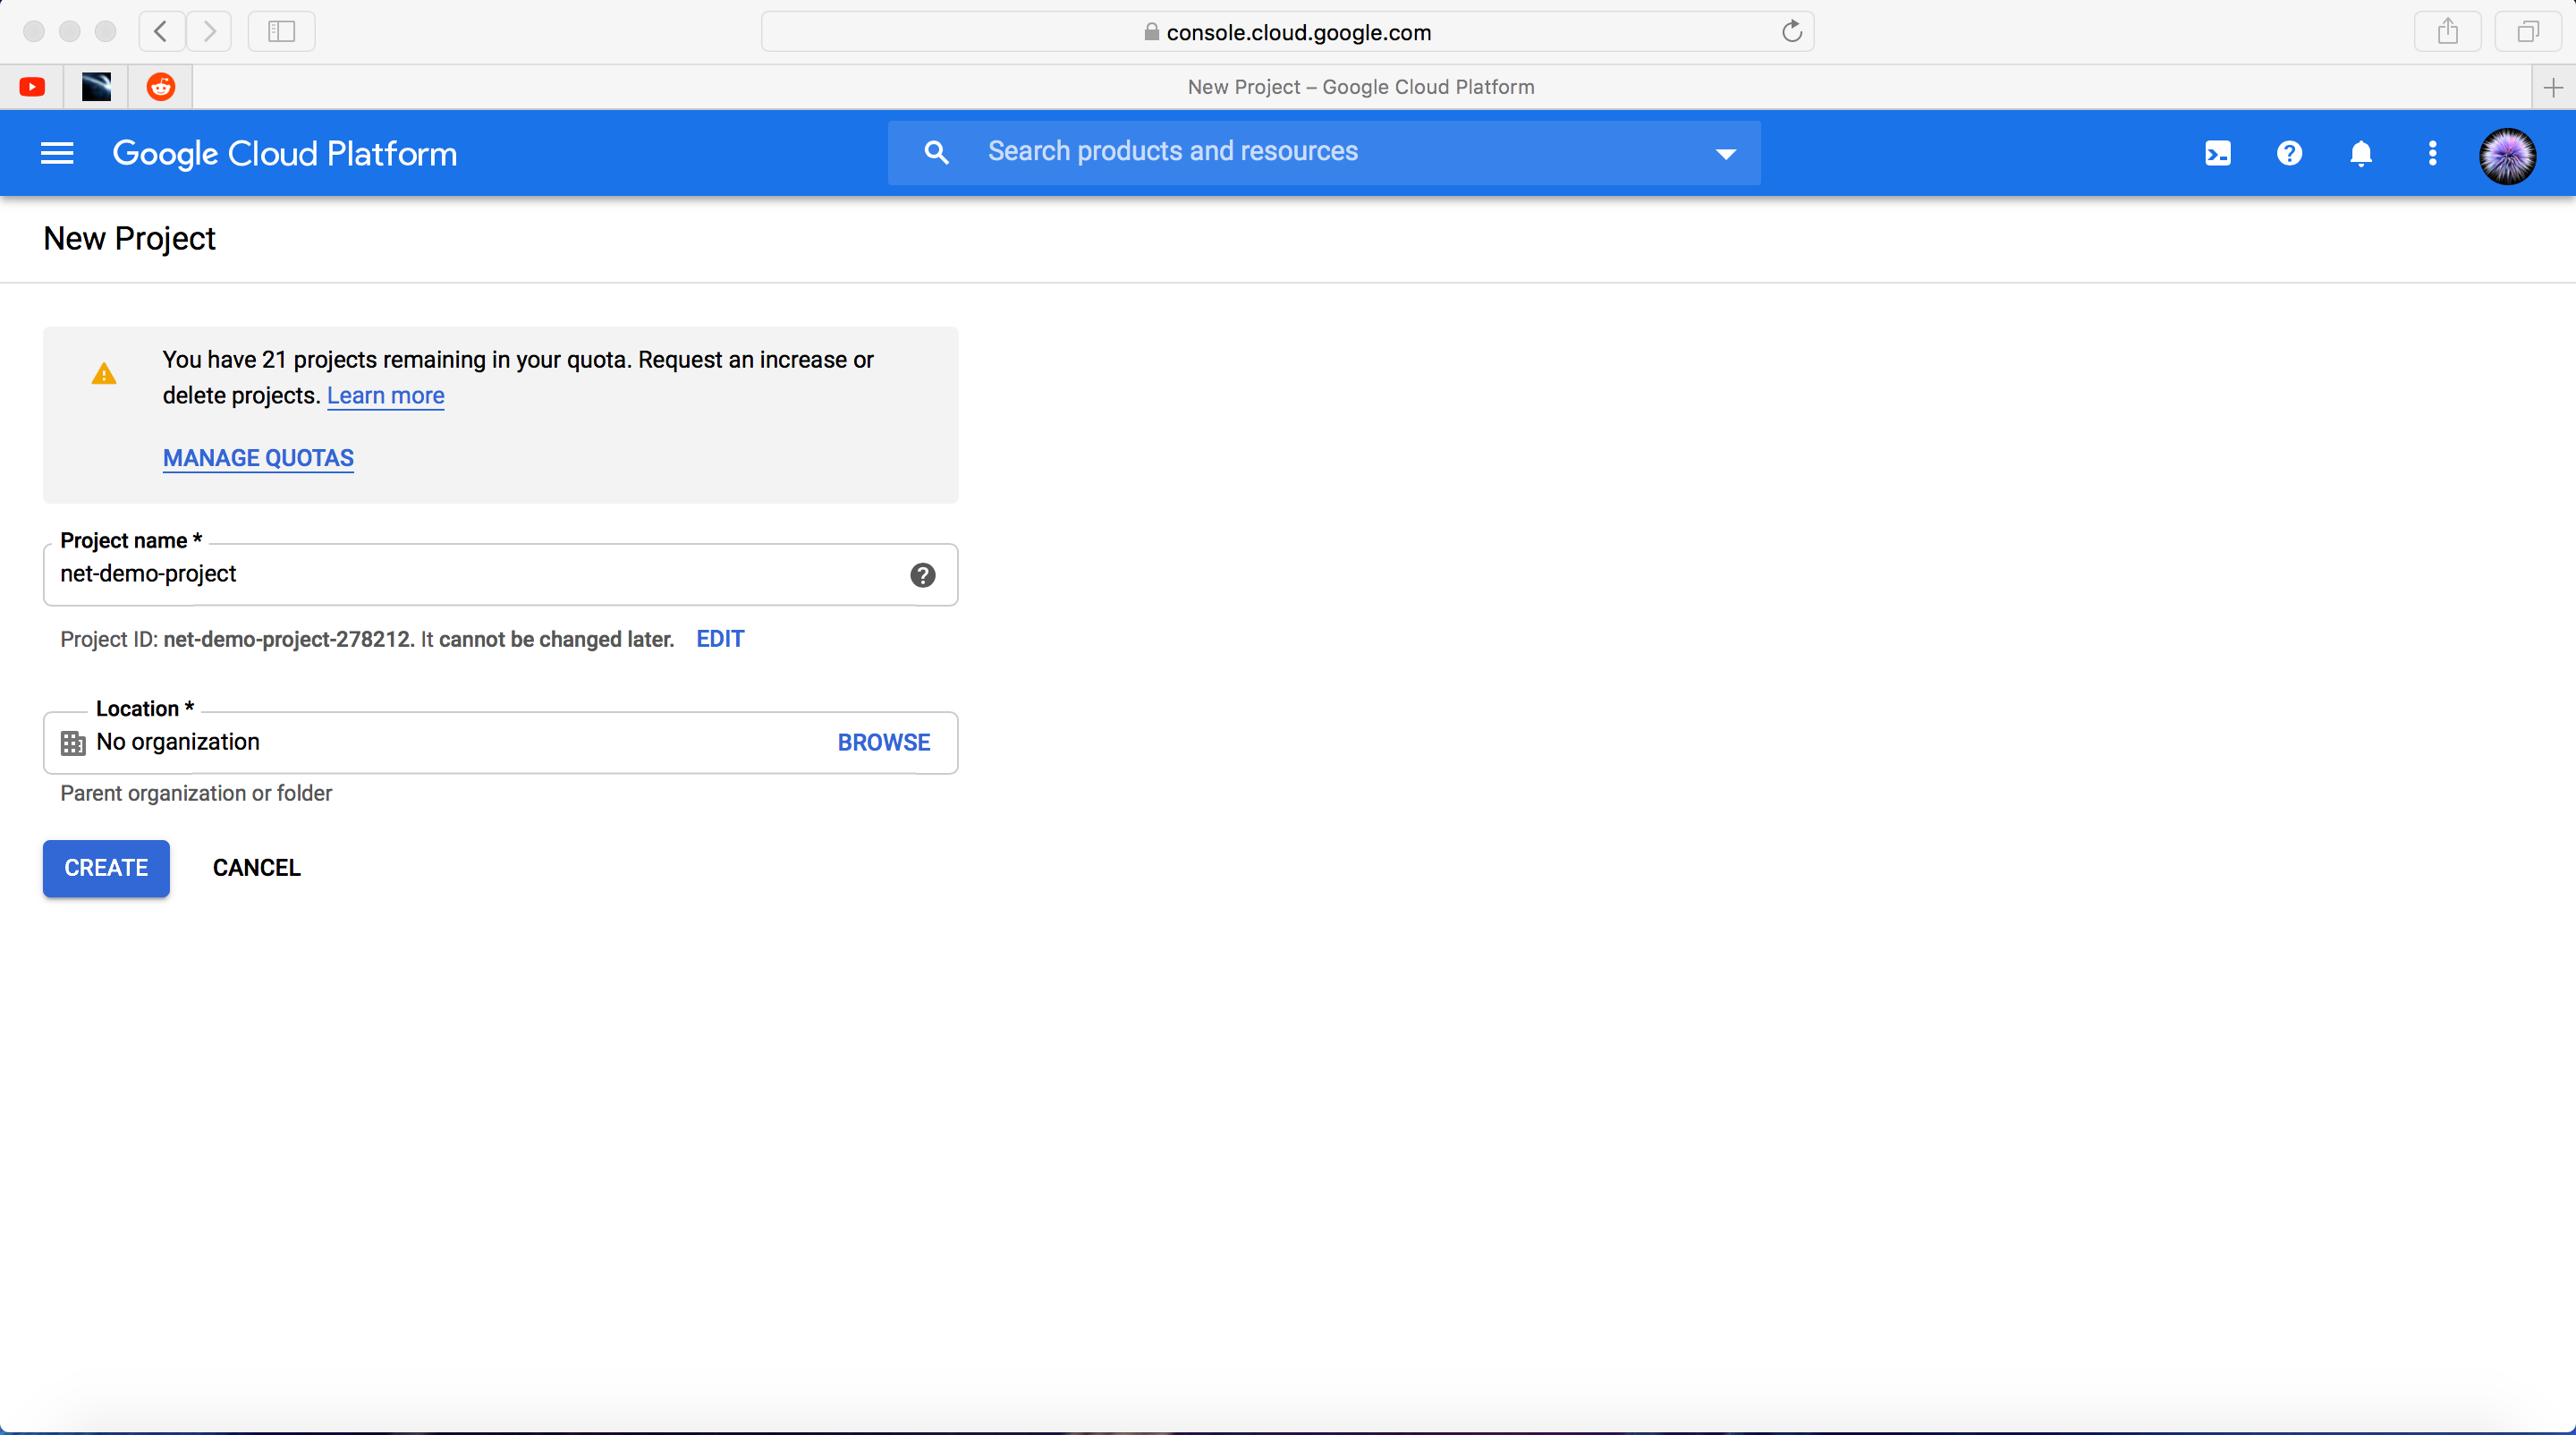
\includegraphics[width=\linewidth]{/Users/kenzie/Documents/HoGent/Bachelorproef/Images/gcp_net_demo_projn.png}
    \caption{Figuur toont het scherm om een nieuw project te creëren op Google Cloud.}
    \label{fig:GCP_POC_projn}
\end{figure}

Om Code Build op Google Cloud te gebruiken moest eerst de API via de online console geactiveerd worden. Ook moest er nog een Storage Bucket aangemaakt worden voor het opslaan van de gecompileerde applicatie. De Storage service is standaard geactiveerd en hoefde dus niet aangezet te worden. Deze Storage Bucket heeft de naam ‘net-demo-output-bucket’ gekregen. Ook belangrijk was de selectie voor de locatie van deze Storage Bucket. Hier is er gekozen voor een geografisch zo dicht mogelijke locatie. Dit om de overdracht tijden van bestanden zo minimaal mogelijk te houden. Alle andere opties zijn onveranderd gebleven. Ook is er de mogelijkheid om toegangsrechten toe te kennen. Dit kan interessant zijn voor een productie omgeving. \emph{Figuur~\ref{fig:GCP_POC_sb}}toont de gecreëerde Storage Bucket en de geselecteerde opties.

\begin{figure}[!htbp]
    \centering
    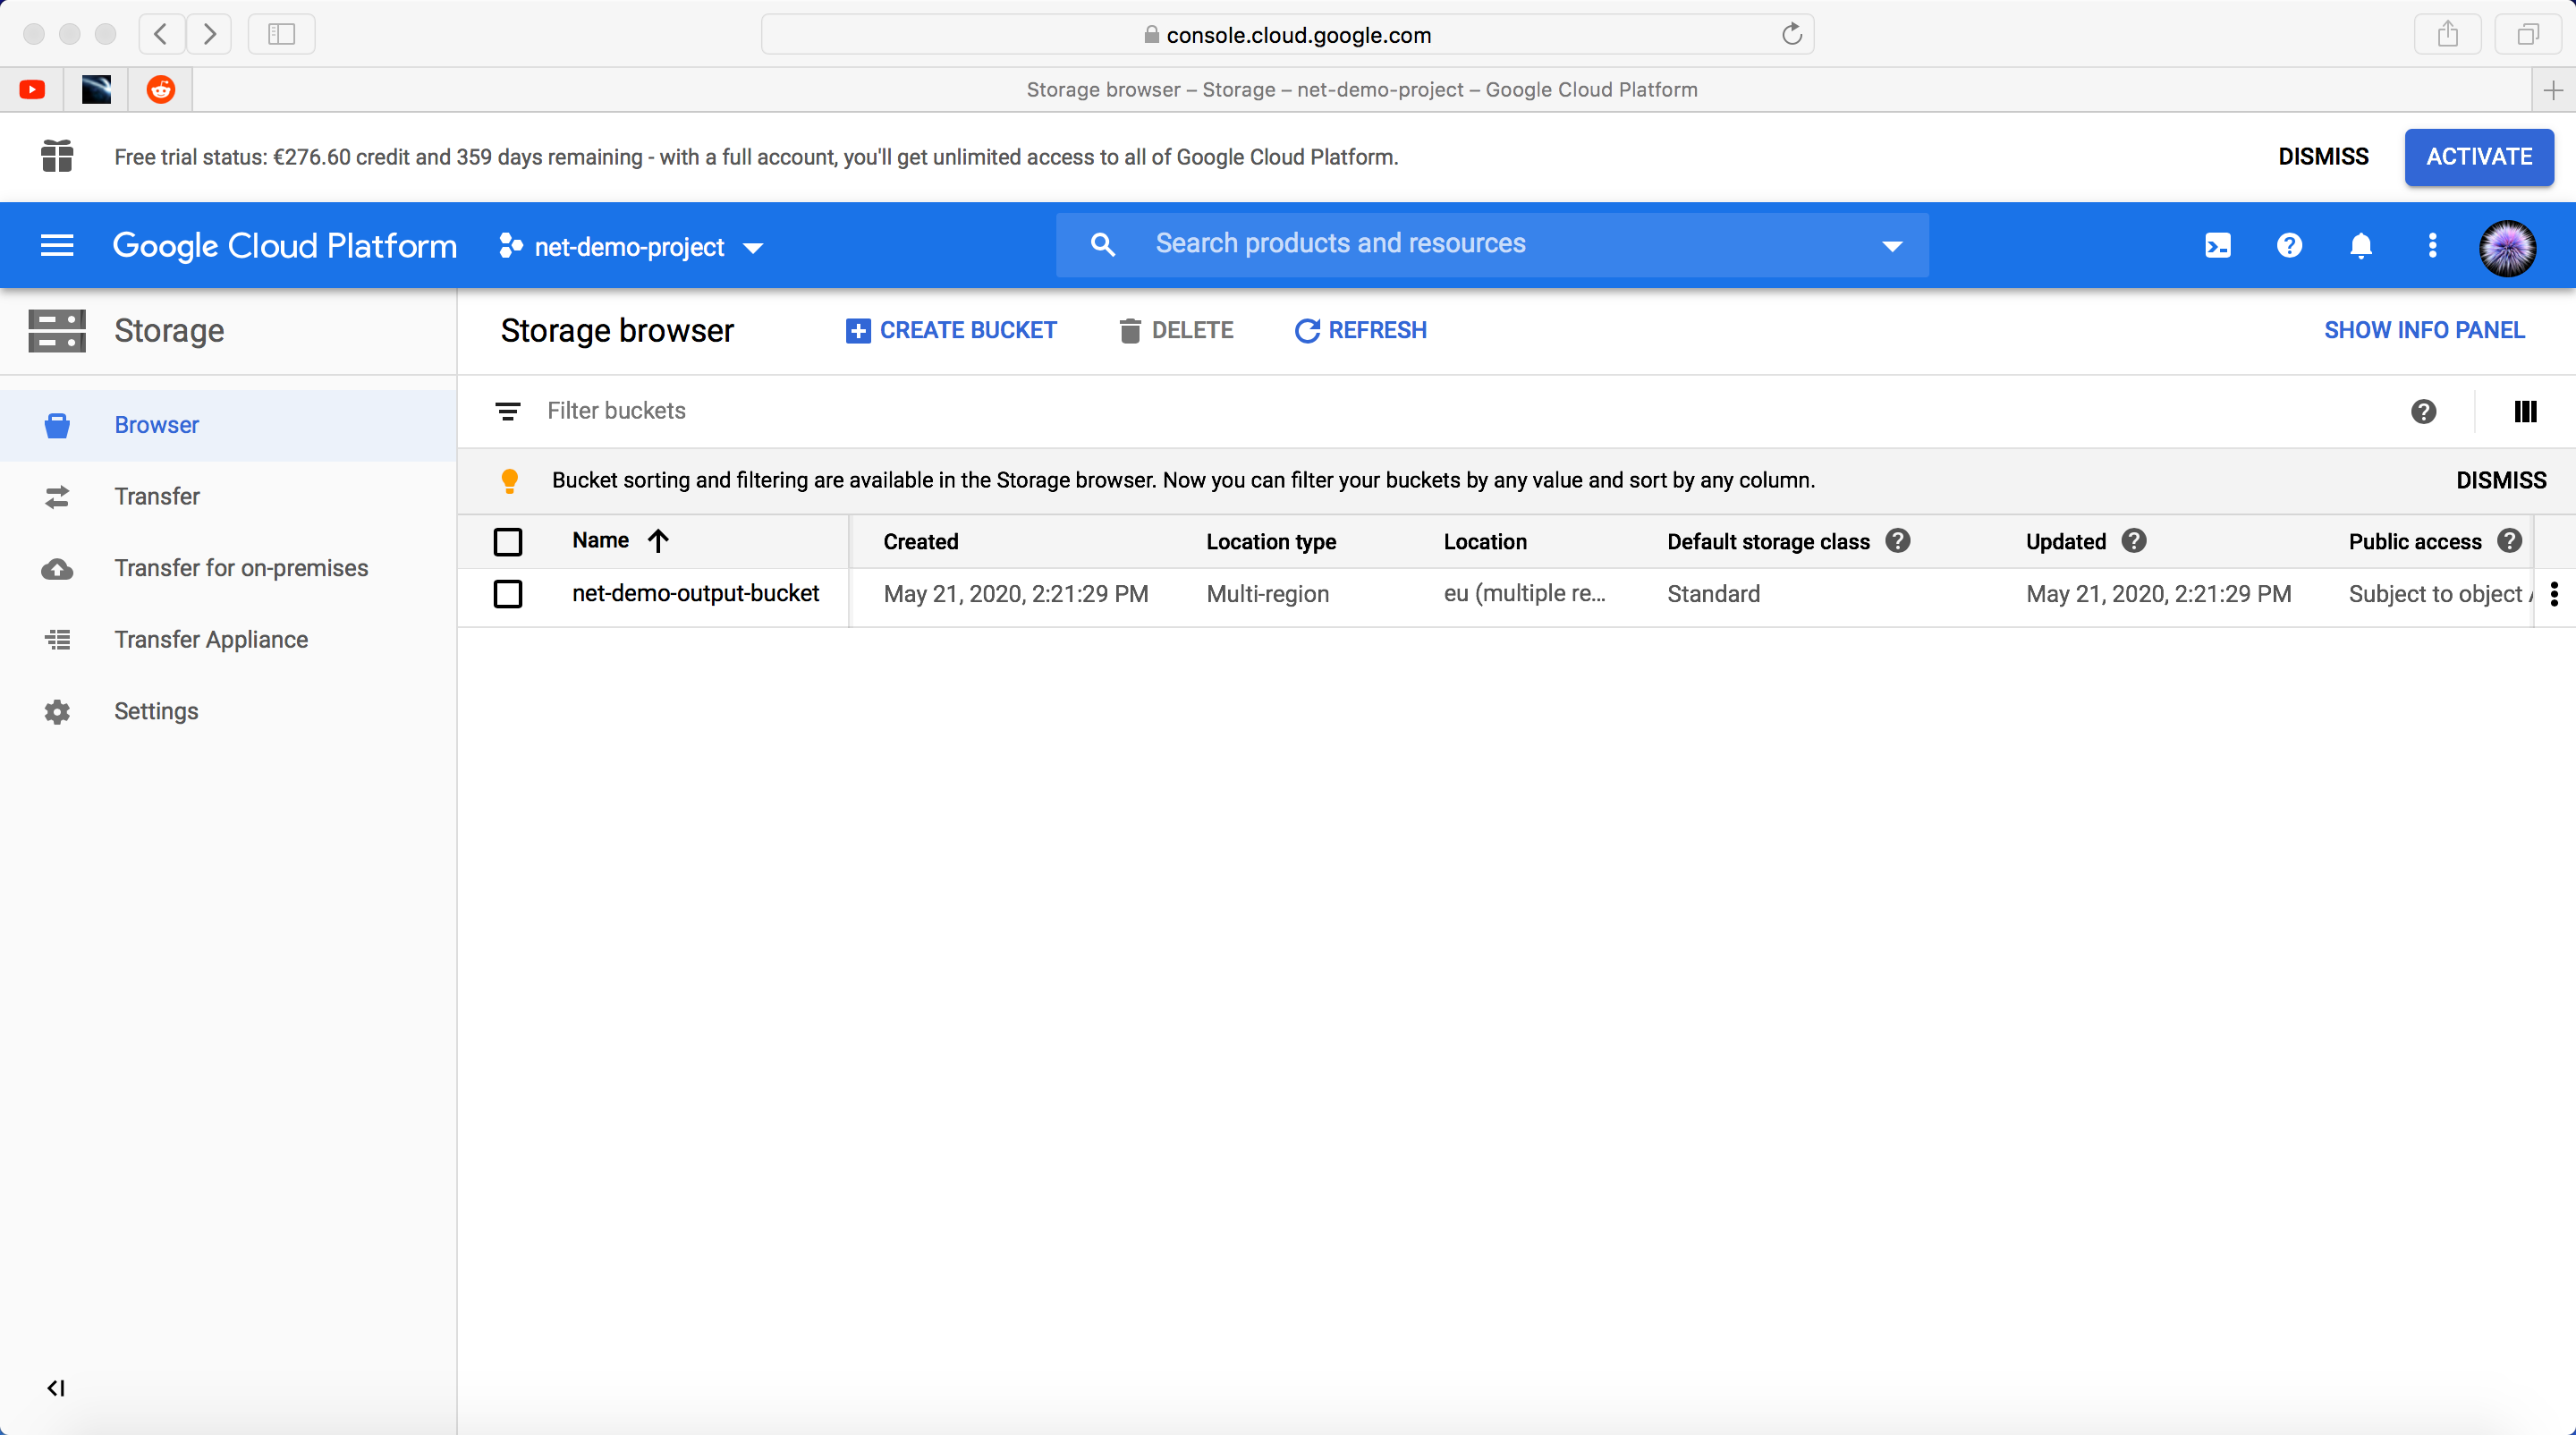
\includegraphics[width=\linewidth]{/Users/kenzie/Documents/HoGent/Bachelorproef/Images/gcp_net_demo_sb.png}
    \caption{Figuur toont het scherm met een gecreëerde Storage Bucket en de geconfigureerde opties op Google Cloud.}
    \label{fig:GCP_POC_sb}
\end{figure}

Hierna is er een nieuwe map aangemaakt op de gebruiker zijn computer voor de applicatie. Deze is geïnitialiseerd als een Git repositorie. Hierin zijn dan de bestanden, \emph{MessageUtil~\ref{code:messageutil}} \& \emph{MessageUtilTest~\ref{code:messageutiltest}} voor de .Net applicatie in geplaatst. Ook het \emph{script~\ref{code:filetrans}} voor de bestanden overdracht met SFTP is hierbij toegevoegd. Hiernaast is er ook een gitignore aangemaakt. \emph{Figuur~\ref{code:gcpgittree}} toont een tree van de bestanden en mappen structuur.

\lstset{
    language=bash,
    caption={Tree van de bestanden structuur voor de Proof Of Concept op Google Cloud.},
    label=code:gcpgittree
}
\begin{lstlisting}
poc_gcp_dotnet/
`--- .git
`--- .gitignore
`--- MessageUtil
      `--- MessageUtil.csproj
      `--- MessageUtilProgram.cs
`--- MessageUtil.sln
`--- MessageUtilTest
      `--- MessageUtilTest.csproj
      `--- MessageUtilTests.cs
`--- filetrans.sh
\end{lstlisting}

Vervolgens moest er connectie gemaakt worden met het gecreëerde project op Google Cloud met Google Cloud CLI. Hiervoor is op de CLI van de gebruiker zijn computer \emph{gcloud init -console only} uitgevoerd. Vervolgens is de wizard gevolgd en is het correcte project geselecteerd. Als volgende moest de configuratie van de CI/CD pijpleiding gemaakt worden. Zoals voorheen aangehaald werkt Google Cloud Code Build met Docker containers om al de gewenste taken uit te voeren. Voor deze POC is er gekozen om een Docker container van Microsoft zelf te gebruiken. Er is gekozen voor een .Net Core SDK container op \emph{\href{https://hub.docker.com/_/microsoft-dotnet-core-sdk}{DockerHub}}. Deze container wordt onderhouden door Microsoft zelf en heeft daarnaast ook uitgebreide documentatie ter beschikking op \emph{\href{https://github.com/dotnet/dotnet-docker/blob/master/samples/README.md}{GitHub}}. Zo moest er geen aangepaste container gemaakt worden die in de toekomst dan problemen zou kunnen krijgen naarmate de software update. Deze container is gebaseerd op een licht gewicht Linux machine. Hierop staat dan de SDK van Microsoft om .Net applicaties te testen, compileren, publiceren, enz.

Pijpleidingen voor CI op Google Cloud Code Build worden geconfigureerd met behulp van een YAML-bestand. Voor deze POC zijn er vier verschillende stappen gedefinieerd met elk hun eigen doel. De eerste drie stappen maken allemaal gebruik van de door Microsoft gemaakte Docker container, ‘mcr.microsoft.com/dotnet/ore/sdk:3.1’. De laatste Docker container is een Ubuntu container. In de eerste stap worden de testen in \emph{MessageUtilTest~\ref{code:messageutiltest}} uitgevoerd. De tweede stap compileert de code van de applicatie specifiek voor een 64 Bit Windows 10 platform en maakt een folder publish aan. In een derde stap wordt het Bash script ‘tarring.sh’ uitgevoerd dat deze publish map comprimeert. \emph{Figuur~\ref{code:tarring}} toont dit Bash script. In een laatste stap wordt het 'filetrans' \emph{script~\ref{code:filetrans}} uitgevoerd. Ook is er een stukje code voorzien dat het gemaakte ‘artifact’ (de gecomprimeerde map) gaat uploaden naar een Storage Bucket op Google Cloud. \emph{Figuur~\ref{code:cloudbuildnet}} toont deze cloubuild.yaml. Google Cloud Code Build gaat automatisch bij de overgang van iedere stap naar een andere virtuele machine, het volume waarin gewerkt wordt monteren. Hierdoor zijn er geen speciale stappen of acties nodig om bestanden tussen de verschillende machines uit te wisselen.

\lstset{
    language=bash,
    caption={Bash script om een bepaalde folder te comprimeren tot een .tar.gz.},
    label=code:tarring
}
\begin{lstlisting}
#! /bin/bash
cd /workspace/MessageUtil/bin/Release/netcoreapp3.1/win10-x64/ && tar -zcvf messageutil-win10-x64.tar.gz ./publish/
\end{lstlisting}

\lstset{
    language=bash,
    caption={YAML-bestand voor de configuratie van de .Net pijpleiding op Google CLoud.},
    label=code:cloudbuilnet
}
\begin{lstlisting}
steps:
 - name: 'mcr.microsoft.com/dotnet/core/sdk:3.1'
    entrypoint: 'dotnet'
    args: [ 'test' ]
 - name: 'mcr.microsoft.com/dotnet/core/sdk:3.1'
    entrypoint: 'dotnet'
    args: [ 'publish', '-c', 'Release', '-r', 'win10-x64' ]
 - name: 'mcr.microsoft.com/dotnet/core/sdk:3.1'
    entrypoint: 'bash'
    args: [ './tarring.sh' ]
 - name: 'ubuntu'
    entrypoint: 'bash'
    args: [ './filetrans.sh']
artifacts:
 objects:
    location: 'gs://net-demo-output-bucket/'
    paths: ['/workspace/MessageUtil/bin/Release/netcoreapp3.1/win10-x64/messageutil-win10-x64.tar.gz']
\end{lstlisting}

Nadat al deze bestanden aangemaakt zijn, is deze pijpleiding voor het eerst uitgevoerd. Hiervoor is de Google Cloud CLI gebruikt op de gebruiker zijn computer. Het commando\emph{gcloud builds submit} gaat de volledige Git repositorie kopiëren naar een tijdelijke Storage Bucket en start vervolgens de pijpleiding op volgens de configuratie vanuit 'cloudbuild.yaml'. Eenmaal dat deze pijpleiding volledig zonder fouten werkte, is de Git repositorie op GitHib geplaatst. Vervolgens is er via de online console op Google Cloud een Trigger aangemaakt om deze pijpleiding automatisch te laten uitvoeren bij het updaten van een bepaalde tak op GitHub. Hiervoor is GitHub gelinkt aan Google Cloud. \emph{Figuur~\ref{fig:GCP_POC_trigger}} toont de gemaakte Trigger en ook de specifieke tag die gebruikt is voor de tak op GitHub. Er is gekozen om deze Trigger op een specifieke tak van de GitHub repositorie te configureren om het aantal keren dat deze pijpleiding uitgevoerd wordt te kunnen verminderen. Zo kunnen de ontwikkelaars zelf kiezen wanneer ze de code willen compileren, door naar deze specifieke tak te uploaden. Dit vermijdt ook dat er in het wilde weg compilatie commando’s worden uitgevoerd door de ontwikkelaars zelf.

\begin{figure}[!htbp]
    \centering
    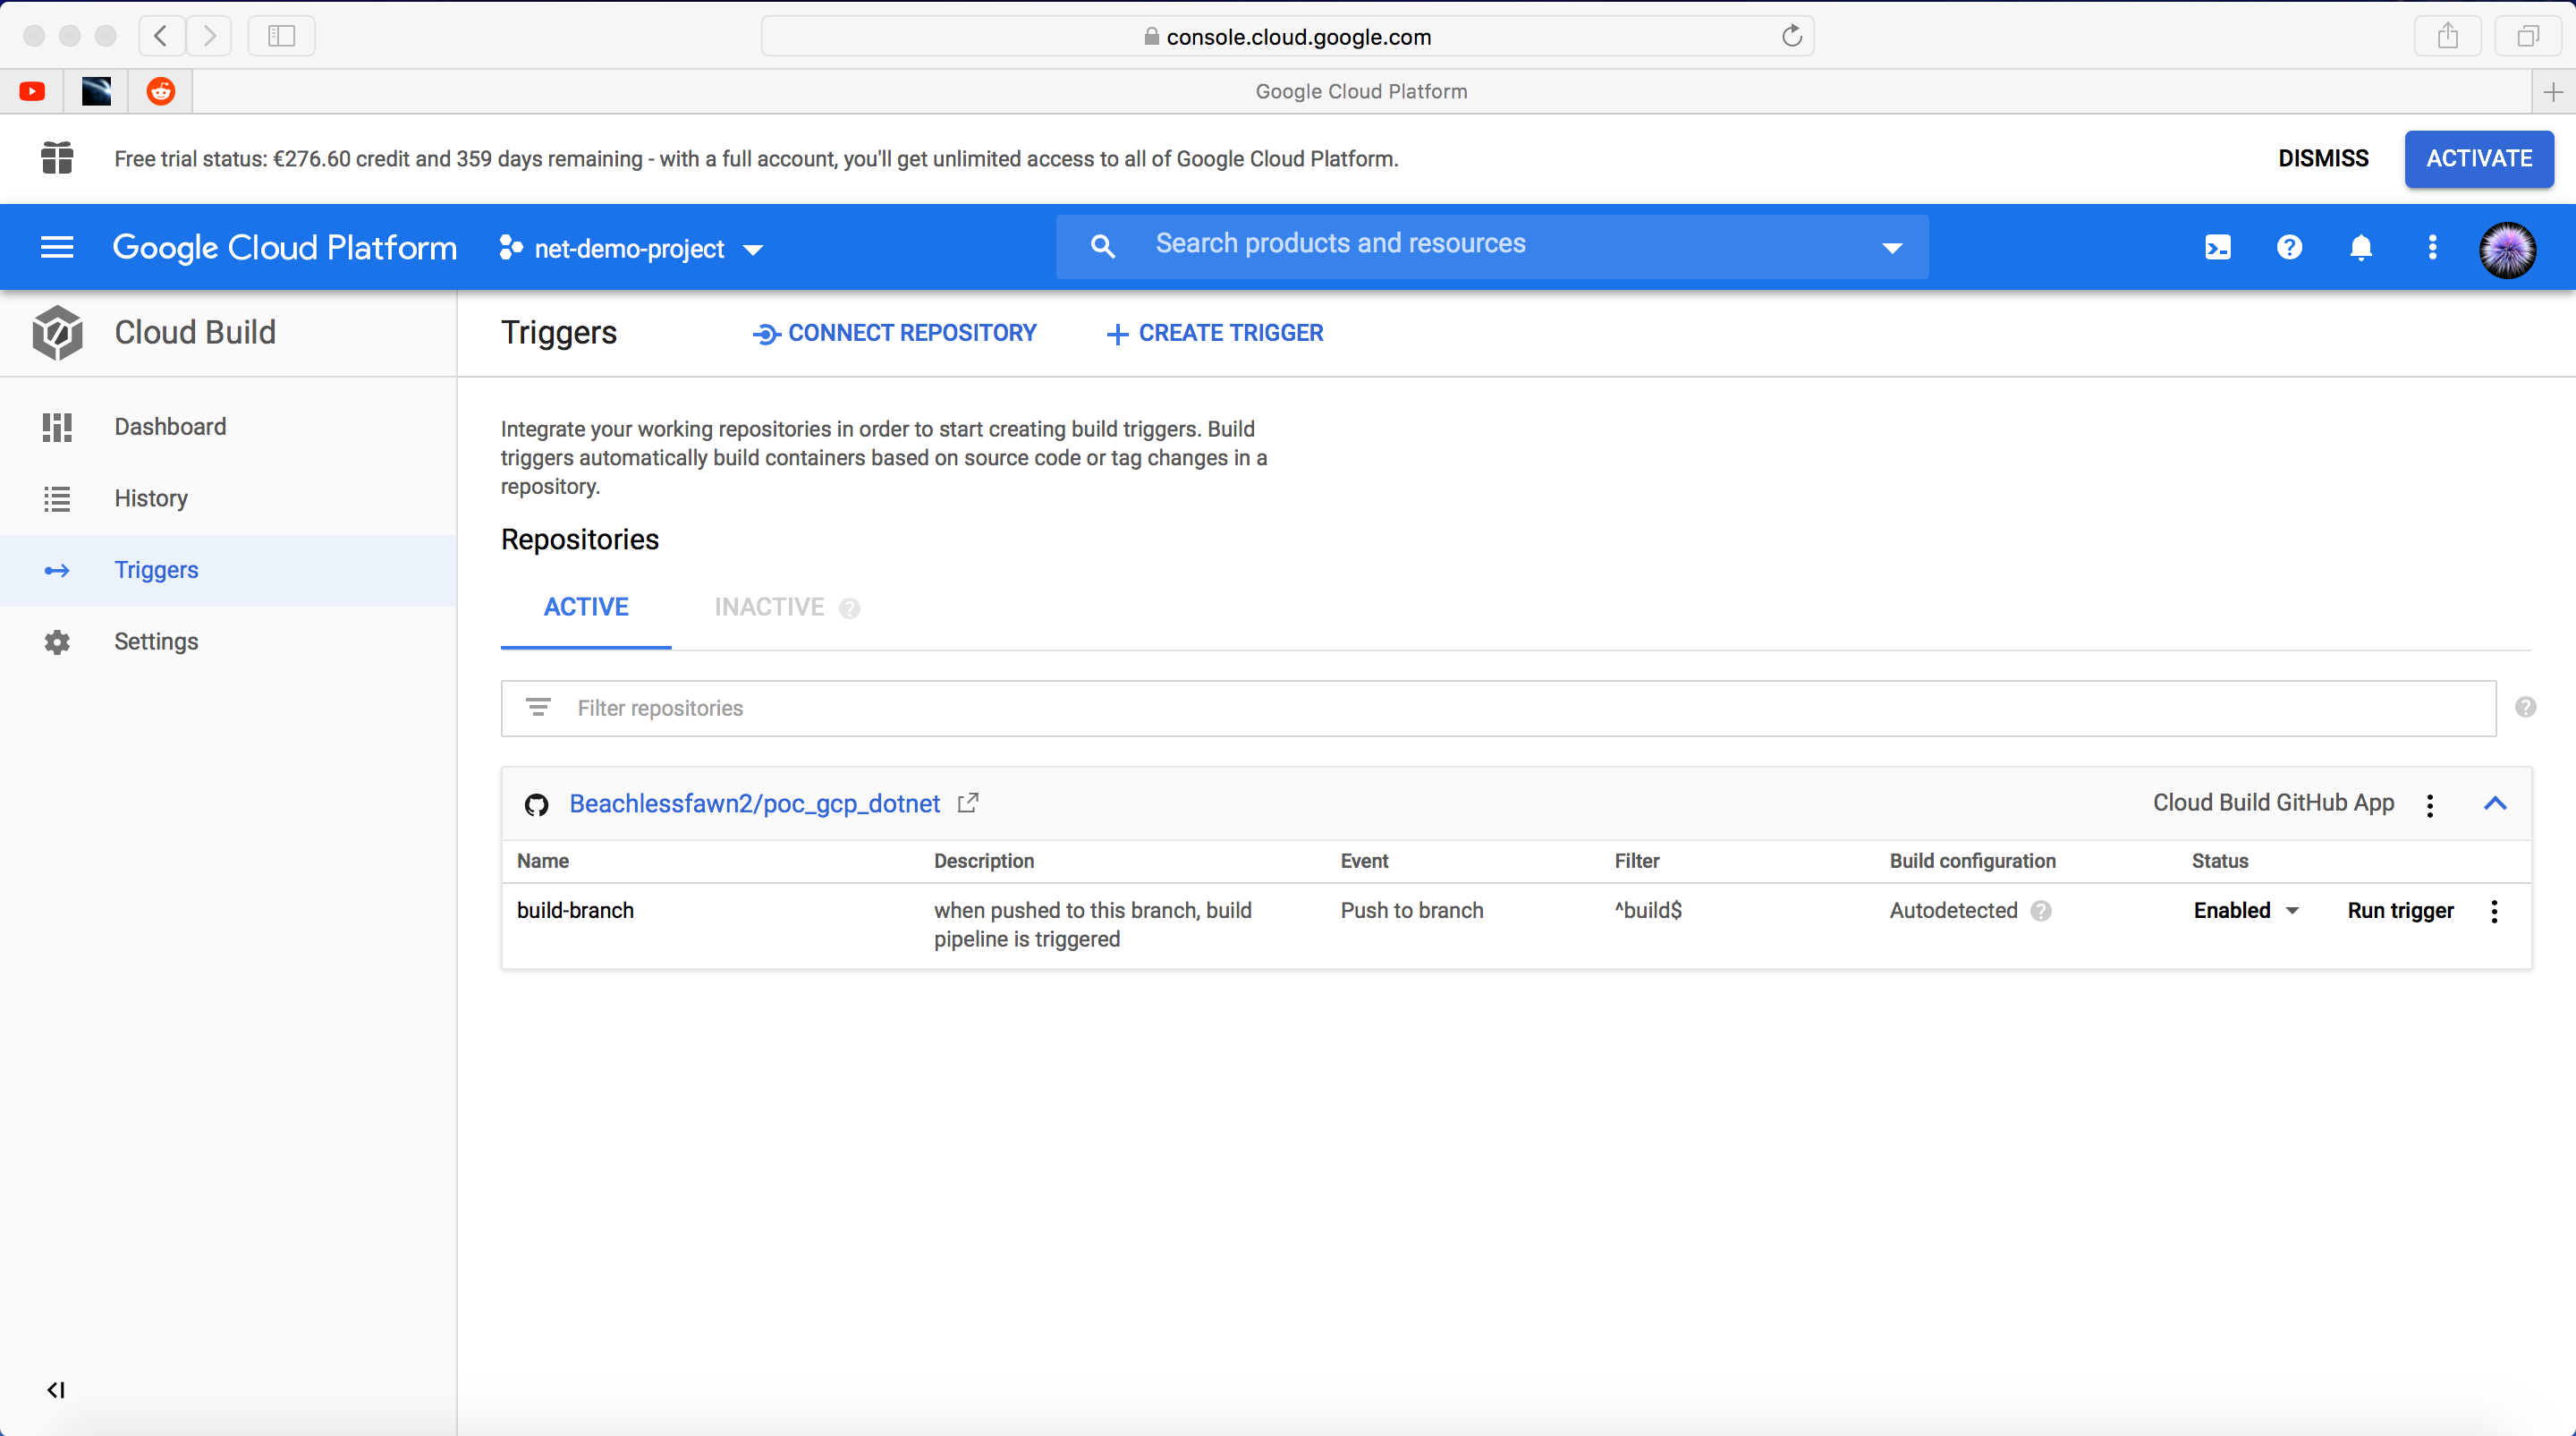
\includegraphics[width=\linewidth]{/Users/kenzie/Documents/HoGent/Bachelorproef/Images/gcp_net_demo_trigger.png}
    \caption{Figuur toont het scherm  van Google Cloud met een gecreëerde Trigger op de tak 'Build' op GitHub.}
    \label{fig:GCP_POC_trigger}
\end{figure}

Eenmaal dit gebeurd is kon de trigger getest worden door een commit uit te voeren op GitHub. Vervolgens was het resultaat te testen op de lokale Windows Server 2019. Ook was er een gedetailleerd rapport te zien op de console van Google Cloud zelf. Om de applicatie uit te voeren moest simpel weg het gecomprimeerde bestand uitgepakt worden en uitgevoerd worden. \emph{Figuur~\ref{fig:GCP_POC_result}} toont het resultaat van de uitgevoerde applicatie op de lokale machine. \emph{Figuur~\ref{fig:GCP_POC_run}} toont de uitgevoerde compilatie op Google Cloud.

\begin{figure}[!htbp]
    \centering
    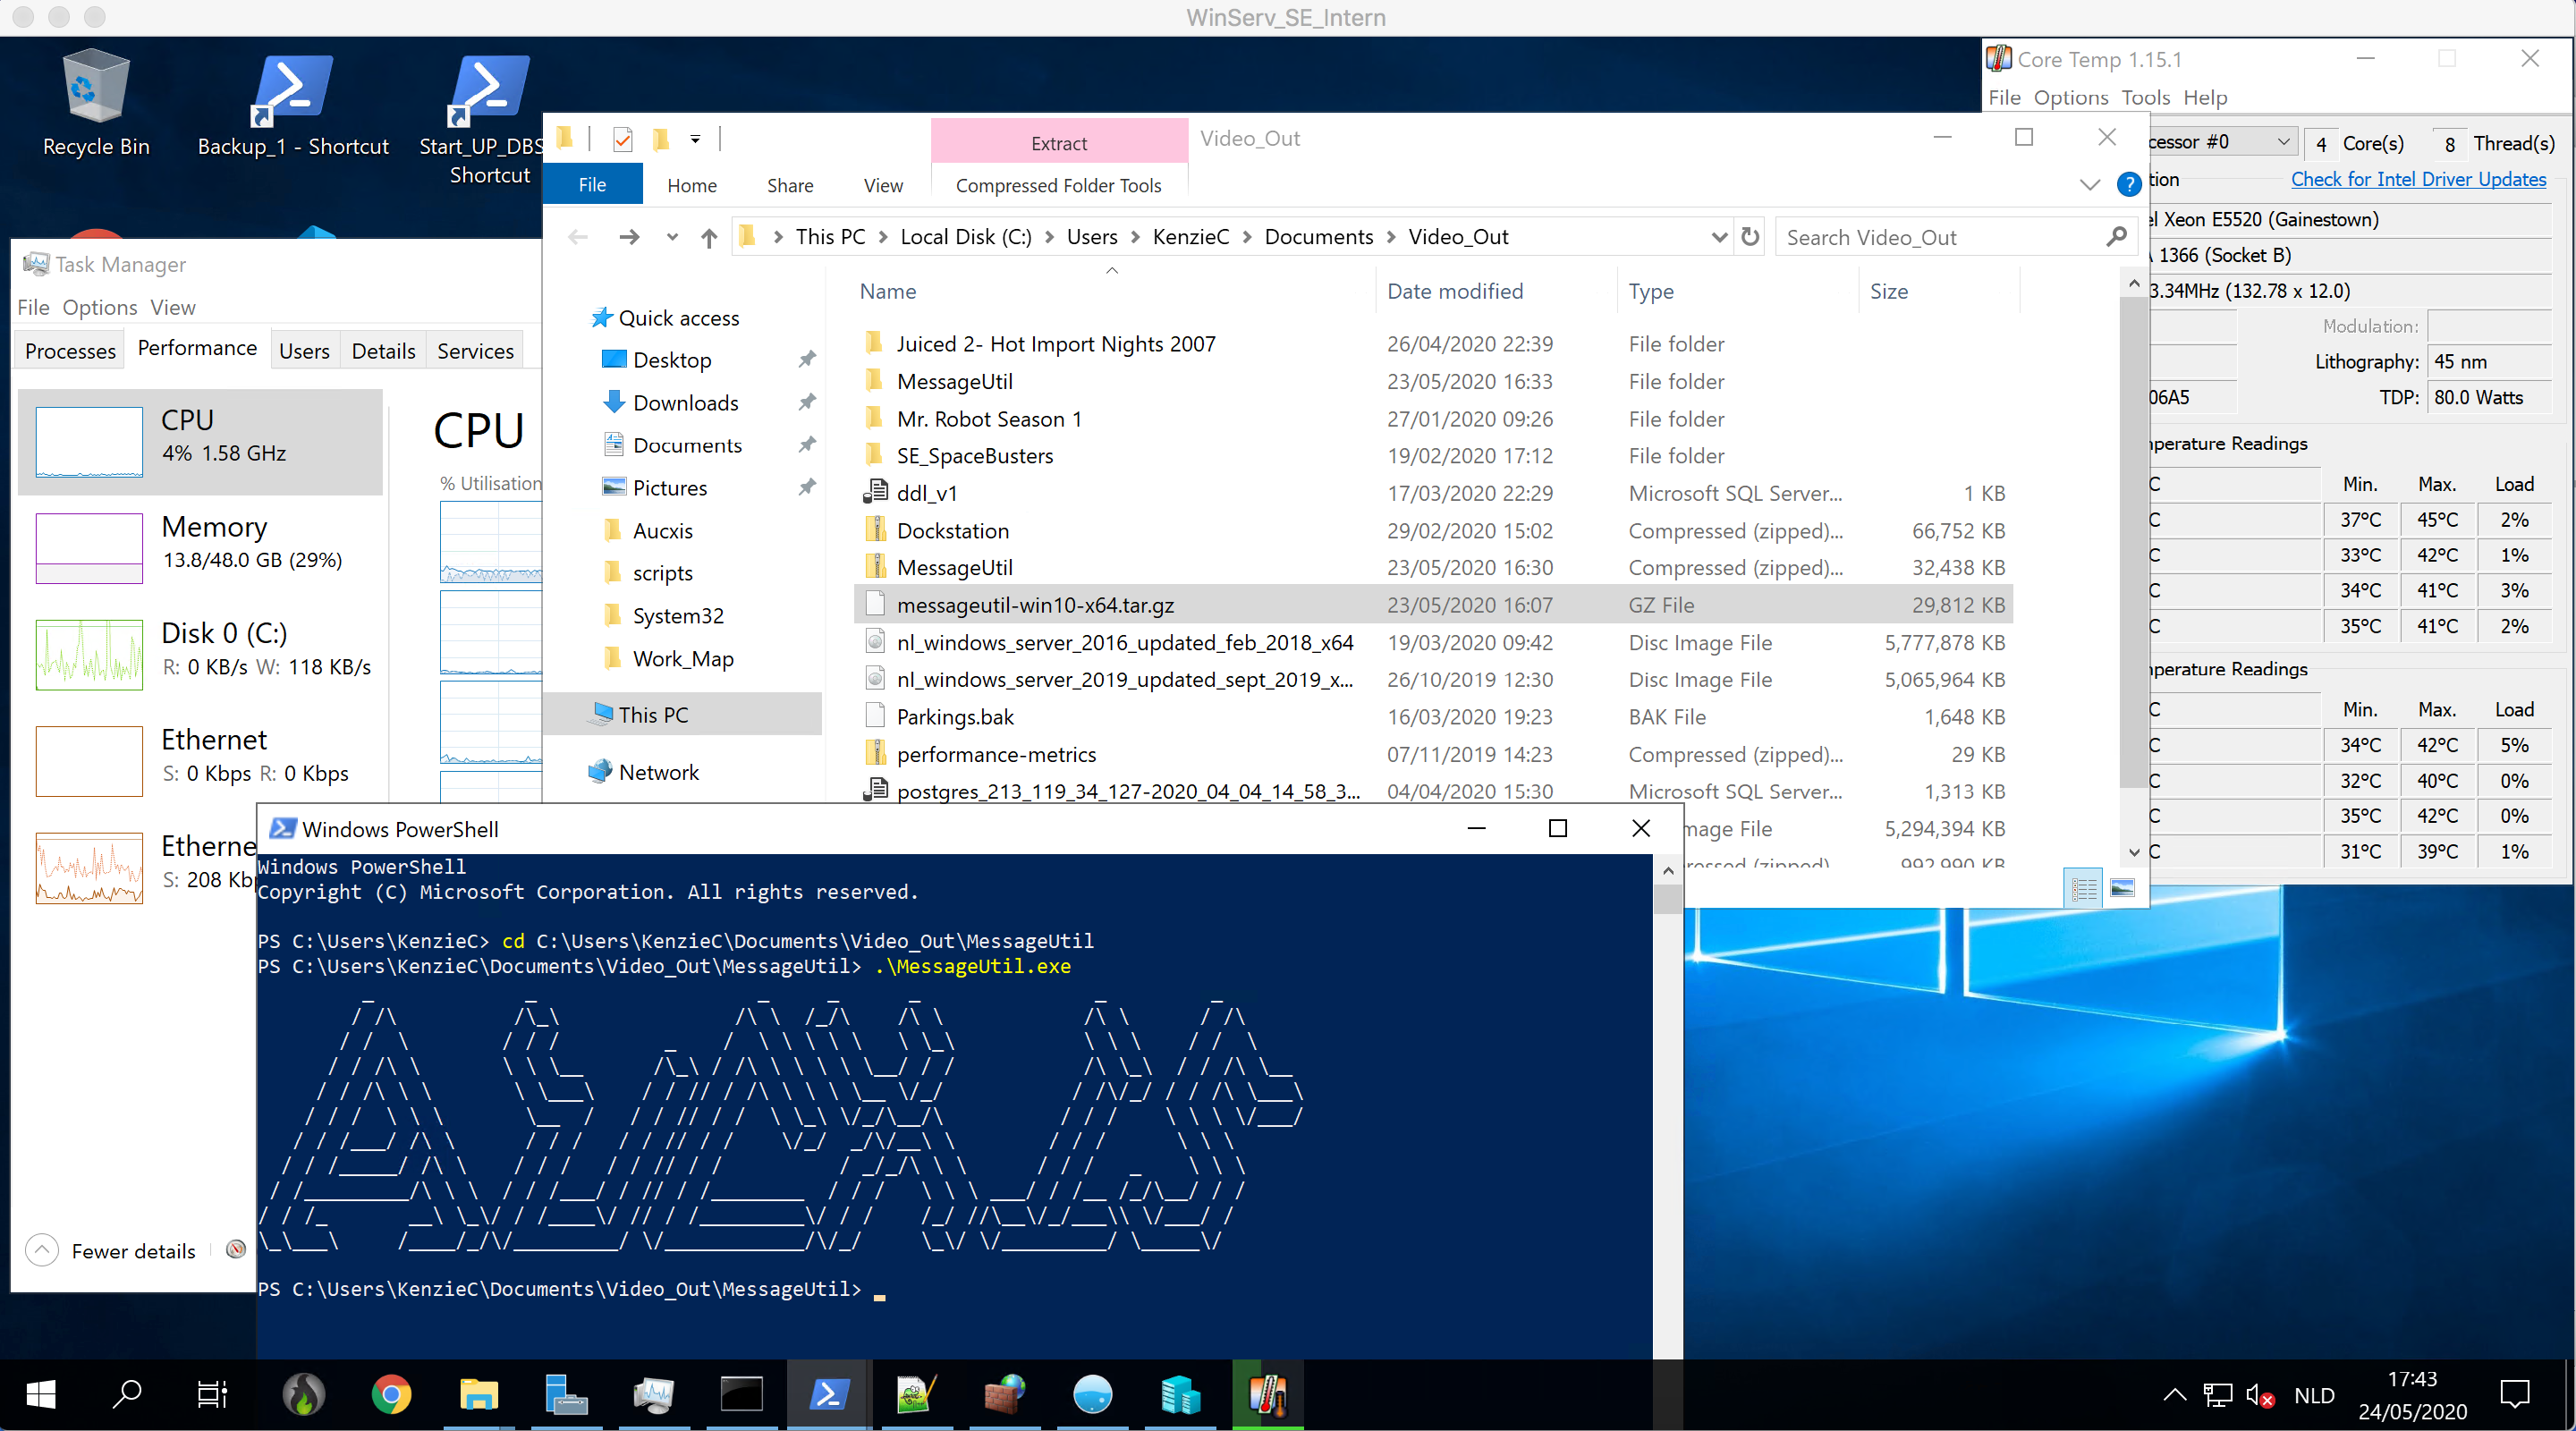
\includegraphics[width=\linewidth]{/Users/kenzie/Documents/HoGent/Bachelorproef/Images/gcp_net_demo_result.png}
    \caption{Figuur toont de uitvoer van de gecompileerde applicatie op een lokale Windows Server 2019. Applicatie is gekopieerd door middel van \emph{script~\ref{code:filetrans}}.}
    \label{fig:GCP_POC_result}
\end{figure}

\begin{figure}[!htbp]
    \centering
    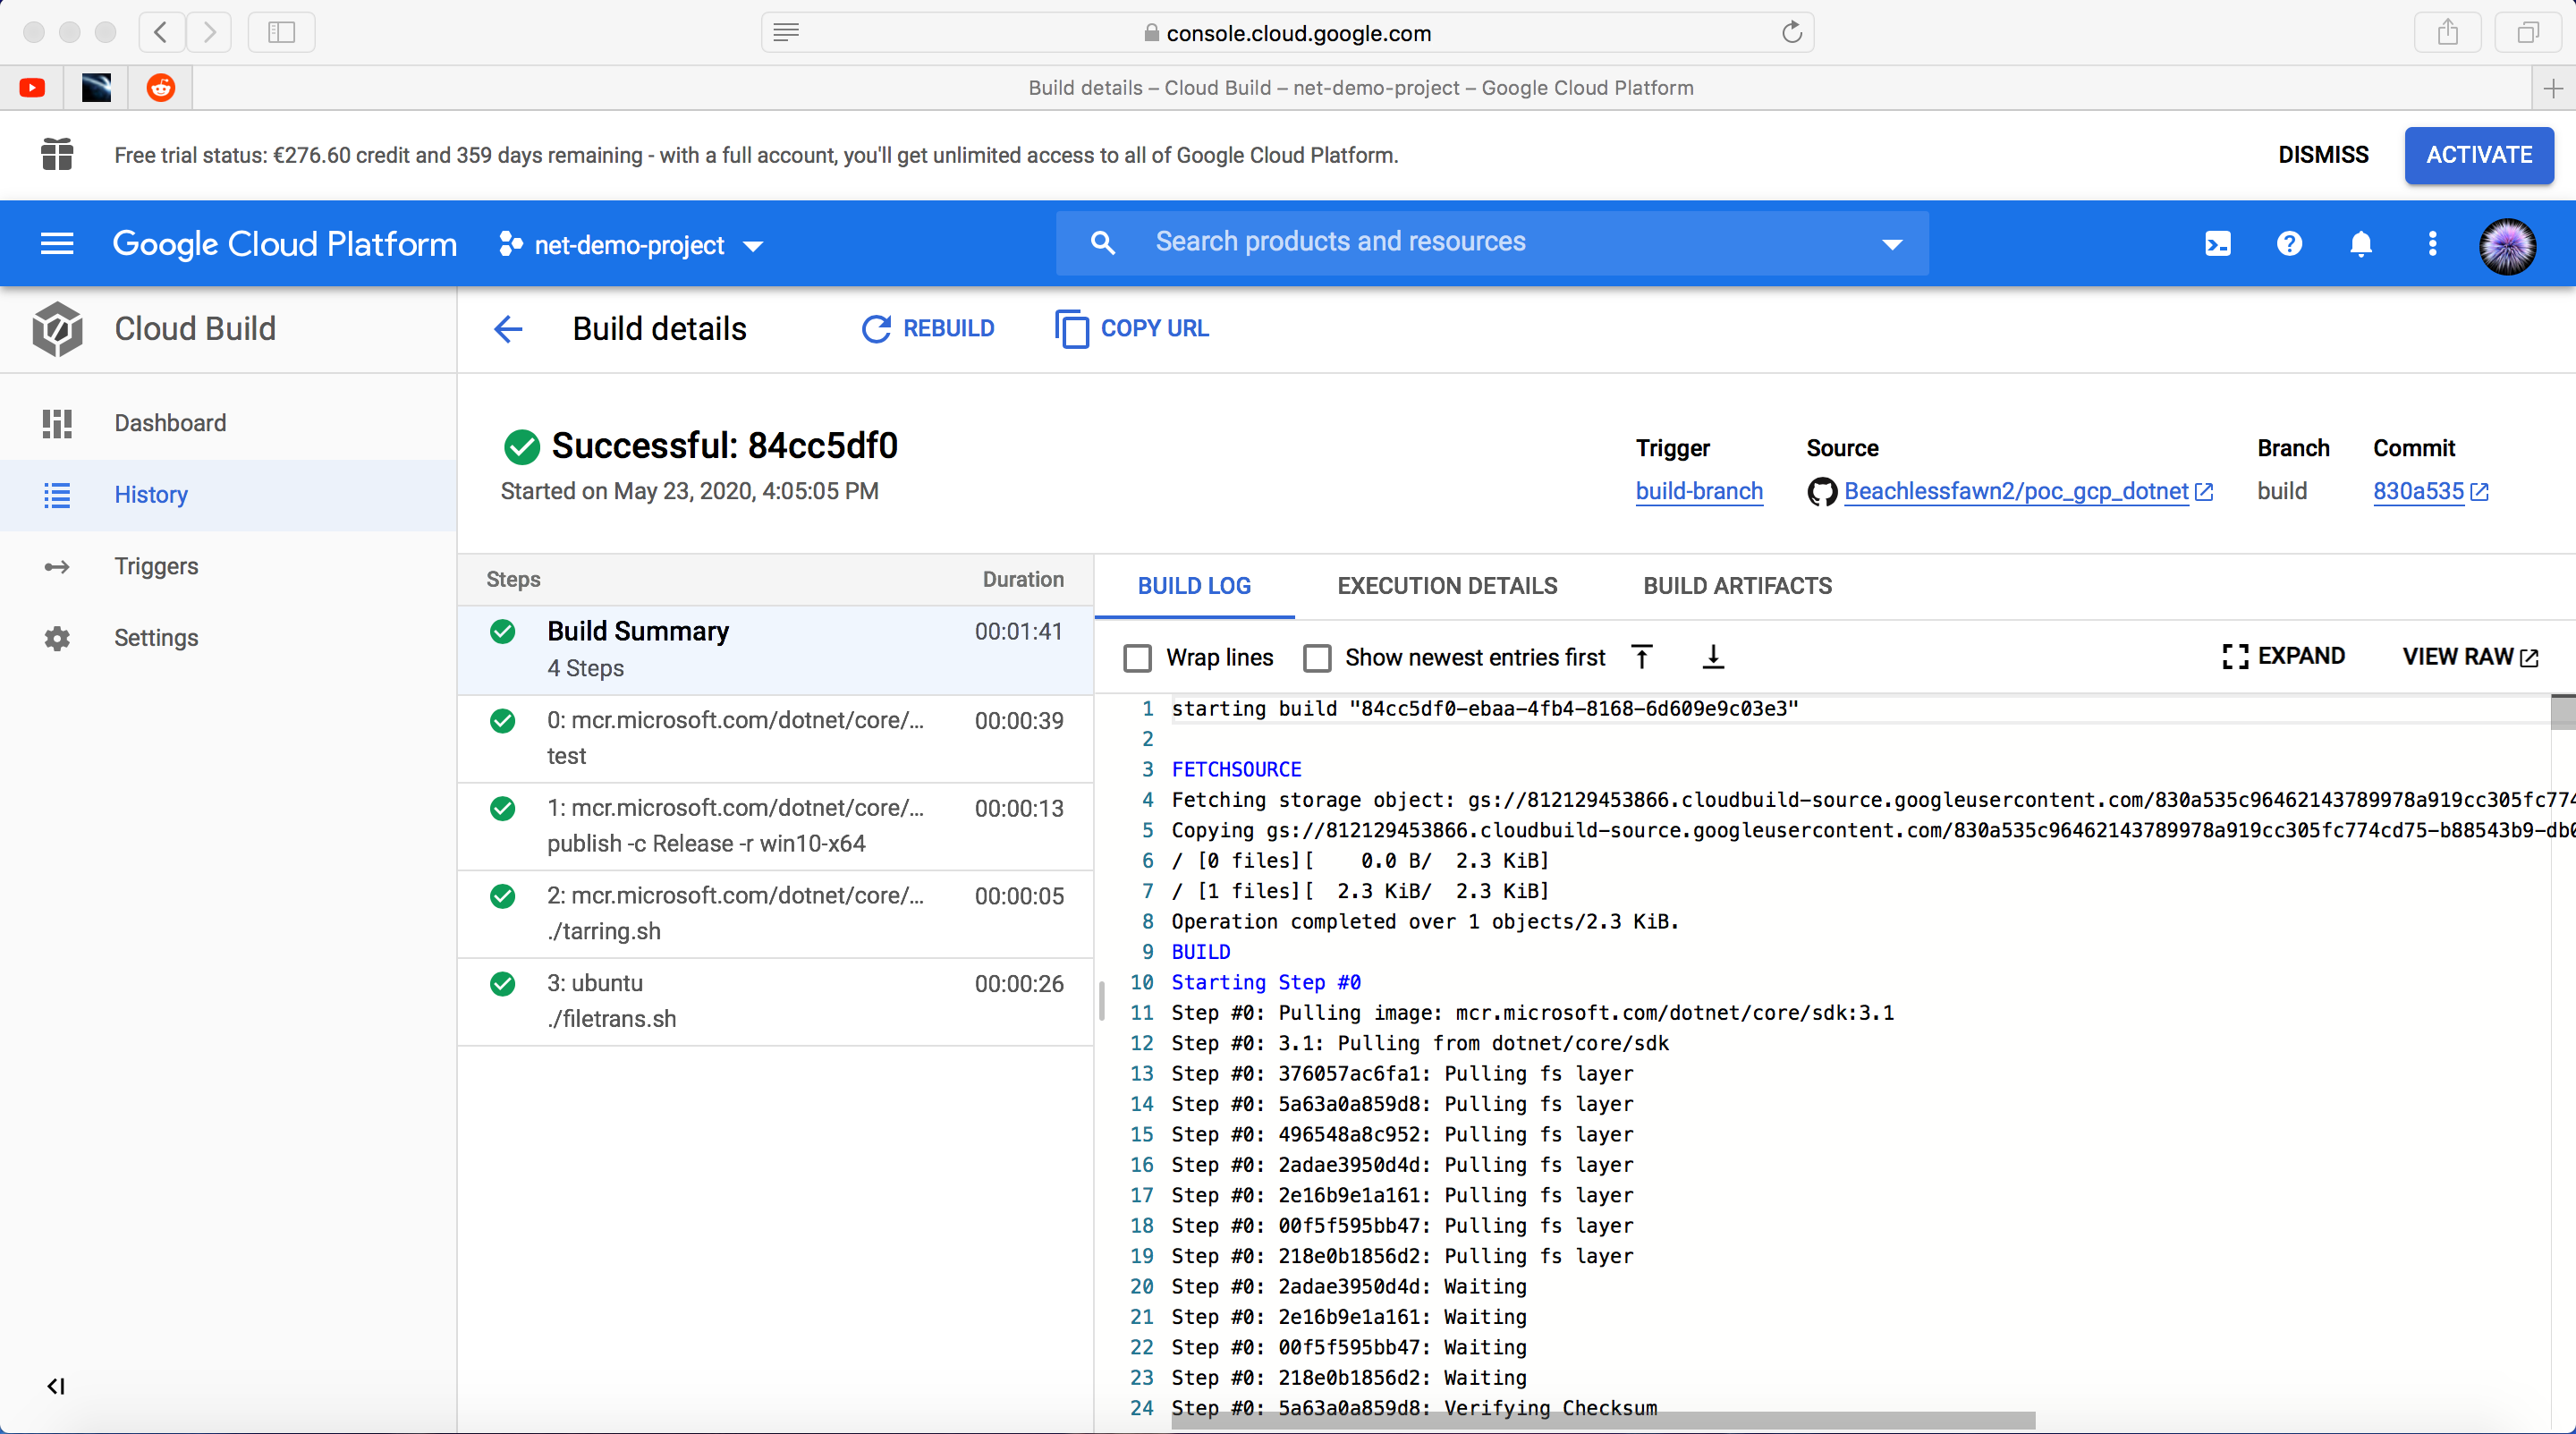
\includegraphics[width=\linewidth]{/Users/kenzie/Documents/HoGent/Bachelorproef/Images/gcp_net_demo_run.png}
    \caption{Figuur toont het resultaat van de compilatie stappen op Google Cloud. Ook zijn er een aantal andere logs te bekijken op dit scherm.}
    \label{fig:GCP_POC_run}
\end{figure}

Tot slot is er op de online console van Google Cloud een simpel dashboard te zien. Dit dashboard toont de laatst uitgevoerde compilatie trigger van het project. Ook toont het eventuele fouten, gemiddelde tijden, wat de compilatie heeft doen uitvoeren, commit ID van GitHub, enz. \emph{Figuur~\ref{fig:GCP_POC_dashboard}} toont een voorbeeld van zo een dashboard.

\begin{figure}[!htbp]
    \centering
    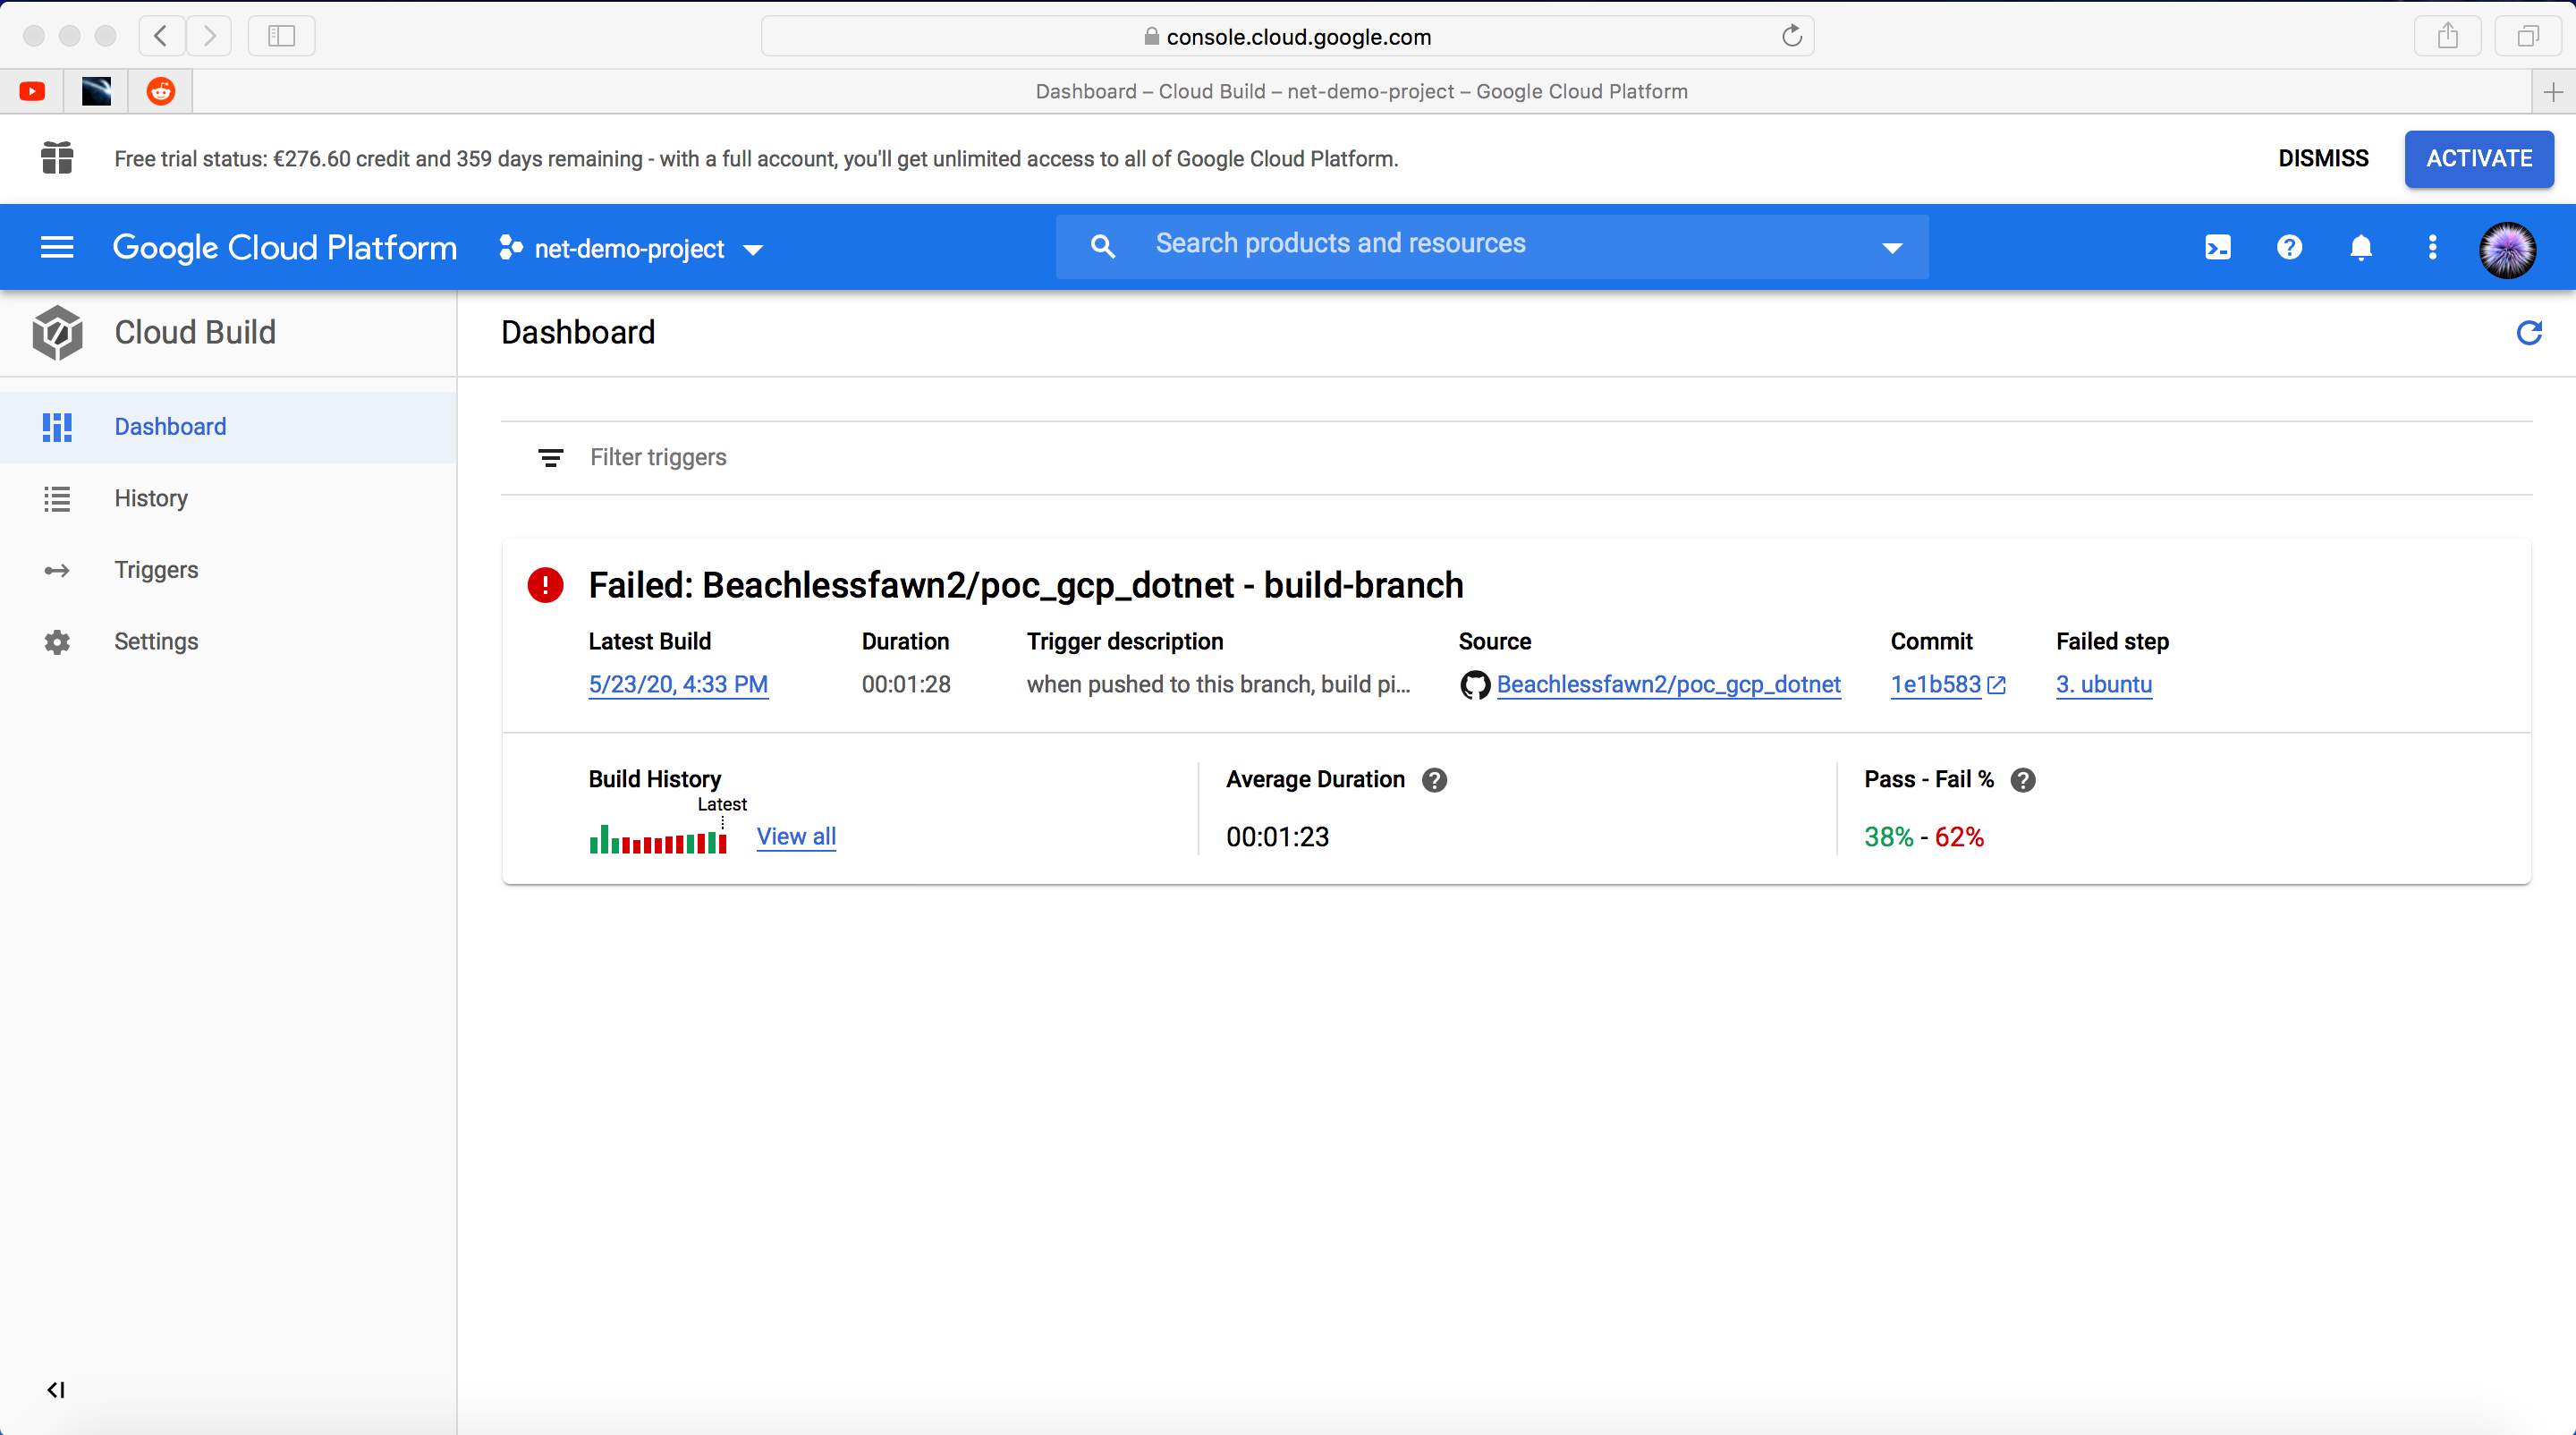
\includegraphics[width=\linewidth]{/Users/kenzie/Documents/HoGent/Bachelorproef/Images/gcp_net_demo_dashboard.png}
    \caption{Figuur toont een simpel dashboard met gegevens over de compilatie pijpleiding.}
    \label{fig:GCP_POC_dashboard}
\end{figure}

Door deze POC op te stellen is er gebleken dat Google Cloud Build Code gemakkelijk te gebruiken is. Dat is, eenmaal de gebruiker er thuis in is. Er bestaat redelijk wat documentatie over wat allemaal mogelijk is in een ‘cloudbuild.yaml’. Helaas is voor een beginner het niet gemakkelijk om te verstaan hoe de verschillende containers met elkaar samenwerken en waar nu alle bestanden staan. Ook is een goede kennis van de containers nodig om te kunnen verstaan wat er allemaal mogelijk is. Dit zorgt ervoor dat het lang kan duren vooraleer er een pijpleiding operationeel is. Ook is het spijtig dat er niet meer analytics te verkrijgen zijn op Google Cloud Code Build. De gebruiker heeft enkel de analytics van wat er door Google zelf wordt aangeboden. Na het opstellen van deze POC is er ook gebleken dat Google Cloud niet zo duur is. Al het testen en uitproberen heeft slechts 0.40 euro gekost.
 Het kan interessant zijn om in een later onderzoek te kijken of het niet mogelijk is om de gegenereerde log bestanden van Google Cloud te downloaden en te gebruiken voor eigen visualisatie systemen zoals: Grafana. 

\subsection{Azure DeVops}
\label{sec:VergelijkingADV}
Naast de POC op Google Cloud is het ook nog interessant om dezelfde opstelling eens te maken in Azure DeVops. Dit om de ervaring en de functionaliteit naast elkaar te kunnen leggen. Voor de POC op Azure DeVops is er een nieuw DeVops project aangemaakt. Dit project heeft de naam ‘poc\_azure\_dotnet’ gekregen. \emph{Figuur~\ref{fig:Azure_POC_proj}} toont het aangemaakte project. Net zoals GCP bevatten projecten alle toegewezen producten en services die geconfigureerd geweest zijn. Ook is het gemakkelijk opnieuw te verwijderen en stopt dan ook de aanrekening.

\begin{figure}[!htbp]
    \centering
    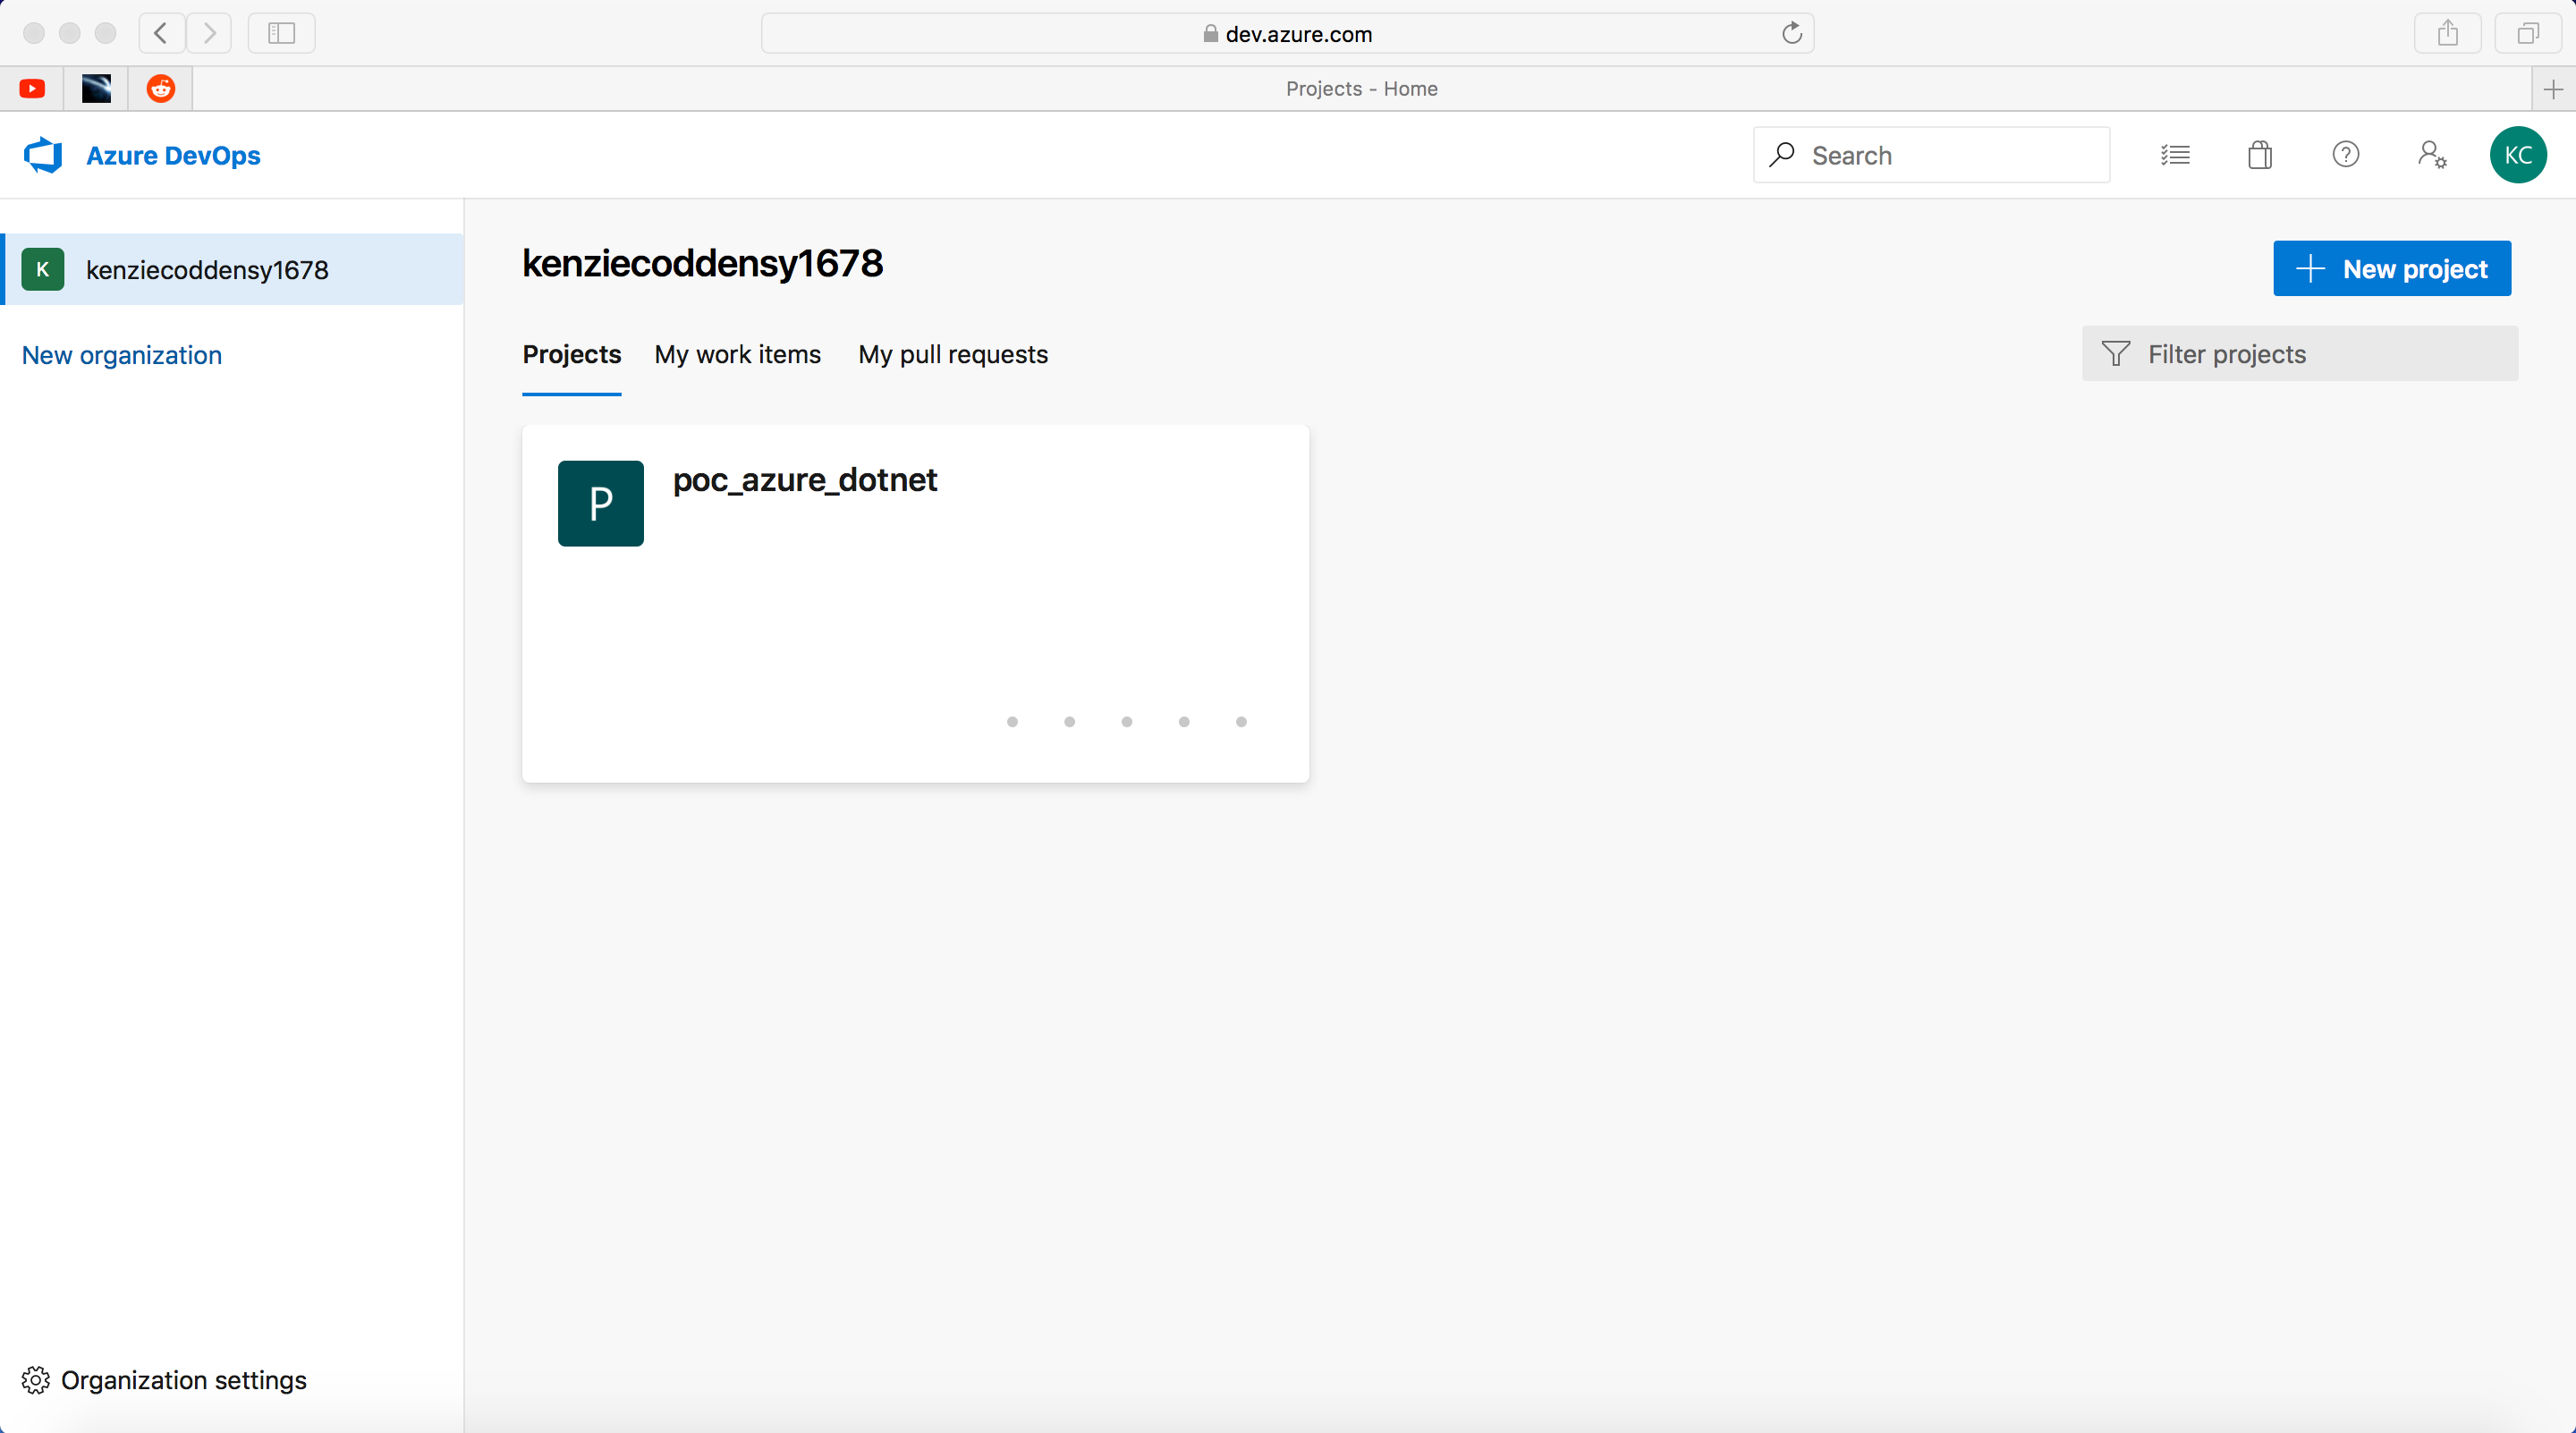
\includegraphics[width=\linewidth]{/Users/kenzie/Documents/HoGent/Bachelorproef/Images/azure_net_demo_proj.png}
    \caption{Figuur toont een nieuw aangemaakt project op Azure DeVops.}
    \label{fig:Azure_POC_proj}
\end{figure}

Deze POC vertrekt vanuit dezelfde applicatie als bij GCP. Hiervoor is er een nieuwe map aangemaakt op de gebruiker zijn computer voor de applicatie. Deze is geïnitialiseerd als een Git repositorie. Hierin zijn dan de bestanden \emph{MessageUtil~\ref{code:messageutil}} \& \emph{MessageUtilTest~\ref{code:messageutiltest}} voor de .Net applicatie in geplaatst. Ook is er een gitignore aangemaakt. \emph{Figuur~\ref{code:azuregittree}} toont een tree van de bestanden en mappen structuur. Deze repositorie is dan geüpload naar GitHub.

\lstset{
    language=bash,
    caption={Tree van de bestanden structuur voor de Proof Of Concept op Azure DeVops.},
    label=code:azuregittree
}
\begin{lstlisting}
poc_azure_dotnet/
`--- .gitignore
`--- MessageUtil
    `--- MessageUtil.csproj
    `--- MessageUtilProgram.cs
`--- MessageUtil.sln
`--- MessageUtilTest
    `--- MessageUtilTest.csproj
    `--- MessageUtilTests.cs
\end{lstlisting}

Hierna is er op Azure DeVops een nieuwe pijpleiding aangemaakt. Dit was zeer gemakkelijk te volgen door middel van de online wizard. Eerst moest er gekozen worden wat versiebeheersysteem de gebruiker gebruikt. Hier is er gekozen voor GitHub. Vervolgens vraagt Azure DeVops de gebruiker toestemming voor het uitlezen van de repositories. Tegelijk wordt ook de Azure DeVops pijpleiding applicatie toegevoegd aan de gebruiker zijn GitHub. Na de initialisatie van de Azure DeVops applicatie voor GitHub moest er een reposirotrie geselecteerd worden. Hier is er gekozen voor de zojuist gemaakte GitHub repositorie. Azure DeVops leest deze repositorie uit en stelt dan op basis van de bestanden de juiste compilatie oplossing voor. Voor deze POC stelde Azure DeVops .Net Core voor als compilatie programma. Er is voor dezen oplossing gekozen. Azure DeVops toont hierna een Yaml-bestand, ‘azure-pipelines.yml’, met voor gemaakte stappen. Dit YAML-bestand bevat drie stappen. Een eerste stap die de juiste pakketten installeert op de virtuele machine. In een tweede stap wordt de applicatie gecompileerd. In de derde stap worden de meegeleverde testen uit \emph{MessagUtilTest~\ref{code:messageutiltest}} uitgevoerd. \emph{Figuur~\ref{code:azure-pipelines-poc}} toont dit YAML-bestand.

\lstset{
    language=bash,
    caption={YAML-bestand voor de configuratie van de .Net pijpleiding op Azure DeVops.},
    label=code:azure-pipelines-poc
}
\begin{lstlisting}
# .NET Desktop
# Build and run tests for .NET Desktop or Windows classic desktop solutions.
# Add steps that publish symbols, save build artifacts, and more:
# https://docs.microsoft.com/azure/devops/pipelines/apps/windows/dot-net

trigger:
    - master

pool:
    vmImage: 'windows-latest'

variables:
    solution: '**/*.sln'
    buildPlatform: 'Any CPU'
    buildConfiguration: 'Release'

steps:
- task: NuGetToolInstaller@1

- task: NuGetCommand@2
    inputs:
    restoreSolution: '$(solution)'

- task: VSBuild@1
    inputs:
    solution: '$(solution)'
    platform: '$(buildPlatform)'
    configuration: '$(buildConfiguration)'

- task: VSTest@2
    inputs:
    platform: '$(buildPlatform)'
    configuration: '$(buildConfiguration)'
\end{lstlisting}

Verwacht was dat dit een werkend vertrekpunt is voor de pijpleiding. Zeker omdat deze applicatie met een Microsoft specifieke taal gemaakt is, met behulp van het .Net framework dat ook Microsoft specifiek is. In eerste instantie leek deze pijpleiding te werken. Maar na het bekijken van de logbestanden is er vastgesteld dat de testen niet werden uitgevoerd. Er is gezocht naar een oplossing voor dit probleem. Er is geen duidelijke oplossing gevonden voor de huidige configuratie. De documentatie over deze modules was zeer onduidelijk en moeilijk te begrijpen. Zeker vanuit het standpunt van een beginner. In dit opzicht is er gekozen om opnieuw te beginnen aan de hand van een andere \emph{\href{https://docs.microsoft.com/en-us/azure/devops/pipelines/ecosystems/dotnet-core?view=azure-devops}{handleiding}} op Azure. Deze gebruikt een voor gemaakte Windows virtuele machine met .Net core voor geïnstalleerd. Over deze module is uitgebreide documentatie te vinden. Daarnaast zijn er door Microsoft ook voorbeelden ter beschikking. Dit was dan ook het perfecte vertrekpunt.

Dit nieuw YAML-bestand bestaat uit zes stappen. In een eerste stap wordt de ‘MessageUtil’ applicatie volledige herbouwt. Deze staat dan klaar voor verdere stappen. In de tweede stap wordt de applicatie gecompileerd. De derde stap voert de meegeleverde testen uit. Ook publiceert het de resultaten op Azure DeVops. \emph{Figuur~\ref{fig:Azure_POC_testr}} toont een voorbeeld van uitgevoerde testen. De vierde stap compileert een uitrol versie voor het 64 bit Windows 10 platform in een map, publish. In de vijfde stap wordt er een PowerShell script uitgevoerd. Dit Script comprimeert de map publish. \emph{Figuur~\ref{code:zipping}} toont het ‘zipping.ps1’ script. In een laatste stap wordt deze gecomprimeerde map gepubliceerd als een artifact zodanig dat de applicatie klaarstaat om in een latere stap te worden uitgerold. \emph{Figuur~\ref{code:azure-pipelines-poc-n}} toont het verbeterde ‘azure-pipelines.yml’. Vervolgens is deze code toegevoegd op GitHub.

\begin{figure}[!htbp]
    \centering
    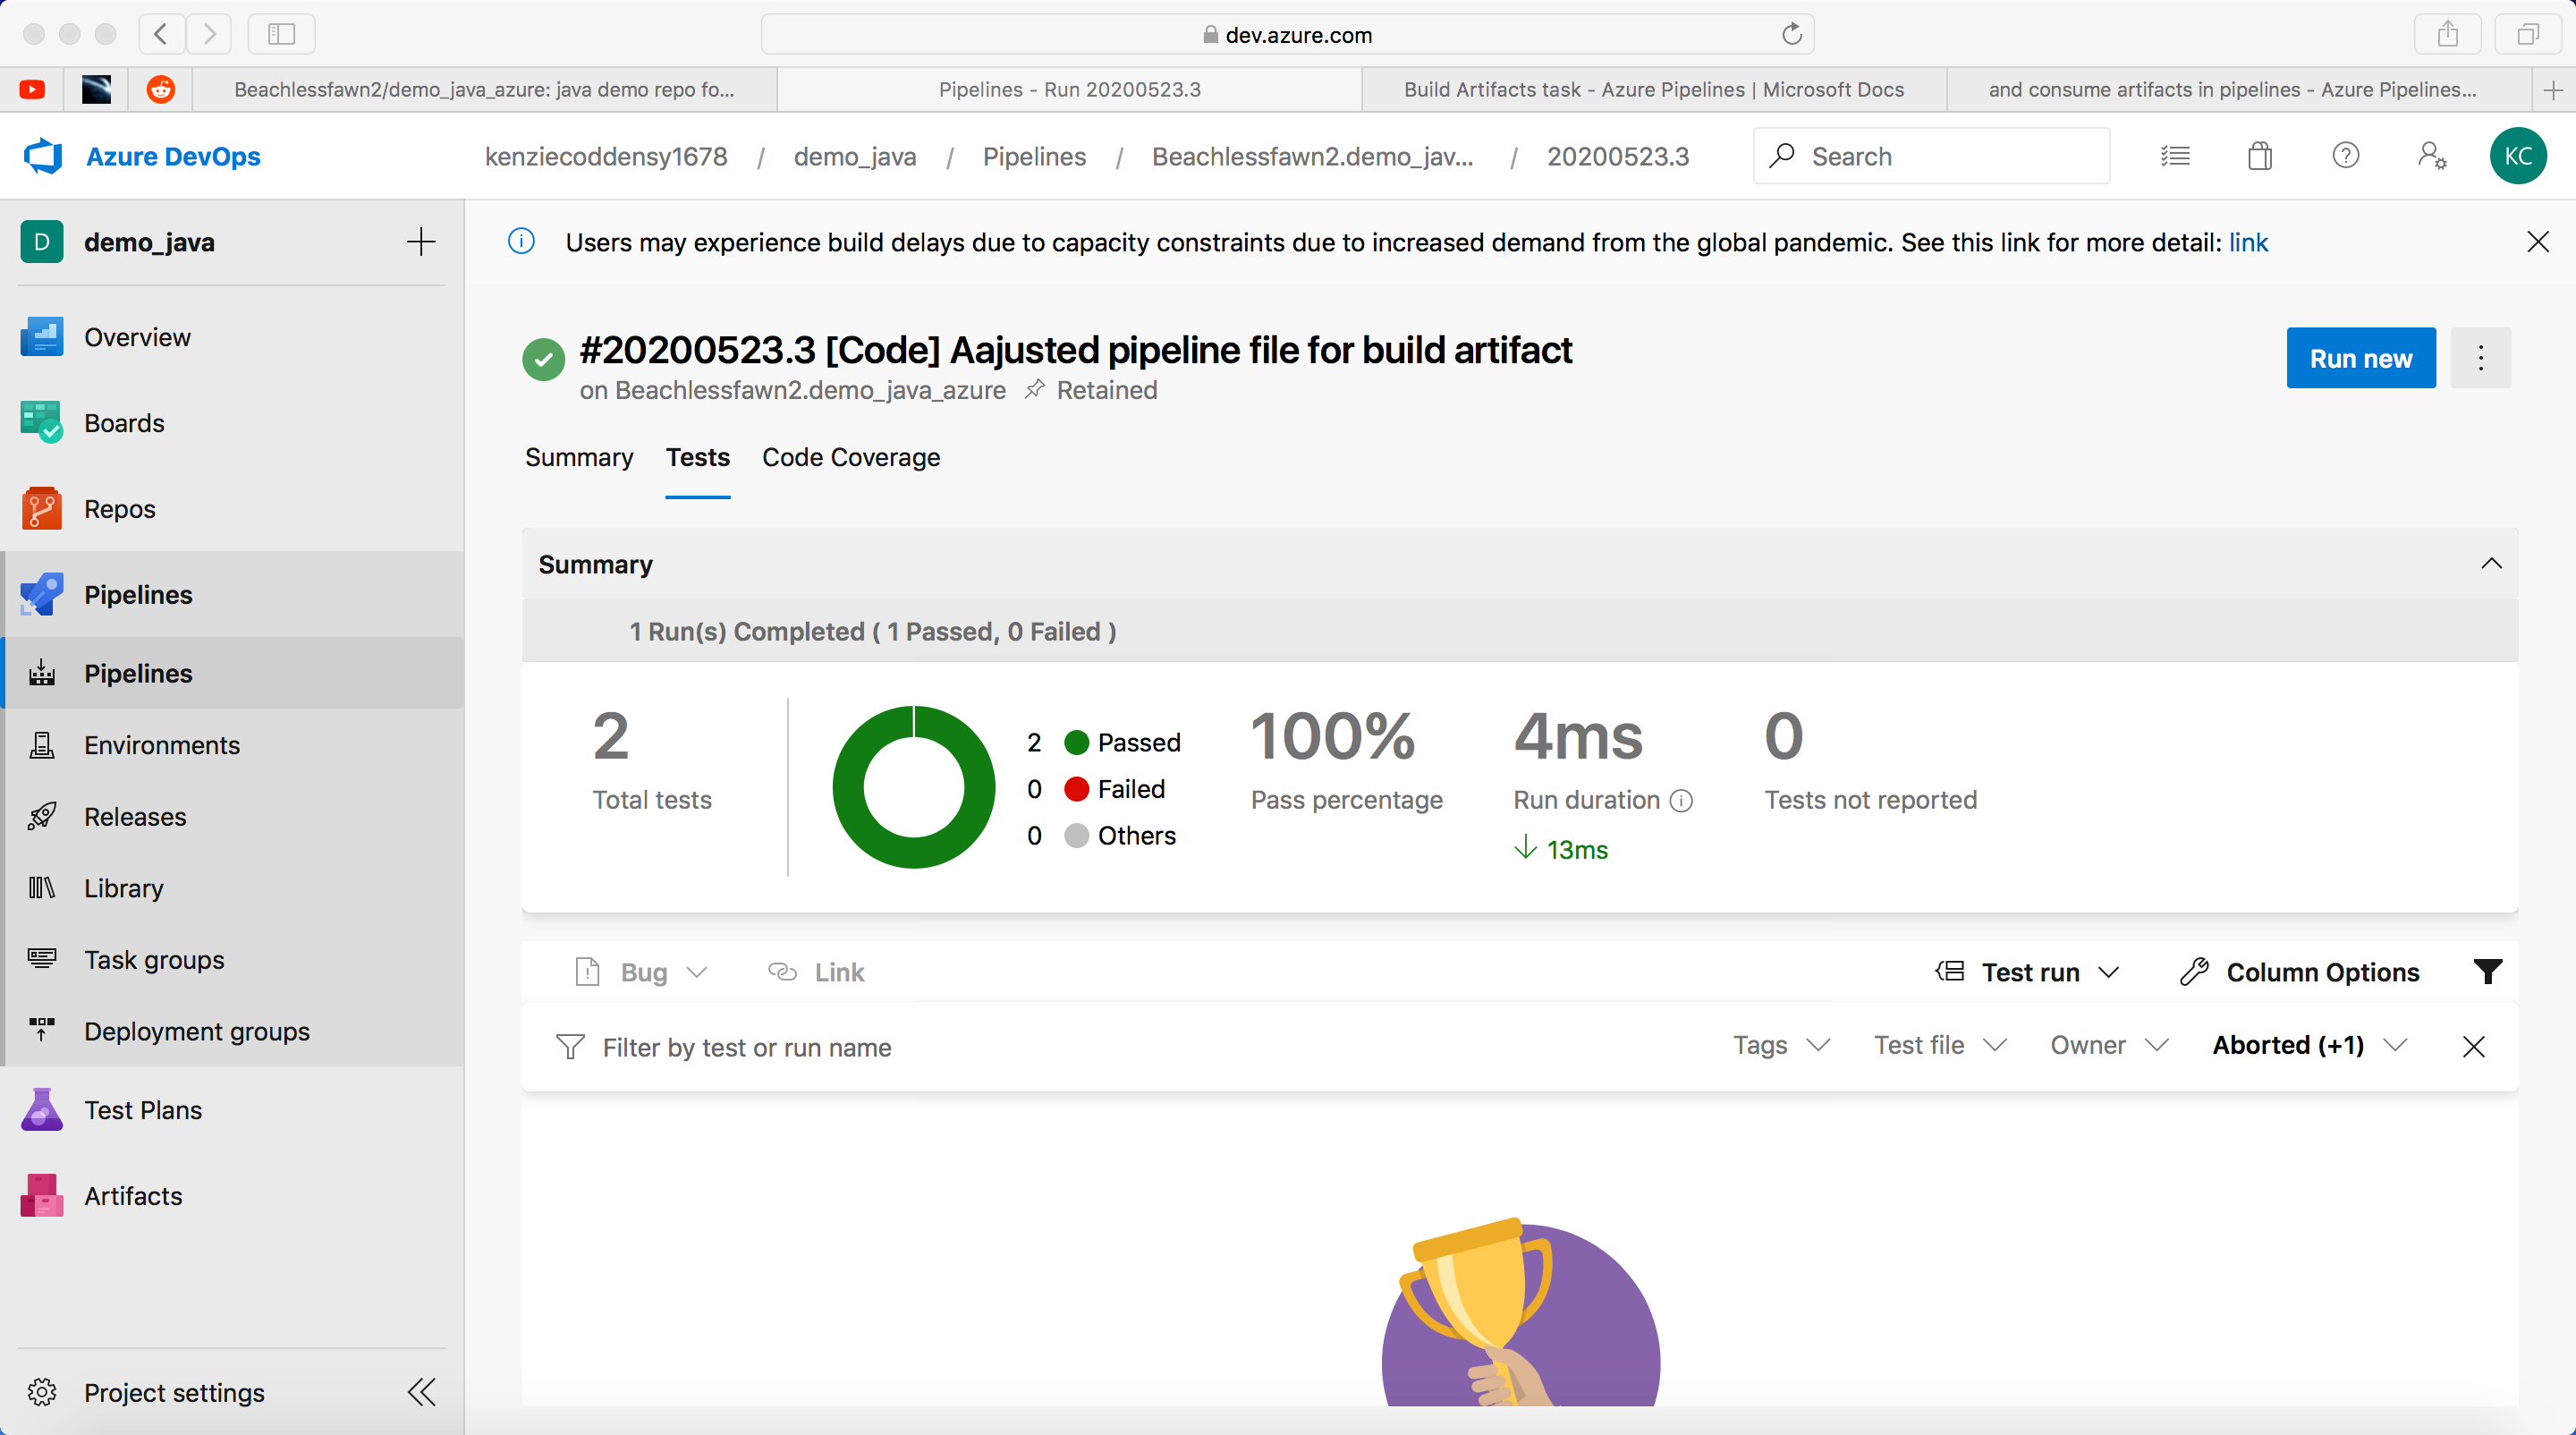
\includegraphics[width=\linewidth]{/Users/kenzie/Documents/HoGent/Bachelorproef/Images/azure_net_demo_testr.png}
    \caption{Figuur toont een simpel dashboard met gegevens over de uitgevoerde testen.}
    \label{fig:Azure_POC_testr}
\end{figure}

\lstset{
    language=C,
    caption={PowerShell script dat een map compresseert. Wordt gebruikt om alle .Net Framework afhankelijkheden mee te verpakken.},
    label=code:zipping
}
\begin{lstlisting}
$compress = @{
Path= "d:\a\1\s\MessageUtil\bin\Release\netcoreapp3.1\win10-x64\publish\*"
CompressionLevel = "Fastest"
DestinationPath = "d:\a\1\s\MessageUtil.zip"
}
Compress-Archive @compress
\end{lstlisting}

\lstset{
    language=bash,
    caption={Verbeterd YAML-bestand voor de configuratie van de .Net pijpleiding op Azure DeVops.},
    label=code:azure-pipelines-poc-n
}
\begin{lstlisting}
trigger:
    - master

pool:
    vmImage: 'windows-latest'

variables:
    buildConfiguration: 'Release'
    runtimeIdentifier: 'win10-x64'

steps:
- task: DotNetCoreCLI@2
    inputs:
        command: 'restore'
        restoreDirectory: '$(System.DefaultWorkingDirectory)'
        #packDirectory: '$(System.DefaultWorkingDirectory)'
        displayName: 'DotNet Restore Project'

- task: DotNetCoreCLI@2
    inputs:
        command: 'build'
        arguments: '--configuration $(buildConfiguration)'
        displayName: 'DotNet Build $(buildConfiguration)'

- task: DotNetCoreCLI@2
    inputs:
        command: 'test'
        projects: '**/*Test/*.csproj'
        arguments: '--configuration $(buildConfiguration) --collect "Code coverage"'
        displayName: 'DotNet Test Build'
    
- task: DotNetCoreCLI@2
    inputs:
        command: 'publish'
        publishWebProjects: false
        arguments: '--configuration $(buildConfiguration) -r $(runtimeIdentifier)'
        zipAfterPublish: false
        displayName: 'DotNet Publish Build'

- task: PowerShell@2
    inputs:
        targetType: 'filePath'
        filePath: $(System.DefaultWorkingDirectory)\ziping.ps1
        errorActionPreference: 'stop'
        displayName: 'DotNet Zip Publish'

- task: PublishPipelineArtifact@1
    inputs:
        targetPath: $(System.DefaultWorkingDirectory)\MessageUtil.zip
        artifactName: MessageUtil
        displayName: 'Upload Zip'
\end{lstlisting}

Het CI-gedeelte van de pijpleiding werkt met deze code. Voor het CD-gedeelte moest er een nieuwe uitrol pijpleiding gemaakt worden. Op Azure DeVops is er een nieuwe release gemaakt bestaande uit een Linux Ubuntu machine. Deze virtuele machine download het gemaakte artifact en verzend dit bestand naar de lokale Windows Server. Deze virtuele machine voert het script uit \emph{figuur~\ref{code:filetrans}} uit. Het instellen van deze uitrol pijpleiding is zeer gemakkelijk door de online wizard. \emph{Figuur~\ref{fig:Azure_POC_release}} toont het instellen van de virtuele machine. Ook zijn er talloze opties voor het instellen van toestemmingen, rechten, controles, enz. Dit kan interessant zijn in een productie omgeving. Deze POC laat dit buiten beschouwing. \emph{Figuur~\ref{fig:Azure_POC_pijp}} toont de volledige pijpleiding.

\begin{figure}[!htbp]
    \centering
    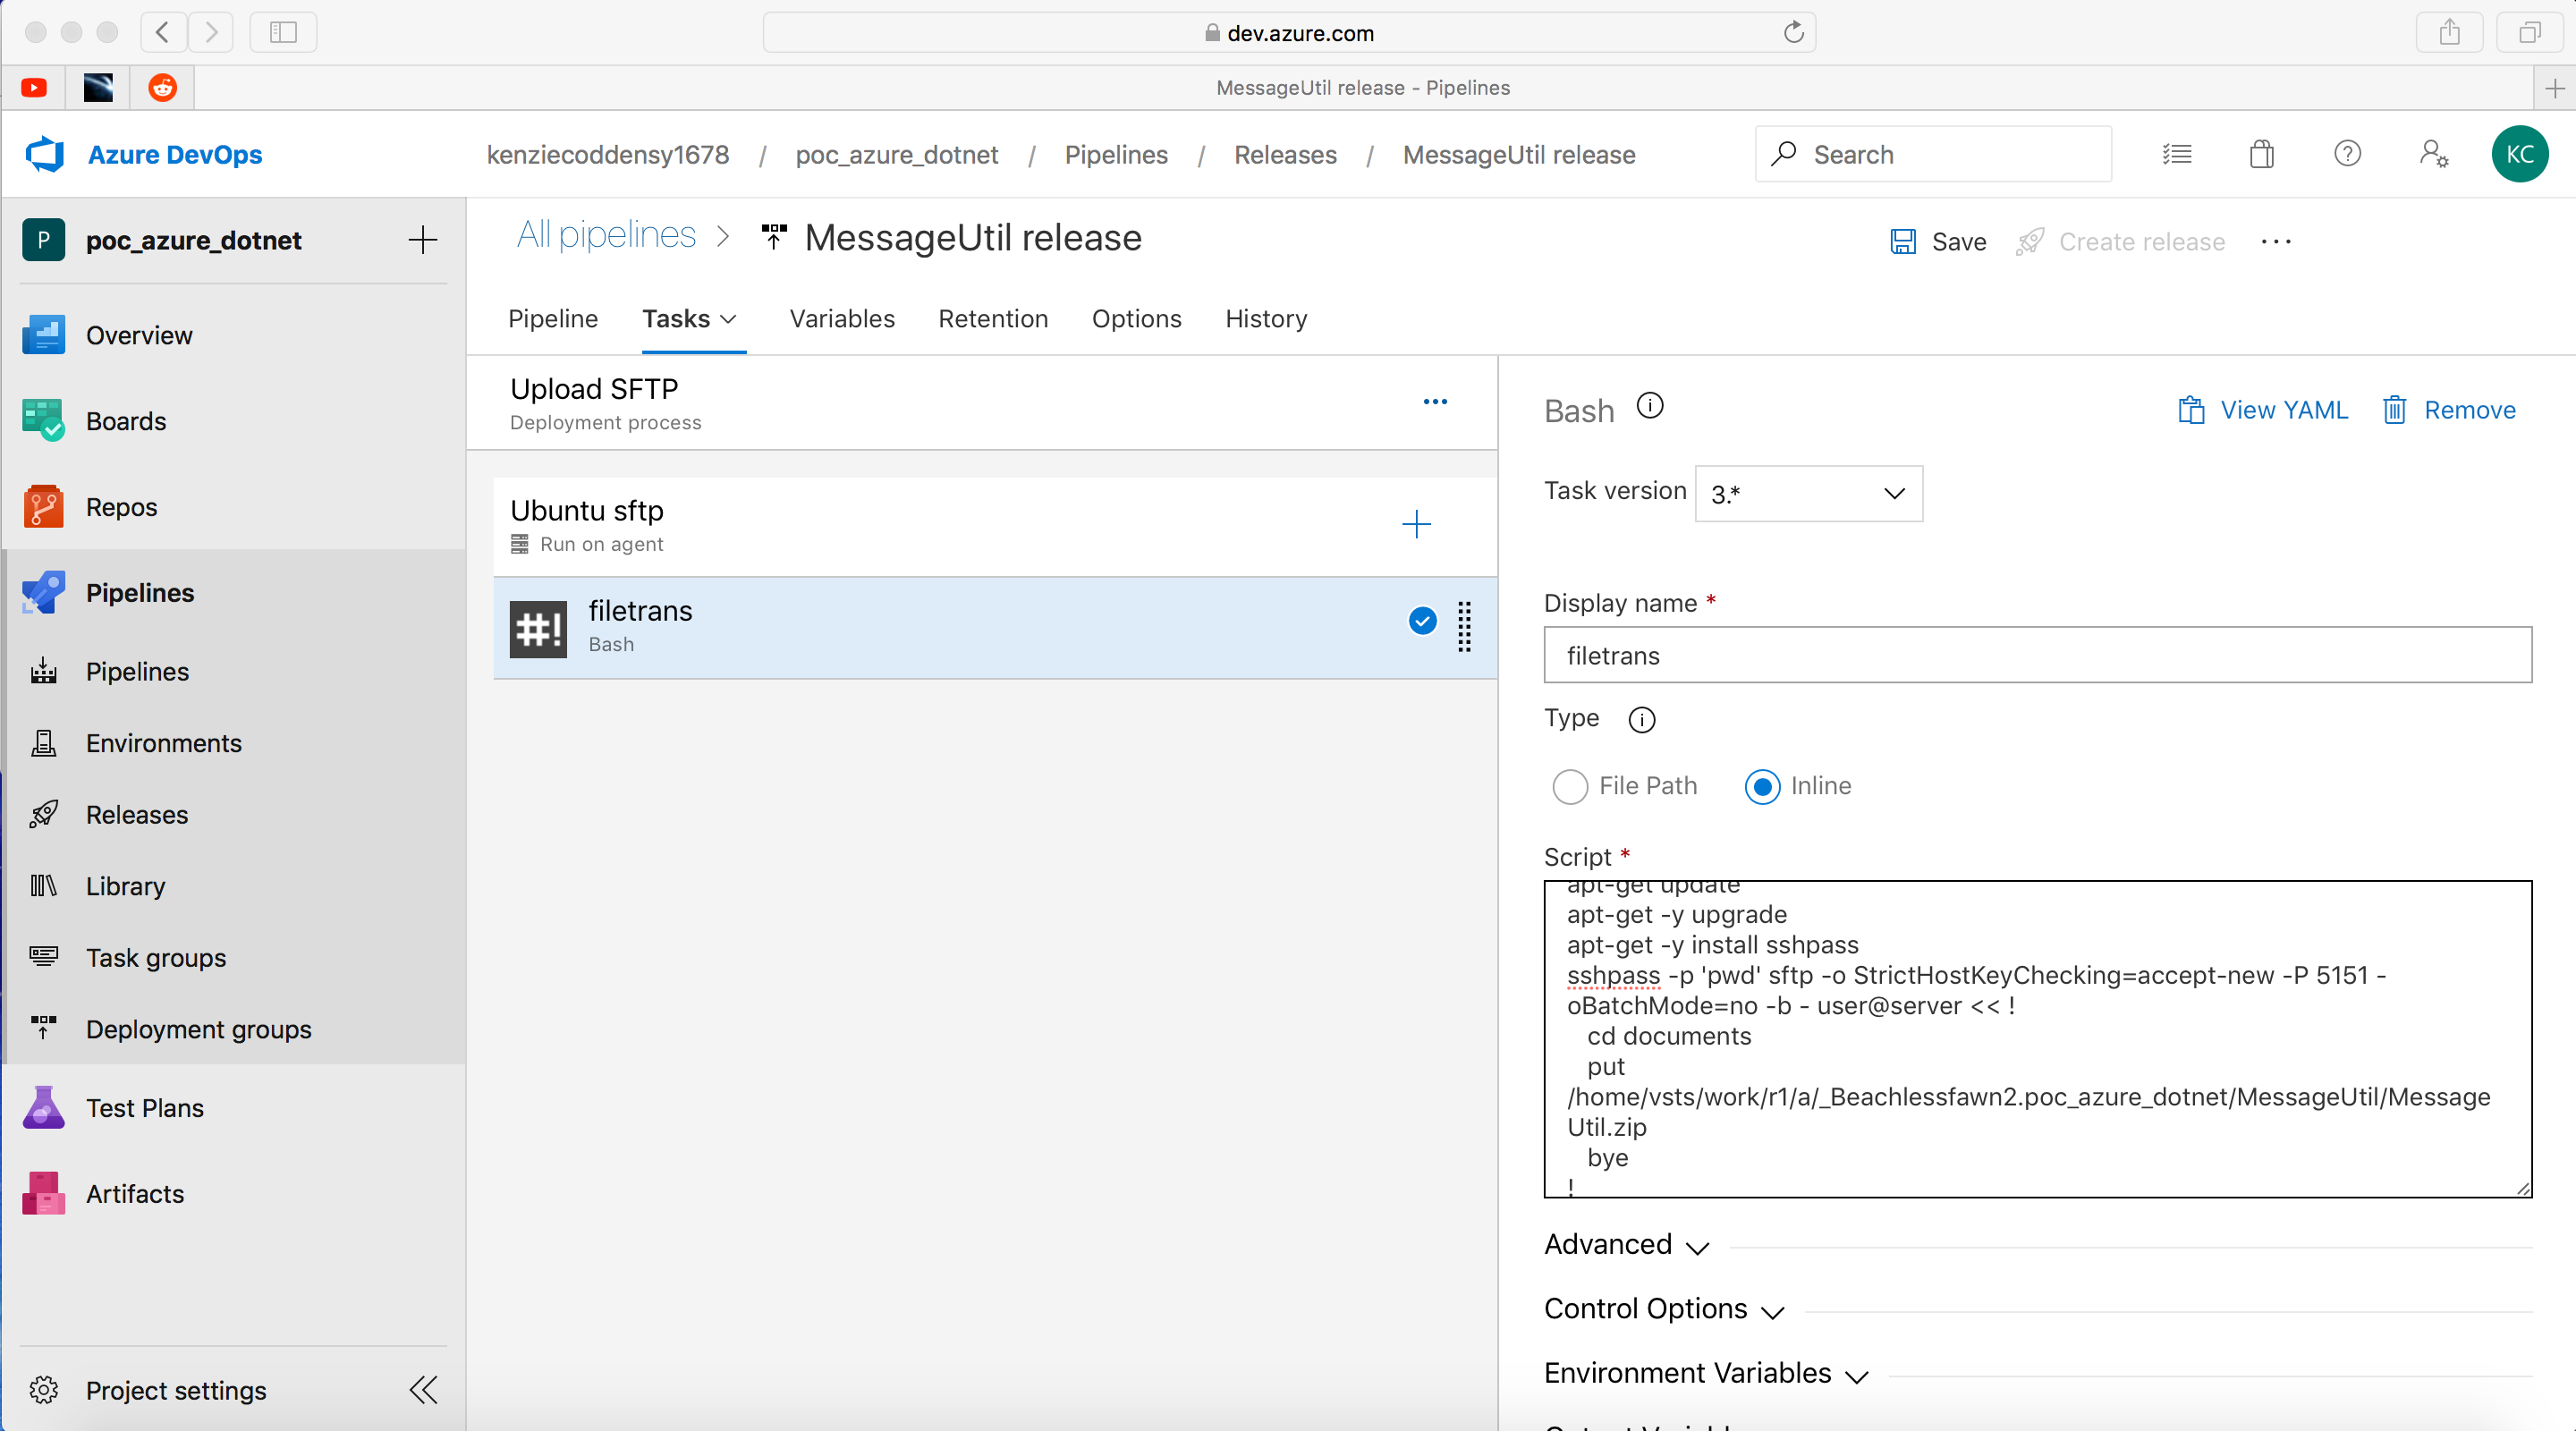
\includegraphics[width=\linewidth]{/Users/kenzie/Documents/HoGent/Bachelorproef/Images/azure_net_demo_release.png}
    \caption{Figuur toont hoe een release pijpleiding op Azure DeVops geconfigureerd wordt. In dit geval wordt er een Ubuntu machine geconfigureerd met een script.}
    \label{fig:Azure_POC_release}
\end{figure}

\begin{figure}[!htbp]
    \centering
    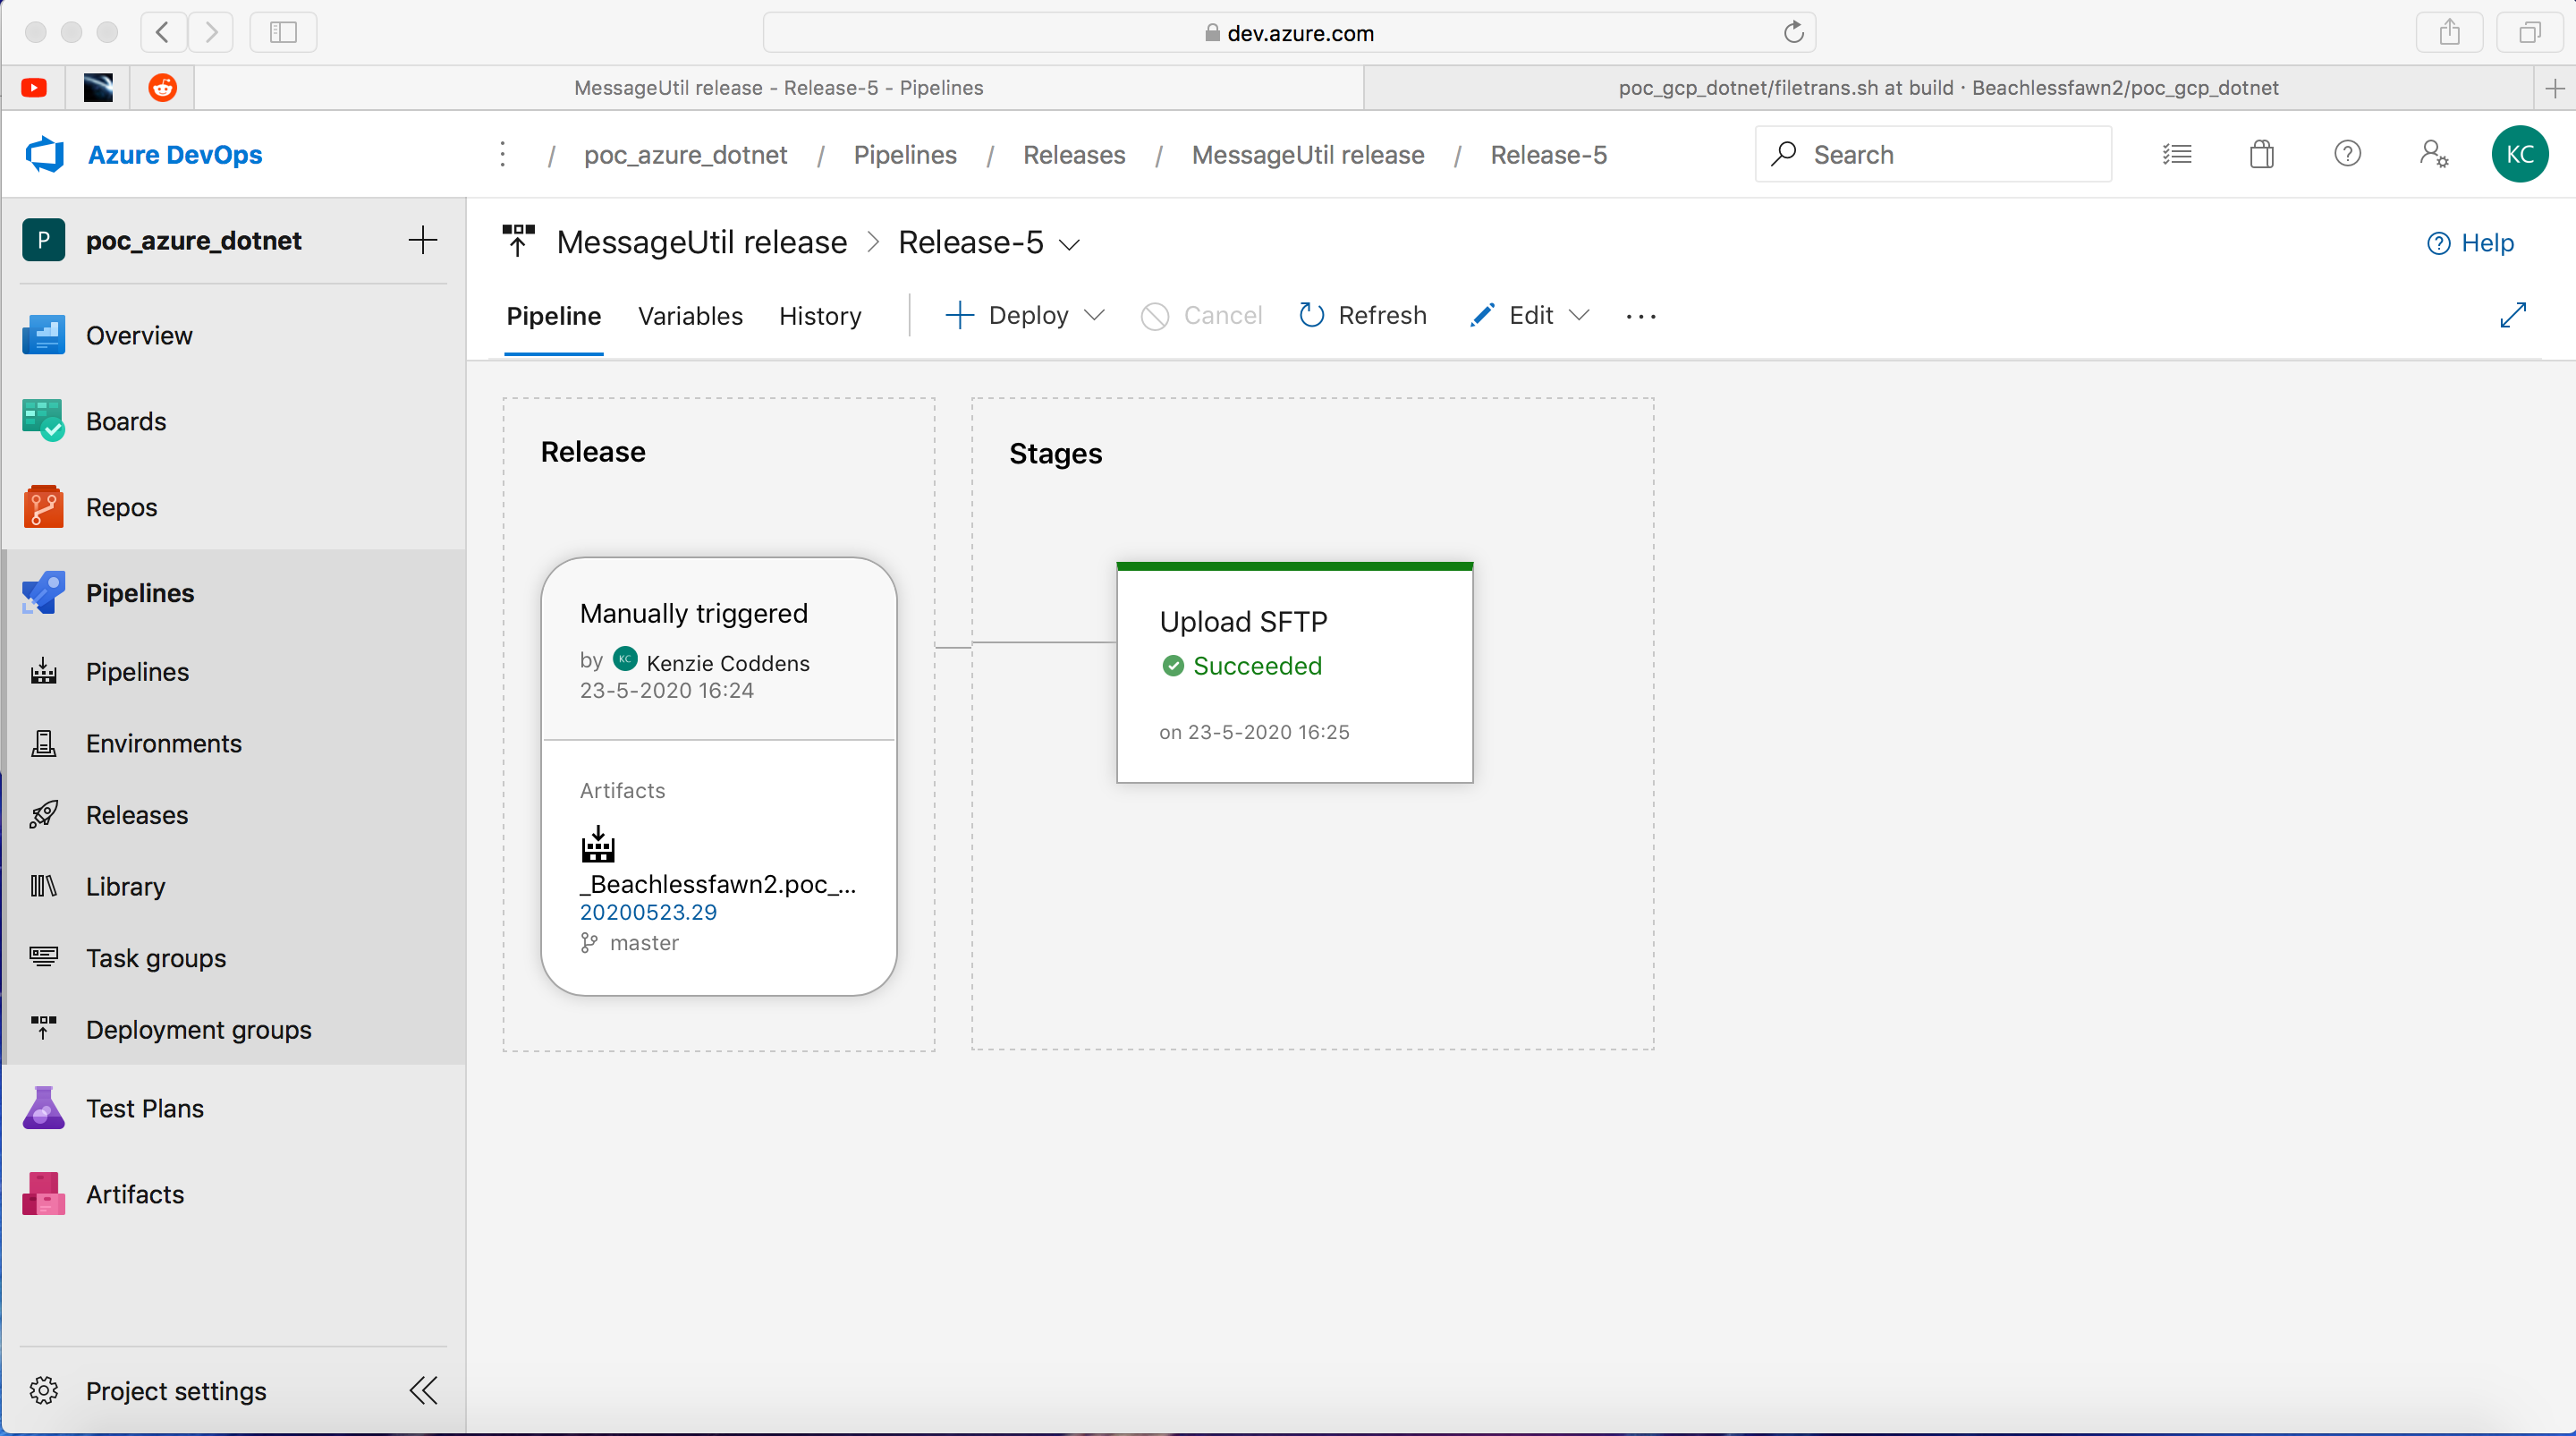
\includegraphics[width=\linewidth]{/Users/kenzie/Documents/HoGent/Bachelorproef/Images/azure_net_demo_pijp.png}
    \caption{De figuur toont een kort overzicht van de totaal gemaakte pijpleiding op Azure DeVops.}
    \label{fig:Azure_POC_pijp}
\end{figure}

Azure DeVops heeft ook zeer goede analytics. Voor deze POC zijn er een aantal voorbeelden gemaakt. Net zoal Google Cloud heeft Azure ook Dashboards. \emph{Figuur~\ref{fig:Azure_POC_dashboard}} toont een overzicht van het project.

\begin{figure}[!htbp]
    \centering
    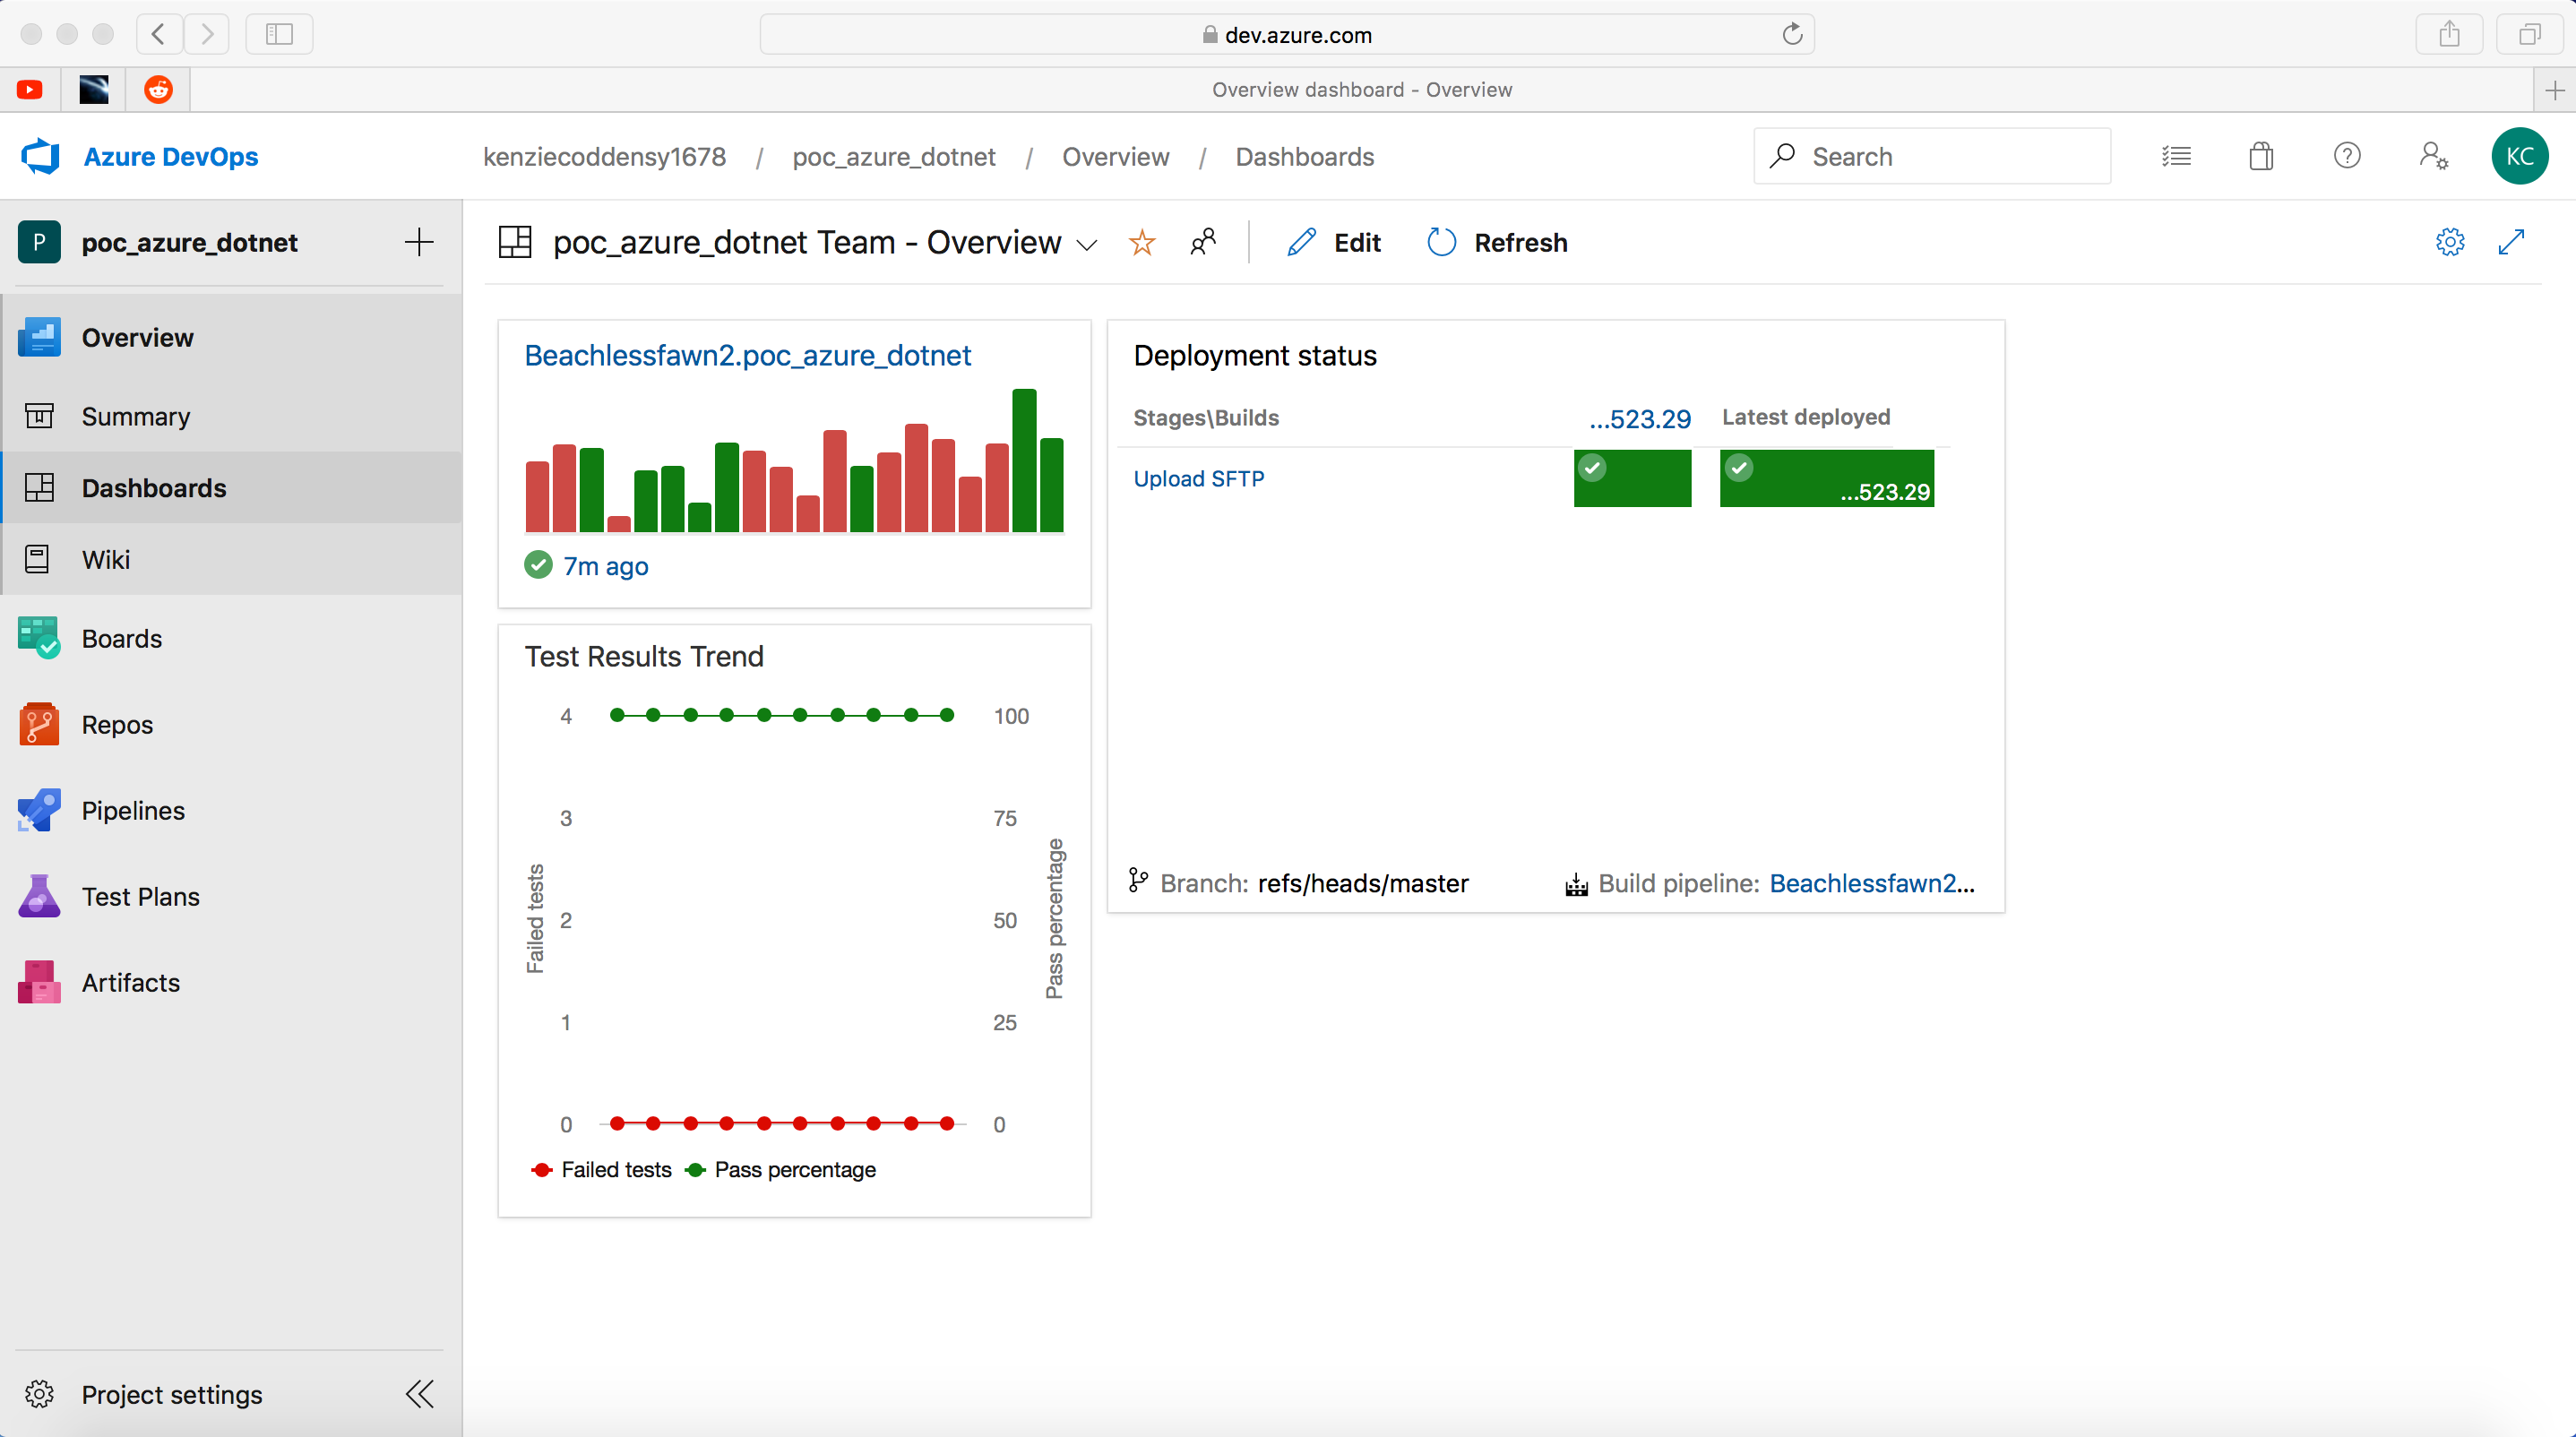
\includegraphics[width=\linewidth]{/Users/kenzie/Documents/HoGent/Bachelorproef/Images/azure_net_demo_dashboard.png}
    \caption{Figuur toont een simpel dashboard met gegevens over de compilatie pijpleiding.}
    \label{fig:Azure_POC_dashboard}
\end{figure}

Uit deze POC is gebleken dat Azure DeVops veel minder complex is om te configureren dan Google Cloud Code Build. Dit komt door de gemakkelijk te gebruiken wizards die de gebruiker door de configuratie heen gidsen. Zo voelt de complexiteit van het configureren van een pijpleiding minder zwaar aan. Uit deze POC is gebleken dat de standaardoplossing die Azure DeVops voorstelt niet altijd even gemakkelijk is om aan te passen naar de gebruiker zijn noden. Deze POC heeft ook aangetoond dat de documentatie van Azure DeVops redelijk complex kan zijn. Zelfs na meerdere projecten te hebben getest, zijn sommige zaken nog niet helemaal duidelijk. Azure DeVops biedt zeer uitgebreide hulpmiddelen aan om allerlei data te visualiseren. Deze dashboards zijn gemakkelijk te creëren. Ook zijn deze zeer duidelijk en overzichtelijk. Dit in tegenstelling tot Google Cloud. In vergelijking met Azure DeVops is Google Cloud gemakkelijker om aangepaste pijpleidingen te maken. Dit omdat het intuïtiever is om de configuratie YAML-bestanden te maken. Ook omdat Google Cloud Code Build met Docker containers werkt. Dit zorgt ervoor dat compileer machines veel uitgebreider kunnen aangepast worden naar de noden van de gebruiker.

Benaderd vanuit het Microsoft ecosysteem is Azure DeVops een zeer goede en logische keuze. Zeker omdat een hele hoop producten en services, die anders aanvullende kosten hebben, vrij te gebruiken zijn. Ook zijn alle hulpmiddelen om software te ontwikkelen volledig geïntegreerd in het platform. Gebruikers die buiten dit ecosysteem werken kijken beter naar Google Cloud in samenwerking met andere tools en oplossingen.


%Aantal woorden: 3933%

% Voeg hier je eigen hoofdstukken toe die de ``corpus'' van je bachelorproef
% vormen. De structuur en titels hangen af van je eigen onderzoek. Je kan bv.
% elke fase in je onderzoek in een apart hoofdstuk bespreken.

%\input{...}
%\input{...}
%...

%%=============================================================================
%% Conclusie
%%=============================================================================

\chapter{Conclusie}
\label{ch:conclusie}

% TODO: Trek een duidelijke conclusie, in de vorm van een antwoord op de
% onderzoeksvra(a)g(en). Wat was jouw bijdrage aan het onderzoeksdomein en
% hoe biedt dit meerwaarde aan het vakgebied/doelgroep? 
% Reflecteer kritisch over het resultaat. In Engelse teksten wordt deze sectie
% ``Discussion'' genoemd. Had je deze uitkomst verwacht? Zijn er zaken die nog
% niet duidelijk zijn?
% Heeft het onderzoek geleid tot nieuwe vragen die uitnodigen tot verder 
%onderzoek?

\lipsum[76-80]



%%=============================================================================
%% Bijlagen
%%=============================================================================

\appendix
\renewcommand{\chaptername}{Appendix}

%%---------- Onderzoeksvoorstel -----------------------------------------------

\chapter{Onderzoeksvoorstel}

Het onderwerp van deze bachelorproef is gebaseerd op een onderzoeksvoorstel dat vooraf werd beoordeeld door de promotor. Dat voorstel is opgenomen in deze bijlage.

% Verwijzing naar het bestand met de inhoud van het onderzoeksvoorstel
%---------- Inleiding ---------------------------------------------------------

\section{Introductie} % The \section*{} command stops section numbering
\label{sec:introductie}
Software release management kan op verschillende manieren geïmplementeerd worden. Dit zijn vaak complexe en zeer use case specifieke omgevingen. Ook testen en debuggen van software en infrastructuur zijn belangrijk voor het afleveren van kwalitatieve producten. Een vraag die hierbij opduikt is of dit op lokale infrastructuur moet gebeuren of op cloud platformen die IaaS (Infrastructure as a Service), TaaS (Testing as a Service) of SaaS (Software as a Service) aanbieden.
\newline
\newline
Der bestaan al tientallen papers over de performantie, flexibiliteit, enz. in een cloud omgeving. Ook over software release management zijn er al talloze papers geschreven. Des ondanks is het toch nog interessant om dit voor een specifieke use case te bekijken. Aucxis heeft al een software release omgeving op Azure. Ze hebben echter geen onderzoek gedaan naar andere cloud platformen of oplossingen. Deze paper is in de eerste plaats bedoelt om voor Aucxis een duidelijk beeld te scheppen over de mogelijkheden.
\newline
\newline
Deze paper zal proberen in detail duidelijkheid te scheppen over wanneer een cloud platform een goede keuze is en wanneer niet, wat de beste tools zijn, hoe het zit met de gebruiksvriendelijkheid en de prijs. Ook de performantie is niet onbelangrijk. Deze paper zal zich ook afvragen hoe data privacy kan gecontroleerd en geïmplementeerd worden. Op het einde van deze paper zal er een conclusie gemaakt worden over welke optie het best past binnen de use case van Aucxis.

%---------- Stand van zaken ---------------------------------------------------

\section{Literatuurstudie}
\label{sec:Literatuurstudie}
\subsection{Conventional Software Testing Vs. Cloud Testing}
Dit artikel \autocite{CSTVCT} snijdt oppervlakkig aan wat pijnpunten kunnen zijn voor testen van software in een cloud platform. Hier gebruiken ze een web applicatie als voorbeeld. Het artikel stelt een aantal punten voor, waarop getest kan worden. Dit zijn de traditionele test cases. Functionaliteit testen, gebruiksvriendelijkheid testen, interface testen, compatibiliteitstesten, performantie testen en tot slot veiligheid en privacy testen. Het artikel stelt een aantal uitdagingen voor bij lokale omgevingen. Dit gaat over de kost, over het onderhoud ervan, hoe eenzijdig een lokale omgeving is en voor ieder project een nieuwe omgeving gebouwd moet worden en het feit dat het geen accurate weergave is van de werkelijke omgevingen waarin de software zal draaien.
\newline
\newline
Verder legt het artikel kort uit wat voor mogelijke cloud oplossingen er op dat moment zijn. Eerst moet er onderscheid gemaakt worden in hoe een cloud platform uitgerold kan worden. Er bestaat enerzijds de publieke cloud (Google Cloud Platform, AWS, Azure, DigitalOcean) en anderzijds een privé cloud. De privé cloud is een lokale opstelling die beschikbaar is over het internet naar andere gebruikers. Ook bestaat er iets zoals een hybride cloud. Hierna wordt er dan nog onderscheid gemaakt tussen welke services deze platformen kunnen aanbieden. Dit artikel beschrijft er drie. SaaS (service as a Service), Paas (Platform as a Service), IaaS (Infrastructure as a Service). Het artikel maakt toch een onderscheid van het traditionele testen. Aangezien het in de cloud mogelijk is om de applicatie te testen op load, stress en capaciteit.
\newline
\newline
Tot slot stelt dit artikel belangrijke uitdagingen aan het licht. Zo is de beveiliging van de data die ontvangen, verstuurd of bewaard worden op een cloud platform belangrijk. Ook zijn er over alle platformen heen weinig tot geen standaarden vastgelegd over zowel de performantie van de systemen als de beschikbaarheid op vlak van aanbod. Het zijn juist deze uitdagingen die belangrijk kunnen zijn voor de onderzoeksvragen.

\subsection{Software Testing Based on Cloud Computing}
In dit artikel \autocite{STBOCC}wordt er opnieuw in detail beschreven wat de verschillende platform mogelijkheden zijn zoals IaaS, PaaS, SaaS. Het artikel probeert ook een definitie te geven aan testen op cloud platformen. Tevens geeft het artikel ook een aantal redenen waarom cloud testen een stuk beter zou zijn dan het testen in lokale omgevingen. Deze komen grotendeels overeen met het vorige artikel. In dit artikel wordt er ook besproken dat beveiliging een groot probleem kan zijn. Juist zoals het vorige artikel wordt er gesteld dat het een echte uitdaging is om test datasets in de cloud te gebruiken aangezien deze meestal afkomstig zijn van een klant. Het artikel bespreekt ook een aantal mogelijkheden om met de cloud te verbinden en testomgevingen te configureren. Het artikel bespreekt vooral virtualisatie.
\newline
\newline
Dit artikel bevestigt deels het vorige artikel. Het geeft wat detail en inzicht in cloud testen. Dit artikel sluit aan met de onderzoeksvragen en geeft richting in probleemgebieden.

\subsection{Benchmarking in the Cloud: What It Should, Can, and Cannot Be}
Zomaar willekeurig testen of experimenten uitvoeren is meestal geen goed idee. Er is nood aan een goed gedefinieerde methode om deze testen uniform uit te voeren. Dit artikel \autocite{BITCWISCACB} beschrijft in extreem detail hoe een cloud platform het best getest kan worden. Er wordt beschreven wat de valkuilen zijn bij performantietesten van een cloud platform. Zo wordt het testen van een lokale omgeving vergeleken met het testen van een cloud omgeving. Dit is een hele uitdaging aangezien de hardware van een cloud platform meestal verschilt en niet hetzelfde is. Het artikel beschrijft het testen van een cloud platform aan de hand van een aantal use cases. Het artikel gebruikt hiervoor use cases die schaalbaar zijn en in pieken benaderd worden. Ook beschrijft het artikel dat het belangrijk is om goed te definiëren wat er allemaal getest moet worden over de verschillende platformen heen.
\newline
\newline
Dit artikel biedt een gedetailleerd inzicht in het opstellen van benchmarks voor cloud omgevingen en zal een belangrijke leidraad vormen voor het opstellen van de experimenten.

\subsection{When to Migrate Software Testing to the Cloud?}
Wanneer moet er gedacht worden om naar een cloud omgeving te migreren? Dit artikel \autocite{WTMSTTTC} beschrijft vanaf wanneer het nuttig is om naar de cloud te migreren. Ook beschrijft het artikel kort wat de ervaring was bij een migratie. Dit artikel is interessant omdat het kort een inzicht geeft in wanneer het nuttig en efficiënt is om naar een cloud te migreren. Dit is interessant omdat dit aansluit bij de probleemstelling of een cloud omgeving voor testen nu zoveel beter kan zijn dan een lokale omgeving.

% Voor literatuurverwijzingen zijn er twee belangrijke commando's:
% \autocite{KEY} => (Auteur, jaartal) Gebruik dit als de naam van de auteur
%   geen onderdeel is van de zin.
% \textcite{KEY} => Auteur (jaartal)  Gebruik dit als de auteursnaam wel een
%   functie heeft in de zin (bv. ``Uit onderzoek door Doll & Hill (1954) bleek
%   ...'')

%---------- Methodologie ------------------------------------------------------
\section{Methodologie}
\label{sec:methodologie}
Een groot deel van de onderzoeksvragen zullen beantwoord worden door onderzoekswerk en vergelijkingen. Zo zal deze paper in detail bespreken welke cloud platformen er bestaan en wat de mogelijk plannen (tarieven en voor gedefinieerde configuraties) zijn. De verschillende platformen zullen op een duidelijke manier naast elkaar gelegd worden en vergeleken worden. Ook zal er gekeken worden naar software release tools. Op basis hiervan zal er dan een keuze gemaakt worden welke platformen er in aanmerking komen voor een proof of concept.
\newline
\newline
Ook zal deze paper methodes beschrijven en testen door middel van experimenten wat betreft het behouden van data privacy. Deze paper zal bijvoorbeeld een experiment uitvoeren met een proxy (een tunnel met encryptie naar het datacenter) om de gebruiksvriendelijkheid hiervan te testen.
\newline
\newline
Na het onderzoek zal er een proof of concept opgezet worden met beste alternatief. Er zal getracht worden om de huidige omgeving van Aucxis zo goed mogelijk te benaderen in functionaliteit. De bedoeling is om dezelfde tools te gebruiken om de omgevingen te monitoren (bijvoorbeeld: een Docker image voor dezelfde configuratie en Telegraf en Grafana voor monitoring). Ook zal er getracht worden om dezelfde testen te gebruiken. Dit alles zal over een bepaalde periode draaiende gehouden worden waarna alle resultaten gebundeld zullen worden. Hierbij zitten ook een aantal subjectieve waarnemingen aangezien er ook onderzoek zal gedaan worden naar gebruiksvriendelijkheid. In deze proof of concept zal er een alternatief platform vergeleken worden met het huidige systeem.
\newline
\newline
\newline
\newline

%---------- Verwachte resultaten ----------------------------------------------
\section{Verwachte resultaten}
\label{sec:verwachte_resultaten}
\subsection{Vergelijking van platformen}
Er wordt verwacht dat de huidige cloud omgeving vanuit de use case van Aucxis de beste oplossing is, zeker op vlak van gebruiksvriendelijkheid en efficiëntie. Ondanks dit wordt er verwacht dat de alternatieven een even goede oplossing zullen aanbieden. Deze zullen waarschijnlijk niet de meest gebruiksvriendelijkste of goedkoopste oplossingen zijn. Voor de tools voor software release management wordt er verwacht dat er gelijkaardige alternatieven aan de huidige tools vanuit de use case gevonden worden.

\subsection{Proof of concept}
Er wordt verwacht dat er een werkende alternatieve omgeving opgezet zal worden die de huidige functionaliteit benaderd. Er wordt verwacht dat de performantie van dit platform op zen minst gelijkaardig is aan de huidige use case. Er wordt verwacht dat de gebruiksvriendelijkheid en de kost verbeteren.

\subsection{beveiliging experiment}

Voor dit experiment zijn er gemengde verwachtingen. Vooral op het vlak van tijdrovende configuraties. Er wordt verwacht dat een proxy het meest flexibel is en het meest gebruiksvriendelijk, zeker als het vergeleken wordt met encryptie of andere tools.

%---------- Verwachte conclusies ----------------------------------------------
\section{Verwachte conclusies}
\label{sec:verwachte_conclusies}
\subsection{Vergelijking van platformen}
Het is moeilijk om een conclusie te voorspellen over welk cloud platform het beste uit de vergelijkingen zal komen. Ook is het moeilijk te voorspellen wat de beste tools zullen zijn. Er wordt wel verwacht dat er een degelijk alternatief voor de huidige oplossing gevonden zal worden. 

\subsection{Proof of concept}
De conclusie zal voor dit experiment zeer duidelijk zijn. Deze zal afhangen van de werking van het alternatief. Is het alternatief sneller, gebruiksvriendelijker, enz. dan zal deze conclusie positief zijn. Anders niet.

\subsection{beveiliging experiment}
Om de data privacy te garanderen wordt er verwacht dat een proxy de beste en meest doenlijke oplossing zal zijn. Het valt moeilijk te zeggen of andere tools of methodes beter zullen presteren.


%%---------- Andere bijlagen --------------------------------------------------
% TODO: Voeg hier eventuele andere bijlagen toe
%\input{...}

%%---------- Referentielijst --------------------------------------------------

\printbibliography[heading=bibintoc]

\end{document}
